%%%%%%%%%%%%%%%%%%%%%%%%%%%%%%%%%%%%%%%%%%%%%%%%%%%%%%%%%%%%% 
% XELATEX
% !TEX TS-program = xelatex
%% Based on a TeXnicCenter-Template by Gyorgy SZEIDL.
%%%%%%%%%%%%%%%%%%%%%%%%%%%%%%%%%%%%%%%%%%%%%%%%%%%%%%%%%%%%%



%------------------------------------------------------------
\documentclass[a4paper,10pt]{report}
\usepackage{fontspec}
\usepackage{amsmath}
\usepackage[hang, small, bf, margin=20pt]{caption}%, tableposition=top
\setlength{\abovecaptionskip}{0pt}
\usepackage{geometry}
\geometry{ a4paper, total={170mm,257mm}, left=10mm,right=10mm, top=20mm,}
\usepackage{makecell}%###################33
\usepackage{graphicx}
\usepackage{subfigure}
\setlength{\parskip}{6pt}
\newtheorem{theorem}{Theorem}
\newtheorem{acknowledgement}[theorem]{Acknowledgement}
\newtheorem{definition}[theorem]{Definition}
%-------------------------------------------
\usepackage{hyperref}
\usepackage{multirow}
\hypersetup{
  colorlinks,
  citecolor=blue,
  filecolor=blue,
  linkcolor=blue,
  urlcolor=blue}
\setcounter{secnumdepth}{3}
% -------------------------------------------------------------
\usepackage{titlesec}
\titleformat{\chapter}[display]
{\normalfont\huge\bfseries\centering}{\thechapter}{20pt}{\Huge}
\newcommand{\cchapter}{\chapter}
\titleformat{\cchapter}[display]
{\normalfont\tiny\bfseries\centering}{\thecchapter}{12pt}{\tiny}
% -------------------------------------------------------------
\usepackage[dvipsnames, table]{xcolor}
\usepackage{mathtools}
\DeclarePairedDelimiter{\ceil}{\lceil}{\rceil}
\usepackage{amssymb}
\usepackage{booktabs}  % for \toprule ...
\usepackage{collcell}
\usepackage{pgf}
\usepackage{setspace}
\usepackage{tikz}
\usetikzlibrary{shapes.geometric}
\usetikzlibrary{arrows.meta,arrows}
\usetikzlibrary{calc,intersections}
\usetikzlibrary{matrix}
\usetikzlibrary{positioning}% To get more advances positioning options
\usetikzlibrary{patterns}
\usepackage{polyglossia}
\usepackage{footnote}
\usepackage{pgfplotstable}% loads pgfplots, tikz, graphicx
%%%%%%%%%%%%%%%%%%%%%%%%%%%%%%%%%%%%%%%%%%%%%%%%%%%%%%%%%%%%%%
% make the tables and the figures centered automatically
\makeatletter
\g@addto@macro\@floatboxreset\centering
\makeatother
%%%%%%%%%%%%%%%%%%%%%%%%%%%%%%%%%%%%%%%%%%%%%%%%%%%%%%%%%%%%%%
\colorlet{LightGreen}{green!25}%for figures
\colorlet{DarkGreen}{green!90}%for figures
\colorlet{LightBlue}{blue!40}%for figures
\colorlet{LightPurple}{red!20}%for figures
\colorlet{LightYellow}{yellow!30}%for figures
\colorlet{LightBlue1}{blue!20}%for figures
\colorlet{LightPurple1}{purple!40}%for figures
%%%%%%%%%%%%%%%%%%%%%%%%%%%%%%%%%%%%%%%%%%%%%%%%%%%%%%%%%%%%%%
\usepackage{listings}
%%%%%%%%%%%%%%%%%%%%%%%%%%%%%%%%%%%%%%%%%%%%%%%%%%%%%%%%%%%%%%
\usepackage{bidipoem}
\setmainlanguage{english}
\setotherlanguage{arabic}
\newfontfamily\arabicfont[Script=Arabic, Scale=1.5]{Scheherazade}
%%%%%%%%%%%%%%%%%%%%%%%%%%%%%%%%%%%%%%%%%%%%%%%%%%%%%%%%%%%%%%
\usepackage{listings}
%%%%%%%%%%%%%%%%%%%%%%%%%%%%%%%%%%%%%%%%%%%%%%%%%%%%%%%%%%%%%%
\definecolor{codegreen}{rgb}{0,0.6,0}%for python code
\definecolor{codegray}{rgb}{0.5,0.5,0.5}%for python code
\definecolor{codepurple}{rgb}{0.58,0,0.82}%for python code
\definecolor{backcolour}{rgb}{0.95,0.95,0.92}%for python code
%%%%%%%%%%%%%%%%%%%%%%%%%%%%%%%%%%%%%%%%%%%%%%%%%%%%%%%%%%%%%%
\lstdefinestyle{mystyle}{
    backgroundcolor=\color{backcolour},   
    commentstyle=\color{codegreen},
    keywordstyle=\color{magenta},
    numberstyle=\tiny\color{codegray},
    stringstyle=\color{codepurple},
    basicstyle=\footnotesize,
    breakatwhitespace=false,         
    breaklines=true,                 
    captionpos=b,                    
    keepspaces=true,                 
    numbers=left,                    
    numbersep=5pt,                  
    showspaces=false,                
    showstringspaces=false,
    showtabs=false,                  
    tabsize=2
}
\lstset{style=mystyle}
%%%%%%%%%%%%%%%%%%%%%%%%%%%%%%%%%%%%%%%%%%%%%%%%%%%%%%%%%%%%
%%%%%%%%%%%%%%%%%%%%%%%%%%%%%%%%%%%%%%%%%%%%%%%%%%%%%%%%%%%%
\tikzset{
  Above/.style={
    midway,
    above,
    font=\scriptsize,
    text width=1.5cm,
    align=center,
  },
  Below/.style={
    midway,
    below,
    font=\scriptsize,
    text width=1.5cm,
    align=center
  }
}
\pgfplotsset{compat=1.11,
  /pgfplots/ybar legend/.style={
    /pgfplots/legend image code/.code={
      \draw[##1,/tikz/.cd,bar width=1pt,yshift=0.0cm,bar shift=0pt]
      plot coordinates {(0cm,0.0cm)};},
  },
}

\pgfplotsset{%
  pointModelsFiguresStyle/.style args={#1}{%
    color=#1,
    mark=0,
    only marks,
    mark size=1.5pt,
    point meta=explicit symbolic,
  }
}

\pgfplotsset{%
  pointRug/.style args={#1}{%
    color=#1,
    mark=-,
    only marks,
    mark size=1.5pt,
    point meta=explicit symbolic,
  }
}

\pgfplotsset{%
  pointBiLSTM/.style args={#1}{%
    color=#1,
    mark=o,
    only marks,
    mark size=1.5pt,
    point meta=explicit symbolic,
  }
}

% LSTM
\pgfplotsset{%
  pointLSTM/.style args={#1}{%
    color=#1,
    mark=square,
    only marks,
    mark size=1.5pt,
    point meta=explicit symbolic,
  }
}

\pgfplotsset{%
  pointBiGRU/.style args={#1}{%
    color=#1,
    mark=pentagon,
    only marks,
    mark size=1.5pt,
    point meta=explicit symbolic,
  }
}

\pgfplotsset{%
  pointGRU/.style args={#1}{%
    color=#1,
    mark=diamond,
    only marks,
    mark size=1.5pt,
    point meta=explicit symbolic,
  }
}
\pgfplotsset{
    azetinaplot/.style={
        width=7cm,
        height=7cm,
        axis lines=middle,
        xlabel=$x$,
        ylabel=$y$,
        enlarge y limits,
        clip=false
    }
}
%%%%%%%%%%%%%%%%%%%%%%%%%%%%%%%%%%%%%%%%%%%%%%%%%%%%%%%%%%%%

%%% Local Variables:
%%% mode: latex
%%% TeX-master: "master"
%%% TeX-engine: xetex
%%% End:


\begin{document}



\thispagestyle{empty}
\begin{centering}
\large{\textbf{\\[1cm]{Learning Meters of Arabic Poems with \\ Deep Learning}}}\\[5cm]
\normalsize{}
A Thesis Presented to the Faculty\\
 of\\
 Nile University\\[5cm]
In Partial Fulfillment\\
of the Requirements for the Degree\\
of Master of Science\\[3cm]
By\\
Moustafa Alaa Mohamed\\
March 2019\\
\end{centering}
\normalsize{}



\newpage 
\thispagestyle{empty}
\begin{centering}
\normalsize{}
CERTIFICATION OF APPROVAL\\[3cm]
Learning Meters of Arabic Poems with \\ Deep Learning\\[4cm]
 By\\
Moustafa Alaa Mohamed\\[4cm]
\end{centering}

\hspace{-1.7em}
\rule[0em]{22em}{0.5pt} \hfill \rule[0em]{14em}{0.5pt} \\
\hspace{1em}
Dr. Samhaa El-Beltagy	(Chair)	\hspace{27.7em} Date\\ %	\hspace{36em}
Professor of Electrical and Computer Engineering \\[1cm]
\hspace{1em}
\rule[0em]{22em}{0.5pt} \hfill \rule[0em]{14em}{0.5pt} \\
\hspace{1em}
Dr. Waleed A. Yousef \hspace{32em}  Date\\ %\hspace{40em}
Associate Professor of Computer Science \\[1cm]
\hspace{1em}
\hspace{1em}
\rule[0em]{22em}{0.5pt} \hfill \rule[0em]{14em}{0.5pt} \\
\hspace{1em}
Dr. Mohsen Rashwan \hspace{31.6em}  Date\\ %\hspace{39.5em}
Professor of Electronics and Electrical\\ Communications Engineering\\[1cm]
\hspace{1em}

\normalsize{}
\newpage 
\pagenumbering{roman} 

\renewcommand{\contentsname}{\uppercase{Table of Contents}}


%%% Local Variables:
%%% mode: latex
%%% TeX-master: "../master"
%%% TeX-engine: xetex
%%% End:


\newpage


\addcontentsline{toc}{chapter}{Dedication}
%\cchapter*{\textit{\LARGE{\mdseries{Dedication}}}}

%\textit{\\To all my family members, especially my mum and dad, to my predestined and future life mate to be by gods will, and to all my lovely friends, who supported me and have always stood by my side through all times.}

\newpage
\addcontentsline{toc}{chapter}{Acknowledgment}
\cchapter*{\LARGE{\mdseries{\uppercase{Acknowledgment}}}}

First and foremost, I would like to thank God for giving me the strength, knowledge, ability and opportunity to undertake this research study and to persevere and complete it satisfactorily. Without His blessings, this achievement would not have been possible. 

I would first like to thank my family,especially Mom, whose dream was to see me achieve this degree -God bless her- and Dad, for the continuous support they have given me throughout my studies; I could not have done it without them. Second, I would like to thank my wife Kholoud for all the love, comfort, and encouragement which motivated me to complete this thesis and my master’s studies at Nile University. 

I would like to thank my supervisor, Associate Professor Waleed A. Yousef, for introducing me to the field of machine learning and guiding me patiently throughout my undergraduate studies and MSc. studies. I am grateful for being given the chance to be part of the Informatics group and to collaborate with such brilliant researchers at Nile University.

I thank the members of my committee, Professors Ahmed Hassan, Samhaa El-Beltagy, Mohsen Rashwan, and Associate Professor Nashwa Abdelbaki, for their valuable time and ideas to enhance this research work. 

I thank all my co-authors, without whom this work would not have been possible, especially Taha M. Madbouly and Omar M. Ibrahime for all their hard work and their dedication to complete this work. 

I thank Mohamed Al-Aggan for his valuable insights in my research. Thanks also to Mohamed Abdel Aziz who helped me during our study in NU. I have met many great people during my studies. To name a couple of my professors who greatly affected my career, I would like to thank Dr.Ayman Ezzat and, Dr.Sameh Al-Ansari. I also need to thank two of my friends who helped me a lot and mentor me: Deyaaeldeen Al-Mahallawi and Omar Marzouk.


%I would like to acknowledge and express my heartfelt gratitude to the persons who have made the achievement of my Master of Science degree possible: \\\\
%Dr. Ahmed Samir Fahmy, for his outstanding assistance and guidance, encouragement, and support all the way.\\\\
%Dr. Ahmed El-Antably, Dr. Nermin Fawzy, and Dr. Mustafa Hunter for their great share and effort in this research.\\\\
%All the Nile University Faculty Members and Staff. \\\\
%Most especially to my family for their help and patience.\\\\
%And above all to God, who have made all things possible.


%%% Local Variables:
%%% mode: latex
%%% TeX-master: "../master"
%%% TeX-engine: xetex
%%% End:



\newpage

\addcontentsline{toc}{chapter}{Table of Contents}
\tableofcontents
\newpage

\addcontentsline{toc}{chapter}{List of Figures} 
\renewcommand\listfigurename{\uppercase{List of Figures}}
\listoffigures 
\newpage

\addcontentsline{toc}{chapter}{List of Tables}
\renewcommand\listtablename{\uppercase{List of Tables}}
\listoftables
\newpage
\pagenumbering{arabic}
\addcontentsline{toc}{chapter}{Thesis Outline}
\begin{spacing}{1}\cchapter*{\LARGE{\mdseries{Thesis Outline}}}\end{spacing}
The following chapters are arranged as follows:
\begin{enumerate}
\item Chapter 1: Presents some basic introduction and background knowledge as regards the Arabic Poem and its definitions. Additionally, it contains details about the Arabic language and some features used during our work.
  \item Chapter 2: Background related to Al-Arud, Deep Learning fundamentals and Literature Review for the previous work on this topic.
  \item Chapter 3: Dataset Design and Experiments. It introduces the Dataset Design acquisition and encoding, including the essential pre-processing steps, and the justification for their need. Pre-processing steps are data extraction, data cleansing, data format, data encoding techniques used. In addition, it contains comparisons between the three techniques used. It presents the model’s details and how we chose the model and the architecture and hyper-parameters details, Model Results, and discussion.
\end{enumerate}

\addcontentsline{toc}{chapter}{Abstract}

\begin{spacing}{1}\cchapter*{\LARGE{\mdseries{ABSTRACT}}}\end{spacing}

People can easily determine whether a piece of writing is a poem or prose, but only specialists can determine the class of poem.

In this thesis, we built a model that can classify poetry according to its meters; a forward step towards machine understanding of the Arabic language.

A number of different deep learning models are proposed for poem meter classification. As poetry is sequence data, then recurrent neural networks are suitable for the task. We have trained three variants of them; LSTM, GRU with different architectures and hyper-parameters. Because meters are a sequence of characters, we have encoded the input text at the character-level, so that we preserve the information provided by the letters succession directly fed to the models. Moreover, we introduce a comparative study on the difference between binary and One-hot encoding regarding their effect on the learning curve. We also introduce a new encoding technique called \textit{Two-Hot}, which merges the advantages of both \textit{Binary} and \textit{One-Hot} techniques.


Artificial Intelligence currently works to do the human tasks such as our problem here. Our target in this thesis is to achieve the human accuracy which will make it easy for anyone to recognise the meter for any poem without referring to the language experts or to study the whole field.

In this thesis, we will explain how to use deep learning to classify the Arabic poem. We will also explain in details the feature of Arabic poem and how to deal with this feature. We explain how anyone can work with Arabic text encoding in a dynamic way to encode the text at the character level and deal with Arabic text features such as the \textit{Tashkeel}.

To the best of the author’s knowledge, this research is the first to address classifying poem meters in a machine learning approach, in general, and in RNN featureless based approach, in particular. In addition, the dataset is the first publicly available dataset prepared for the purpose of future computational research.

%\end{abstract}
%qualitative



%%% Local Variables:
%%% mode: latex
%%% TeX-master: "../master"
%%% TeX-engine: xetex
%%% End:

\newpage

\chapter{\uppercase{Introduction}}\label{Ch:Intro}


%\begin{spacing}{1.5}\section*{\LARGE{\mdseries{Thesis Outline}}}

In this chapter, We will give an introduction and basic background knowledge as regards the Arabic language. Also, it will contain details about Arabic Poetry history and the aim of this thesis.

  Arabic is the fifth most widely spoken language~\cite{Ethnologue_2017}. It is written from right to left. Its
alphabet consists of 28 primary letters, and there are 8 more derived letters
from the basic ones, so the total count of Arabic characters is 36 characters.
The writing system is cursive; hence, most letters join to the letter that comes
after them, a few letters remain disjoint.

\section{Arabic Poetry } %%
%% Introduction; the circumstances before alarud
Arabic poetry(\textarabic{الشعر العربى}) is the earliest form of Arabic literature. It dates back to the Sixth century. Poets have written poems without knowing exactly what rules which make a collection of words a poem. People recognize poetry by nature, but only talented ones can write poems. This was the case until \textit{Al-Farahidi} (718 – 786 CE) has analyzed the
Arabic poetry, then he came up with that the succession of consonants and vowels
produce patterns or \textit{meters}, which make the music of poetry.  He has
counted them fifteen meters.  After that, a student of \textit{Al-Farahidi} has
added one more meter to make them sixteen. Arabs call meters \textarabic{بحور}
which means ``\textit{seas}''. The study of Arabic Poetry Meter Classification is named \textbf{Al-Arud (\textarabic{العَروض})}. It takes too much time for anyone to be an expert in this field. 
\section{Deep Learning}

Deep Learning also named Deep Neural Network is part of Machine Learning algorithms. Deep Learning is trying to simulate the human brain into Neural dependency.  Using Deep Learning, we can achieve better learning results from the data. Deep Neural Network needs a huge amount of data to achieve the expected learning curve and results. It also needs a massive amount of computation to build the networks which are based on an artificial neural network. We used the Recurrent Neural Network (RNN) to work on the Arabic Text which shown its ability to achieve outstanding performance over the text problem data. We also used LSTM to solve the long dependency issue in RNN. We will go deep into the Background section (add deep learning section reference).

\section{Thesis Objectives}
In this study, we work on Poetry Meter Classification and utilize the latest technologies check the class of poem. We also worked to achieve near human expert results which make our work is a breakthrough in the field concerning the results compared to the current achieved results. Figure~\ref{Fig:Thesis_Cycle} shows the steps.,
\begin{figure}[!t]
      \begin{tikzpicture}[>=latex']
        \tikzset{block/.style= {draw, rectangle, align=center,minimum width=2cm,minimum height=1cm},
        rblock/.style={draw, shape=rectangle,rounded corners=1.5em,align=center,minimum width=2cm,minimum height=1cm},
        input/.style={ % requires library shapes.geometric
        draw,
        trapezium,
        trapezium left angle=60,
        trapezium right angle=120,
        minimum width=2cm,
        align=center,
        minimum height=1cm
    },
        }
        \node [rblock]  (start) {Start};
        \node [block, right =1cm of start] (crawl) {Data Crawling};
        \node [block, right =1cm of crawl] (clean) {Data Cleansing};
        \node [block, right =1cm of clean] (encode) {Data Encoding};
        \node [block, below right =2cm and -0.5cm of start] (train) {Training};
        \node [block, right =1cm of train] (validate) {Validation \& Testing};
        \node [block, right =1cm of validate] (choose) {select Best Model};
        \node [rblock, right =1cm of choose] (end) {End};
        \node [coordinate, below right =1cm and 1cm of encode] (right) {};  %% Coordinate on right and middle
        \node [coordinate,above left =1cm and 1cm of train] (left) {};  %% Coordinate on left and middle
        \node [coordinate,below  =1cm and 1cm of validate] (loop) {};  %% Coordinate on left and middle

%% paths
        \path[draw,->] (start) edge (crawl)
                    (crawl) edge (clean)
                    (clean) edge (encode)
                    (encode.east) -| (right) -- (left) |- (train)
                    (train) edge (validate)
                    (validate) -- (loop) -| (train)
                    (validate) edge (choose)
                    (choose) edge (end)
                    ;
    \end{tikzpicture}

%%% Local Variables:
%%% mode: latex
%%% TeX-master: t
%%% End:

  \caption{Thesis Working Steps.}
  \label{Fig:Thesis_Cycle}
\end{figure}

\begin{itemize}
\item Crawling the data from the available sources with labeling.
\item Clean and transform the data.
\item Encode the data into a way to be input to the model to work on it. We used many encoding methods and compared each of them.
\item Train the RNN model into the cleaned data.
\item Validate and test the model.
\item Enhance the model.

\end{itemize}





\clearpage


%\begin{figure}
%	
%	

\begin{tikzpicture}[scale=0.9]
\begin{axis}[
    symbolic x coords={Taweel,
   Kamel,
   Baseet,
   Khafeef,
   Wafeer,
   Rigz,
   Raml,
   Motakarib,
   Sar'e,
   Monsafeh,
   Mogtath,
   Madeed,
   Hazg,
   Motadarik,
   Moktadib,
   Modar'e
    },
    xtick=data,
    % the following x label positioning does work here.
    every axis y label/.style= {at={( 0.1, 1.1)}, anchor=north},
    %ylabel style={font=\footnotesize},
    xticklabel style = {font=\footnotesize},
    ylabel={Class size},
    x=0.4cm,
    x tick label style={rotate=60, anchor=east}, 
    % Y ticks configurations
    y tick label style={/pgf/number format/.cd,%
      scaled y ticks = false,
      set thousands separator={,},
      fixed},]
    \addplot[ybar,fill=myBlue] coordinates {
        (Taweel, 416428)
        (Kamel,  370116)
        (Baseet, 244583)
        (Khafeef,     157880)
        (Wafeer,     143148)
        (Rigz,     119286)
        (Raml,     79560)
        (Motakarib,     63613)
        (Sar'e,     59370)
        (Monsafeh,     28768)
        (Mogtath,     18062)
        (Madeed,     7808)
        (Hazg,     7468)
        (Motadarik,     5144)
        (Moktadib,     799 )
        (Modar'e,     288 )
    };
\end{axis}
\end{tikzpicture}

%	
%	\caption{Meter names are on the $x$-axis, size  is on the $y$-axis.}
%	\label{data_size}
%\end{figure}



%%% Local Variables:
%%% mode: latex
%%% TeX-master: "../master"
%%% TeX-engine: xetex
%%% End:

\newpage


\chapter{\uppercase{Background}}\label{ch_Background}

Each Arabic letter represents a consonant, which means that short vowels are not
represented by the 36 characters, for this reason, the need of \textit{diacritics}
rises. \textit{Diacritics} are symbols that comes after a letter to state the
short vowel accompanied by that letter. There are four diacritics \textarabic{◌َ} \textarabic{◌ُ}
\textarabic{◌ِ} \textarabic{◌ْ} which represent the following short vowels
/\textit{a}/, /\textit{u}/, /\textit{i}/ and \textit{no-vowel} respectively,
their names are \textit{fat-ha, dam-ma, kas-ra and sukun} respectively.  The first
three symbols are called \textit{harakat}. Table \ref{tables:diacritics_dal}
shows the 4 diacritics on a letter.



% table: dal with diacritics
\begin{table}[H]
	\centering
	\begin{tabular}{c c c c c c}
		%\hline
		\toprule
		\textbf{\small{Diacritics}}     & \small{\textit{without}} & \small{\textit{fat-ha}} &
		\small{\textit{kas-ra}} & \small{\textit{dam-ma}} & \small{\textit{sukun}}\\
		%\hline
		\midrule
		\textbf{\small{Shape}}   & \textarabic{د} & \textarabic{دَ} & \textarabic{دِ} &
		\textarabic{دُ} & \textarabic{دْ}\\
		%\hline
		\bottomrule
	\end{tabular}
	\caption{Diacritics on the letter  \textarabic{ د }}\label{tables:diacritics_dal}
\end{table}



There are two more sub-diacritics made up of the basic four to represent two
cases:
\begin{definition}\label{def:shadaa_definition}
  \textbf{Shadaa}  \hfill \\
to indicate the letter is doubled. Any letter with
shaddah (\textarabic{ ّ } ) the letter should be duplicated: first letter with a
constant (sukoon) and second letter with a vowel (haraka) \cite{Alnagdawi2013}; Table  \ref{tables:shadda_dal}
shows the dal with shadda and the original letters.
% table: dal with shadda

\begin{table}[H]
	\centering
	\begin{tabular}{c c c}
		%\hline
		\toprule
		\textbf{\small{Diacritics}} & \small{\textit{letter with Shadda }} & \small{\textit{letters without shadaa  }} \\
		%\hline
		\midrule
		\textbf{\small{Shape}}  & \textarabic{دَّ} &  \textarabic{دْدَ}\\
		%\hline
		\bottomrule
	\end{tabular}
	\caption{Shadaa diacritics on the letter  \textarabic{ د }}\label{tables:shadda_dal}
\end{table}

\end{definition}

\begin{definition}\label{def:tanween_definition}
  \textbf{Tanween} \hfill \\
  %%% \ref{defa} and \ref{defb}
  is doubling the short vowel, and can convert
Tanween fathah, Tanween dhammah or Tanween kasrah by
replacing it with the appropriate vowel ( ُ◌ – dhammah, َ◌ –
fathah or ِ◌ –kasrah ) then add the Noon letter with constant to the end of the word \cite{Alnagdawi2013}. Table \ref{tables:Tanween_dal}
shows the difference between the original letter and the letter with Tanween

\begin{table}[H]
	\centering
	\begin{tabular}{c c c}
		%\hline
		\toprule
		\textbf{\small{Diacritics}} & \small{\textit{letter with tanween }} & \small{\textit{letters without tanween}} \\
		%\hline
		\midrule

          \textbf{\small{Tanween Fat-ha}}  & \textarabic{دً} &  \textarabic{دَ+نْ}\\
          \textbf{\small{Tanween Dam-ma}}  & \textarabic{دٌ} &  \textarabic{دُ+نْ}\\
          \textbf{\small{Tanween Kas-ra}}  & \textarabic{دٍ} &  \textarabic{دِ+نْ}\\


		\bottomrule
	\end{tabular}
	\caption{Tanween diacritics on the letter  \textarabic{ د }} \label{tables:Tanween_dal}
\end{table}


\end{definition}

 Arabs pronounce the sound \textit{/n/} accompanied \textit{sukun} at the end the indefinite words, that sound corresponds to this
letter \textarabic{نْ}, it is called \textit{noon-sakinah}, however, it is
just a phone, it is not a part of the indefinite word, if a word comes as a
definite word, no additional sound is added. Since it is not an essential sound,
it is not written as a letter, but it is written as  \textit{tanween}
\textarabic{◌ٌ ◌ً ◌ٍ}.
% adding tanween and its relationship to the previous letter
\textit{Tanween} states the sound \textit{noon-sakinah}, but as you have noticed,
there are 3 \textit{tanween} symbols, this because  \textit{tanween} is added as
a diacritic over the last letter of the indefinite word, one of the 3 harakat\textit{harakat} accompanies the last letter, the last letter's \textit{harakah}
needs to be stated in addition to the sound \textit{noon-sakinah}, so
\textit{tanween} is doubling the last letter's \textit{haraka}, this way the last
letter's \textit{haraka} is preserved in addition to stating the sound
\textit{noon-sakinah}; for example, \textarabic{رَجُلُ + نْ} is written
\textarabic{رَجُلٌ} and  \textarabic{رَجُلِ + نْ} is written \textarabic{رَجُلٍ}.


Those two definition, Definition ~\ref{def:shadaa_definition} and Definition ~\ref{def:tanween_definition}  will help us to reduce the dimension of the letter's feature vector as we will see in \textit{preparing data} section.


Diacritics makes short vowels clearer, but they are not necessary.
Moreover, a phrase without full diacritics or with just some on some letters is
right linguistically, so it is allowed to drop them from the text.

% Diacritics in Unicode
In Unicode, Arabic diacritics are standalone symbols, each of them has its own
unicode. This is in contrast to the Latin diacritics; e.g., in the set
\textit{\{ê, é, è, ë, ē, ĕ, ě\}}, each combination of the letter \textit{e} and a diacritic is represented by one unicode.

\newpage

\section{Arabic Arud Science}
% @@@ add el3elal and zahafat
% @@@ add tent picture
% @@@ add details into every bahr



\begin{definition}\label{def:arud}
  \textbf{Arud} \hfill \\
  In Arabic Arud natively has many meanings (the way, the direction, the light clouds and Mecca and Madinah \footnote{\textit{Mecca and Madinah are two cities in  Saudi Arabia}.}\cite{AlQuaed}. Arud is the science which studies The Arabic Poem meters and the rules which confirm if the Poem is sound meters \& broken meters. If we need to su
\end{definition}
 
The Author of this science is \textit{Al-Farahidi} (718 – 786 CE) has analyzed the
Arabic poetry; then he came up with that the succession of consonants and vowels
produce patterns or \textit{meters}, which make the music of poetry. He was one of the famous people who know The melodies and the musical parts of speech. He has
counted them fifteen meters.  After that, a student of \textit{Al-Farahidi} has
added one more meter to make them sixteen. Arabs call meters \textarabic{بحور}
which means "\textit{seas}" Poets have written poems without knowing exactly what rules which make a collection of words a poem.

The Reasons which makes \textit{Al-Farahidi} put this science is

  \begin{itemize}
  \item Protect the Arabic Poems from the broken meters.
  \item Distinguish between the original Arabic Poem and the non-poem or from the prose.
    \item Make the rules clear and easy for anyone who needs to write a poem.
  \end{itemize}

  Some people said that the one-day Al-Farahidi was walking into the metal-market and he was said some of the poems and for some reasons the knock of the metals matched the musical sound of the poem he was saying then he got an idea to explore the Arud of the poems.

 There are many reason for this science name 
  \begin{itemize}
  \item It named Arud because some people said he put this science in Arud place \textarabic{العَروض} \textit{with fat-ha, not with dam-ma such as the science name \textarabic{العُروض} } between Mecca and Al-Ta'if\cite{AlQuaed}.
  \item Arud in Arabic is noun come from verb \textarabic{يعرض} which means here to be assessed. They said because of Any poem should be assessed by Al-Arud science so, it named Al-Arud \cite{Alkafi1994}.
  \end{itemize}
  
  

  
    \newpage
    \subsection{Al-Farahidi and Pattern Recognition}
    This subsection is our opinion in Al-Farahidi and his method he followed during working on Arabic Poem Classifications.

\begin{enumerate}


\item Al-Farahidi thought there is a pattern for every collection of the poem by chance; however, He scientifically worked into this problem. He started analyzing the poem and add every group with the same tafa'il to the same class.
\item He analyzed the outliers and the particular case from every class and added it to his model.
\item He revised the Bohor and get the cases and generalize his case to be fit into all Poems.
\item His student once he found some Poems which weren't fit into any model to be a model for a new class.

\end{enumerate}
The best essential point which made us admired by Al-Farahidi is his way of research and his passion for getting an indeed succession model. Also, his model is general and followed all the steps currently any Data scientist follows to explore new pattern. Some people state that He died when he was thinking about the problem he hit a wall which made trouble for him. His die story shows that he was thinking in profoundly about this problem. One of the most interest thing I found during this research is how he found this pattern and Al-Farahidi’s way to find a new thing.
%@@@ add about student for sebayeah
%@@@ التأكد من أن القرآن والحديث ليس شعر وﻹن تصادف فهو ليس قصداً والشعر يجب أن يكون وزناً إتفاقاً

    \newpage
    
    \subsection{Feet Representation}
    A meter is an ordered sequence of feet. Feet are the basic
units of meters; there are ten of them.
\begin{definition}\label{def:feet}
  \textbf{Feet} \hfill \\  A Foot consists of
a sequence of \textbf{Sukun} (Consonants) represented as (0) and \textbf{Harakah} (Vowels) (/). Traditionally, feet are represented by mnemonic words called tafa’il \textarabic{تفاعيل}.
\end{definition}

Feets consists of three parts (Reasons \textarabic{أسباب}, Wedge \textarabic{وتد}, Breaks \textarabic{فواصل}).
\begin{itemize}
\item \textbf{Reasons (\textarabic{أسباب})}: It has two types
  \begin{enumerate}
  \item \textbf{Light (\textarabic{سبب خفيف})} which happens when we have the first letter is harakah and the second is sukun (/0) example (\textarabic{هَبْ, لَمْ}).
    \item \textbf{Heavy (\textarabic{سبب ثقيل})} which happens when we have two harakah letter (//) example (\textarabic{لَكَ, بِكَ}).
    \end{enumerate}
    \item \textbf{Wedge (\textarabic{وتد})}: It has two types
  \begin{enumerate}
  \item \textbf{Combined Wedge (\textarabic{وتد مجموع})} which happens when we have two harakah letters followed by sukun (//0) example (\textarabic{مَشَى, عَلَى}).
    \item \textbf{Separated Wedge (\textarabic{وتد مفروق})} which happens when we have two harakah and in between a sukun letter (/0/) example (\textarabic{مُنْذُ, مِصْرُ}).
    \end{enumerate}
    \item \textbf{Breaks (\textarabic{فواصل}}): It has two types
  \begin{enumerate}
  \item \textbf{Small Break (\textarabic{فاصلة صغرى}}) which happens when we have three harakah letters followed by a sukun letter (///0) example (\textarabic{ذَهَبُوا, سُفُناً}).
    \item \textbf{Big Break (\textarabic{فاصلة كبرى}}) which happens when we have four harakah letters followed by a sukun letter  (////0) example (\textarabic{جَعَلَهُمْ}).\footnote{\textit{Some of Arab linguistic scientist assume the small Breaks as a combination between big reason and small reason. Same for the Big Breaks assumed to be a combination between Big reason and Combined Wedge. So, they didn't assume we have three types of feet it is only pure two and any other feets constructed from this two. In this thesis we assume there are three feets }.}
    \end{enumerate}
  \end{itemize}

\newpage
  \subsubsection{Rules for Arabic Letters Representation}
  Arabic Arud has one general rule in the poem representation which is we represent only the letters which is (spoken) not the written which means the letters with phonatics not the written. We have give the below rules as a results of the general rule.

  \begin{itemize}
  \item Any letter with \textit{harakah} represented as (/).
  \item Any letter with \textit{sukun} represented as (0).
  \item Any letter with shaddah represented by two letters the first one will be \textit{sukun} and the second letter will be \textit{harakah} represented as (0/) example (\textarabic{مُحَمََّد}) will be (//0//0).
  \item Any letter with tanween represented by two letters the first one is \textit{haraka} (/) and the second is \textit{sukun}.
  \item Alef without hamze (\textarabic{همزة الوصل}) and Wow Algmaa are not represented example (\textarabic{وُاعلَموا}) will be (/0//0)
  \item If we have a letter which is not written but (spoken) so, we will represent it example (\textarabic{هذا}) it include Alef but not written (\textarabic{هاذا}) the representation will be (/0/0).
  \item If we have \textit{Meem Aljamaa} with harakah so, it represented with \textit{Mad} example (\textarabic{هُمُ}) will be (//0) .
  \item \textit{Alef Mad} (\textarabic{آ}) will be two letters \textit{Alef with harakah} and \textit{Alef with sukun} example (\textarabic{آدَمُ}) will be (/0//).
    \item if the verse ended with \textit{harkah} we will add \textit{sukun} to it.


    \end{itemize}
Example: (note: the below representation first line is simliar the second one but with Arud language style ).
\begin{Arabic}
  \begin{traditionalpoem*}

    أرَاكَ عَصِيَّ الدّمعِ شِيمَتُكَ الصّبرُ، *** أما للهوى نهيٌ عليكَ ولا أمرُ ؟
     أرَاكَ عَصيْيَ دّمعِ شِيمَتُكَ صّبرُو، ***  أما للهوى نهينْ عليكَ ولا أمرو ؟
    
	\end{traditionalpoem*}
\end{Arabic}
%@@@ add example the difference between arud writting and the actual writing
\newpage

\subsection{Arabic Poetry Feets}

Arabic poetry feets has ten tafa'il \textarabic{تفاعيل} (scansion)  any peom constructed from these feets. They are eight from writing (syntax) perspective, But it ten in the rules.
\begin{savenotes}

\begin{table}[H]
  \centering
  \begin{tabular}{|c|c|c|c|}
    \hline
    \textbf{\#} & \textbf{Feet} & \textbf{Scansion} & \textbf{Construction} \\
    \hline
    1 & \textarabic{فَعُولُنْ}  & \texttt{0/0//} & combined wedge (\textarabic{فعو}) and small reason (\textarabic{لن})   \\
    2 &\textarabic{مَفاعِيلُنْ}& \texttt{0/0/0//} & combined wedge (\textarabic{مفا}) and two light reasons (\textarabic{عي}) (\textarabic{لن})   \\
    3 &\textarabic{مُفَاعَلَتُنْ}& \texttt{0///0//}  &    combined wedge (\textarabic{مفا}), heavy reason (\textarabic{عل}) and light reason (\textarabic{تن}) \\
    4 &\textarabic{فَاعِلاَتُنْ} & \texttt{0/0//0/}   & light reason (\textarabic{فا}), combined wedge (\textarabic{علا}) and light reason (\textarabic{تن})   \\
    5 &\textarabic{فَاعِ لاتُنْ} & \texttt{0/0//0/}  &  Separated wedge (\textarabic{فاع}) and two light reason (\textarabic{لا})(\textarabic{تن}) \footnote{\textit{We separated the letters (\textarabic{ع}) and (\textarabic{لا}) in (\textarabic{فاع لاتن}) to show that this part is separated wedge and distinguish between this feet  and (\textarabic{فاع لاتن}) which contains combined wedge  }.}  \\
    6 &\textarabic{فَاعِلُنْ}  & \texttt{0//0/}   & light reason (\textarabic{فا}) and combined wedge (\textarabic{علن})\\
    7 &\textarabic{مُتَفَاعِلُنْ}& \texttt{0//0///}  & heavy reason (\textarabic{مت}), light reason (\textarabic{فا}) and combined wedge (\textarabic{علن})  \\
    8 &\textarabic{مَفْعُولاَت} & \texttt{0//0///}   & two light reason (\textarabic{مف})(\textarabic{عو}) and separated wedge (\textarabic{لات}) \\
    9 &\textarabic{مُسْتَفْعِلُنْ} & \texttt{0//0/0/}  &  two light reason (\textarabic{مس})(\textarabic{تف}) and combination wedge (\textarabic{علن}) \\
    10 &\textarabic{مُسْتَفْعِ لُنْ} & \texttt{0//0/0/}  & light reason (\textarabic{مس}), separated wedge  (\textarabic{تفع}) and light reason  (\textarabic{لن})\footnote{\textit{We separated the letters (\textarabic{ع}) and (\textarabic{ل}) in (\textarabic{مستفع لن}) to show that it ends with a separated wedge and distinguish between this feet  and (\textarabic{مستفعلن}) which contains combined wedge }}\\


    \hline
  \end{tabular}
  \caption{The ten feet of the Arabic meters. }\label{arud:feet}
\end{table}
    \end{savenotes}

%% Every digit (\texttt{/} or \texttt{0}) represents
%%    the corresponding diacritic over a letter in the feet. \texttt{/} corresponds to
%%    a\textit{harakah} ( \textarabic{◌َ}, \textarabic{◌ُ}, or \textarabic{◌ِ}) and \texttt{0}
%%    corresponds to a \textit{sukun} (\textarabic{◌ْ}). Any \textit{mad} (\textarabic{و, ا, ى}) is
%%    equivalent to \texttt{0}, \textit{tanween} is equivalent to \texttt{0/}, and \textit{shaddah} is
%%    equivalent to \texttt{/0}%

    \newpage
\begin{definition}\label{def:meter}
  \textbf{Meter} \hfill \\
  %%%% What is rtythm,feet
  Poetic meters define the basic rhythm of the poem. Each meter is described by a set of ordered feet which can
be represented as ordered sets of consonants and vowels \cite{Almuhareb2015}.

% \textbf{Some conventions and terminologies}:

% What are poems and terminologies?
% What does a poem look like? bayt, shatr, ....
\begin{Arabic}
	\begin{traditionalpoem*}
          ولد الهدى فالكائنات ضياء *** وفم الزمان تبسم وثناء انشاء
          الروح والملأ الملائك حوله *** للدين والدنيا به بشراء

	\end{traditionalpoem*}
\end{Arabic}%



\end{definition}


\begin{definition}\label{def:verse}
  \textbf{Arabic Verse} \hfill \\ refers to "poetry" as contrasted to prose. Where the common unit of a verse is based on meter or rhyme, the common unit of prose is purely grammatical, such as a sentence or paragraph \footnote{\textit{ https://en.wikipedia.org/wiki/Verse\_(poetry)}.}. A verse know as \textit{Bayt} in Arabic \textarabic{بيت}

\end{definition}


\begin{definition}\label{def:shatr}
  \textbf{Shatr} \hfill \\  A verse consists of two halves, each of them is called \textit{shatr} and carries the full meter.  We will use the term \textit{shatr} to refer to a verse's half; whether the right or the left half.
\end{definition}



\begin{definition}\label{def:poem}
  \textbf{Poem} \hfill \\
  is a set of verses has the same meter and rhyme.

\end{definition}


\newpage

\subsection{Arabic Poetry Meters}

\subsubsection{Al-Taweel \textarabic{الطويل}}
\textbf{Why it named Al-Taweel?}
\textit{Al-Taweel is named Al-Taweel for two reasons; first, It is the longest meter between all meters. Second, It starts with Wedge then Reasons and Wedge is longer than Reasons. So, it named Al-Taweel. We need here to note later in the encoding section we will pad all other meters by zeros to make it all the same length. Example if the max Bayt is 82 so, any Bayt less than 82 will be padded by zeros to have the same length.\cite{Alkafi1994}
  }\\

\textbf{tafa'il}

\begin{Arabic}
	\begin{traditionalpoem*}
          فعلون مفاعيلن فعولن مفاعلن *** فعولن مفاعيلن فعولن مفاعيلن


	\end{traditionalpoem*}
      \end{Arabic}

\textbf{Example:}
\begin{Arabic}
	\begin{traditionalpoem*}
    %$> العصر العباسي >> ابن الفارض
          إذا جادَ أقوامٌ بِمالٍ رأيْتَهُمْ  *** يَجودونَ بالأرواحِ مِنْهُم بِلا بُخلِ
          //0/0 //0/0/0 //0/0 //0//0 *** //0/0 //0/0/0 //0/0 //0/0/0
          فعلون مفاعيلن فعولن مفاعلن *** فعولن مفاعيلن فعولن مفاعيلن

	\end{traditionalpoem*}
      \end{Arabic}

% % % 	% % % % % % % % % % % % % % % % % % % % % % % % % % % % % % % % % % % % % % % % % % % %

\subsubsection{Al-Madeed \textarabic{المديد}}
\textbf{Why it named Al-Madeed?}

\textit{Al-Madeed is named because of the reasons \textarabic{الأسباب} is represented in all its seven parts of tafa'il, One in the first part and the other in the second part. So, it named Madeed \textarabic{مديداً}\cite{Alkafi1994}
  }\\

% @@@note to add references

\textbf{tafa'il}

\begin{Arabic}
	\begin{traditionalpoem*}
فاعلاتن فاعلِن فاعلاتن *** فاعلاتن فاعلن فاعلاتن


	\end{traditionalpoem*}
      \end{Arabic}


\textbf{Example:}

\begin{Arabic}
	\begin{traditionalpoem*}
    % % % العصر الجاهلي >> المهلهل بن ربيعة - الزير
    يَا لِبَكْرٍ أَنْشِرُوا لِي كُلَيْباً	يَا لِبَكْرٍ أَيْنَ أَيْنَ الْفِرَارُ
/0//0/0 /0//0 /0//0/0 *** /0//0/0 /0//0 /0//0/0
فاعلاتن فاعلِن فاعلاتن *** فاعلاتن فاعلن فاعلاتن

	\end{traditionalpoem*}
      \end{Arabic}
\newpage



% % % 	% % % % % % % % % % % % % % % % % % % % % % % % % % % % % % % % % % % % % % % % % % % %

%@@@ check bohor name is same for all latex files
\subsubsection{Al-Baseet \textarabic{البسيط}}

\textbf{Why it named Al-Baseet?}
Al-Baseet there is a different idea behind this name
\begin{itemize}
\item The Reasons \textarabic{الأسباب} expanded into it is tafa'il. So, We will find at the beginning of every part two reasons so; it named Al-Baseet.
\item The other reasons which may be the more logic are the harkat  \textarabic{الحركات} expanded in its tafa'il.\cite{Alkafi1994}
  
\end{itemize}



\textbf{tafa'il}

\begin{Arabic}
	\begin{traditionalpoem*}
مستفعلن فعلن مستفعلن فاعلن *** مستفعلن فاعلن مستفعلن فاعلن


	\end{traditionalpoem*}
      \end{Arabic}


\textbf{Example:}

\begin{Arabic}
	\begin{traditionalpoem*}
          % % % العصر الجاهلي >> المهلهل بن ربيعة - الزير

لَيْسَ الجَمَال بأَثْوابٍ تُزَيِّنُنَا    ***	إن الجمال جمال العلم والأدب
/0/0//0 ///0 /0/0//0 ///0   ***  /0/0//0 ///0 /0/0//0 ///0
مستفعلن فعلن مستفعلن فاعلن  *** مستفعلن فاعلن مستفعلن فاعلن
	\end{traditionalpoem*}
      \end{Arabic}

% % % % % % % % % % % % % % % % % % % % % % % % % % % % % % % % % % % % % % % % % % % % % % %
\subsubsection{Al-Wafer \textarabic{الوافر}}
\textbf{Why it named Al-Wafer?}
Al-Wafer there are different ideas behind this name
\begin{itemize}
\item There is much harakat in its parts because there is no tafa'il has part includes harakat more than the word \textarabic{مفاعلتن}.
\item There are many parts to its base.\cite{Alkafi1994}
\end{itemize}

\textbf{tafa'il}

\begin{Arabic}
	\begin{traditionalpoem*}

          مفاعلتن مفاعلتن مفاعلتن *** مفاعلتن مفاعلتن مفاعلتن

	\end{traditionalpoem*}
      \end{Arabic}


\textbf{Example:}

\begin{Arabic}
  \begin{traditionalpoem*}
    %%% الأولى >> العصر الجاهلي >> عمرو بن كلثوم >> أَلاَ هُبِّي بِصَحْنِكِ فَاصْبَحِيْنَا ( معلقة )
    إِذَا بَلَـغَ الفِطَـامَ لَنَا صَبِـيٌّ *** تَخِـرُّ لَهُ الجَبَـابِرُ سَاجِديْنَـا
    //0///0 //0///0 //0/0 ***  //0///0 //0///0 //0/0
    مفاعلتن مفاعلتن فعولن  *** مفاعلتن مفاعلتن فعولن

	\end{traditionalpoem*}
      \end{Arabic}
\newpage

% % % % % % % % % % % % % % % % % % % % % % % % % % % % % % % % % % % % % % % % % % % % % % %

\subsubsection{Al-Kamel \textarabic{الكامل}}
\textbf{Why it named Al-Kamel?}
\textit{Al-Kamel is named because its harakat is fully integrated and it is 30 harakah which is not similar to any other Bahr has this numbers of harakat. However, Al-wafer has much harakat in its parts but not the same number as Al-Kamel. Al-Wafer has the harakat but it not overwritten into its source but Al-Kamel it is written into its source \textarabic{أصله}. So, Al-Kamel in Arabic named due to it is more integrated  \textarabic{أكمل} than Al-Wafer \cite{Alkafi1994}.
}\\

\textbf{tafa'il}

\begin{Arabic}
	\begin{traditionalpoem*}
متفاعلن متفاعلن متفاعلن *** متفاعلن متفاعلن متفاعلن


	\end{traditionalpoem*}
      \end{Arabic}


\textbf{Example:}

\begin{Arabic}
	\begin{traditionalpoem*}
    % % % الأولى >> العصر الجاهلي >> عنترة بن شداد >> هلْ غادرَ الشُّعراءُ منْ متردَّم ( معلقة )
وَلَقَدْ شَفَا نَفْسِي وَأَبْرَأَ سُقْمَهَا *** قِيلُ الفَوَارِسِ وَيكَ عَنْتَرَ أَقْدِمِ
///0//0 /0/0//0 ///0//0 ***  /0/0//0 ///0//0 ///0//0
متفاعلن مستفعلن متفاعلن *** مستفعلن متفاعلن متفاعلن

	\end{traditionalpoem*}
      \end{Arabic}

% % % % % % % % % % % % % % % % % % % % % % % % % % % % % % % % % % % % % % % % % % % % % % %

\subsubsection{Al-Hazaj \textarabic{الهزج}}
\textbf{Why it named Al-Hazaj?}
\textit{Al-Hazaj is named because of the sound reverberation in its parts. Al-Hazaj in Arabic is sound frequency. So, due to the sound reverberation, it named AL-Hazaj. Also, Because every part ends for two reasons so, it made some of sound like a piece of music to be Al-Hazaj \cite{Alkafi1994}.  }\\

\textbf{tafa'il}

\begin{Arabic}
	\begin{traditionalpoem*}
مفاعيلن مفاعيلن *** مفاعيلن مفاعيلن


	\end{traditionalpoem*}
      \end{Arabic}


\textbf{Example:}

\begin{Arabic}
	\begin{traditionalpoem*}
%%%%أدب .. ابن عبد ربه
          أَيَا مَنْ لاَمَ في الحُبِّ *** وَلَمْ يَعْلَمْ جَوى قَلبي
          //0/0/0 //0/0/0 *** //0/0/0 //0/0/0
          مفاعيلن مفاعيلن *** مفاعيلن مفاعيلن




	\end{traditionalpoem*}
      \end{Arabic}


% % % % % % % % % % % % % % % % % % % % % % % % % % % % % % % % % % % % % % % % % % % % % % %

\subsubsection{Al-Rejz \textarabic{الرجز}}
\textbf{Why it named Al-Rejz?}
\textit{Al-Rejz is named Al-Rezj because it constructed from three parts. If there is an animal and someone pull this animal by one leg and the animal walk into three legs in Arabic named Rejz \textarabic{رجزاً}, this is the reason it named Rejz because of it has three parts similar than animal pulled by one leg and walk into three legs. Also, in Arabic, if we have a camel when it stands up has some disturbances due to it sick or has any issue it named Rejz Camel \textarabic{جمل رجز}, and in Arabic disturbance \textarabic{إضطراب} means Rejz for example \cite{Alkafi1994}.}\\


\textbf{tafa'il}

\begin{Arabic}
  \begin{traditionalpoem*}
    مستفعلن مستفعلن مستفعلن *** مستفعلن مستفعلن مستفعل


	\end{traditionalpoem*}
      \end{Arabic}


\textbf{Example:}

\begin{Arabic}
  \begin{traditionalpoem*}
    دار لسلمى إذ سليمى جارة *** قفر ترى آيانها مثل الزّبر
    /0/0//0 /0/0//0 /0/0//0 *** /0/0//0 /0/0//0 /0/0//0
مستفعلن مستفعلن مستفعلن *** مستفعلن مستفعلن مستفعلن



	\end{traditionalpoem*}
      \end{Arabic}
      % % % % % % % % % % % % % % % % % % % % % % % % % % % % % % % % % % % % % % % % % % % % % % %


\subsubsection{Al-Raml \textarabic{الرمل}}
\textbf{Why it named Al-Raml?}
\textit{Al-Raml is named Al-Raml because Al-Raml is a type of the singing which constructed from this Bahr. Another reason is the Wedges is appeared in between the Reasons so; it named Al-Raml due to the diversity between the Reasons and the wedges inside the tafa'il \cite{Alkafi1994}.}\\

\textbf{tafa'il}

\begin{Arabic}
  \begin{traditionalpoem*}

    فاعلاتن فاعلاتن فاعلاتن *** فاعلاتن فاعلاتن فاعلاتن


	\end{traditionalpoem*}
      \end{Arabic}


\textbf{Example:}

\begin{Arabic}
  \begin{traditionalpoem*}

    إنما الدنيا غرور كلها *** مثل لمغ اﻵل في أرض الفقار
    /0//0/0 /0//0/0 /0//0 *** /0//0/0 /0//0/0 /0//0/0
    فاعلاتن فاعلاتن فاعلن *** فاعلاتن فاعلاتن فاعلاتن


	\end{traditionalpoem*}
      \end{Arabic}


      % % % % % % % % % % % % % % % % % % % % % % % % % % % % % % % % % % % % % % % % % % % % % % %


\subsubsection{Al-Sarea \textarabic{السريع}}
\textbf{Why it named Al-Sarea?}
\textit{Al-Sarea is named Al-Sarea in Arabic Al-Sarea means the fastest. It named these because its speed in teste \textarabic{الزوق} or its parts\textarabic{التقطيع}. The other reason because its three parts have 7 reasons and the reasons are faster than the wedges.\cite{Alkafi1994}}\\

\textbf{tafa'il}

\begin{Arabic}
  \begin{traditionalpoem*}

مستفعلن مستفعلن مفعولات *** مستفعلن مستفعلن مفعولات

	\end{traditionalpoem*}
      \end{Arabic}


\textbf{Example:}

\begin{Arabic}
  \begin{traditionalpoem*}


    أزمان سلمى لا يرى مثلها الر *** راؤون في شام ولا عراق
/0/0//0 /0/0//0 /0//0 *** /0/0//0 /0/0//0 /0//00
مستفعلن مستفعلن مفعولات *** مستفعلن مستفعلن مفعولات



	\end{traditionalpoem*}
      \end{Arabic}



      % % % % % % % % % % % % % % % % % % % % % % % % % % % % % % % % % % % % % % % % % % % % % % %


\subsubsection{Al-Monsareh \textarabic{المنسرح}}
\textbf{Why it named Al-Monsareh?}
\textit{to be written later :) :) \cite{Alkafi1994}.}\\

\textbf{tafa'il}

\begin{Arabic}
  \begin{traditionalpoem*}

مستفعلن مفعولات مستفعلن *** مستفعلن مفعولات مستفعلن

	\end{traditionalpoem*}
      \end{Arabic}


\textbf{Example:}

\begin{Arabic}
  \begin{traditionalpoem*}

    إن ابن زيد لا زال مستعملا *** للخير يفشى فى مصره العرفا
    /0/0//0 /0/0/0/ /0/0//0 *** /0/0//0 /0/0/0/ /0///0
    مستفعلن مفعولات مستفعلن *** مستفعلن مفعولات مفتعلن



	\end{traditionalpoem*}
      \end{Arabic}


      \newpage
      % % % % % % % % % % % % % % % % % % % % % % % % % % % % % % % % % % % % % % % % % % % % % % %


\subsubsection{Al-Khafeef \textarabic{الخفيف}}
\textbf{Why it named Al-Khafeef?}
\textit{Al-Khafeef name in Arabic means light. The reason behind the name is its wedge last harkah connected to its reason so, it became light \textarabic{خفت}. The other reason is its light in teste \textarabic{الزوق} or its parts \textarabic{التقطيع} because it has a part with three reasons and the reasons are lighter than wedges\cite{Alkafi1994}. }\\

\textbf{tafa'il}

\begin{Arabic}
  \begin{traditionalpoem*}

    فاعلاتن مستفع لن فاعلاتن *** فاعلاتن مستفع لن فاعلاتن
    %%%%مستفع لن
	\end{traditionalpoem*}
      \end{Arabic}


\textbf{Example:}

\begin{Arabic}
  \begin{traditionalpoem*}


    حل أهلي ما بين دوني فبادو *** لى وحلّت علوية بالسخال
    /0//0/0 /0/0//0  /0//0/0 *** /0//0/0 /0/0//0 /0//0/0
    فاعلاتن مستفع لن فاعلاتن *** فاعلاتن مستفع لن فاعلاتن


	\end{traditionalpoem*}
      \end{Arabic}

            % % % % % % % % % % % % % % % % % % % % % % % % % % % % % % % % % % % % % % % % % % % % % % %


\subsubsection{Al-Modarea \textarabic{المضارع}}
\textbf{Why it named Al-Modarea?}
\textit{Al-Modarea in Arabic means the present. It named by this name because it is the present version of the Al-Hazaj. Also, This Bahr wasn't famous in Arabic Poem and there weren't any popular peams or poetry used this Bahr before \cite{Alkafi1994}. }\\

\textbf{tafa'il}

\begin{Arabic}
  \begin{traditionalpoem*}

مفاعلين فاع لاتن *** مفاعلين فاع لاتن

  \end{traditionalpoem*}
      \end{Arabic}


\textbf{Example:}

\begin{Arabic}
  \begin{traditionalpoem*}


    كأن لم يكن جديراً *** بحفظ الذي أضاعا
    //0/0/  /0//0/0 *** //0/0/  /0//0/0
    مفاعيل  فاع لاتن *** مفاعيل  فاع لاتن


	\end{traditionalpoem*}
      \end{Arabic}
 \newpage
            % % % % % % % % % % % % % % % % % % % % % % % % % % % % % % % % % % % % % % % % % % % % % % %


\subsubsection{Al-Moktadeb \textarabic{المقتضب}}
\textbf{Why it named Al-Moktadeb ?}
\textit{Al-Moktadeb in Arabic means reproduced from another thing \textarabic{الإقتطاع} and because this Bahr word is all appeared into Al-Monsareh in all its words but also there is a difference in the order of the parts. So, it named Al-Moktadeb because it seems to reproduce from Al-Monsareh. We will have another section which will focus on the relation between the Bohor \cite{Alkafi1994}.  % @@@note to add references of the section
}\\


\textbf{tafa'il}

\begin{Arabic}
  \begin{traditionalpoem*}

مفعولات مستفعلن *** مفعولات مستفعلن

  \end{traditionalpoem*}
      \end{Arabic}


\textbf{Example:}

\begin{Arabic}
  \begin{traditionalpoem*}

    حف كأسها الحبب *** فهي فضة ذهب
    /0//0/  /0///0 *** /0//0/  /0///0
    فاعلات  مفتعلن *** فاعلات مفتعلن




	\end{traditionalpoem*}
      \end{Arabic}

      % % % % % % % % % % % % % % % % % % % % % % % % % % % % % % % % % % % % % % % % % % % % % %


      

      \subsubsection{Al-Mojtaz \textarabic{المجتز}}
\textbf{Why it named Al-Mojtaz?}
\textit{Al-Mojtaz in Arabic name is similar meaning for Al-Moktadeb it means reproduced from another thing \textarabic{الإقتطاع أو الإجتزاز} and because these Bahr words are all appeared into Al-khafeef in all its words but also there is a difference in the order of the parts. So, it named Al-Mojtaz because it seems it reproduced from Al-khafeef \textarabic{إجتُزَّ من بحر الخفيف} \cite{Alkafi1994}.}\\


\textbf{tafa'il}

\begin{Arabic}
  \begin{traditionalpoem*}

    مستفع لن فاعلاتن *** مستفع لن فاعلاتن

	\end{traditionalpoem*}
      \end{Arabic}


\textbf{Example:}

\begin{Arabic}
  \begin{traditionalpoem*}


    أنت الذى ولدتك *** أسماء بنت الحباب
    /0/0//0  ///0/ *** /0/0//0  /0//0/0
    مستفع لن  فعِلاتُ *** مستفع لن فاعلاتن


	\end{traditionalpoem*}
      \end{Arabic}

      \newpage
                  % % % % % % % % % % % % % % % % % % % % % % % % % % % % % % % % % % % % % % % % % % % % % % %


\subsubsection{Al-Motaqareb \textarabic{المتقارب}}
\textbf{Why it named Al-Motaqareb?}
\textit{Al-Motaqareb in Arabic means convergent and is named by this name because the wedges are convergent to each other this is because between every two wedges one reason, so the wedges are convergent to each other. Also, another reason is its parts are similar to each other, so it named Al-Motaqareb \cite{Alkafi1994}.
}
\\

\textbf{tafa'il}

\begin{Arabic}
  \begin{traditionalpoem*}
    فعولن فعولن فعولن فعولن *** فعولن فعولن فعولن فعولن


	\end{traditionalpoem*}
      \end{Arabic}

%%%http://www.uobabylon.edu.iq/uobColeges/lecture_view.aspx?fid=19&depid=1&lcid=31904
\textbf{Example:}

\begin{Arabic}
  \begin{traditionalpoem*}

    فأمَّا تَميمٌ، تَميمُ بنُ مُرٍّ *** فألفاهُمُ القَومُ رَوْبَى، نِياما
    //0/0 //0/0 //0/0 //0/0 *** //0/0 //0/0 //0/0 //0/0
    فعولن فعولن فعولن فعولن *** فعولن فعولن فعولن فعولن




	\end{traditionalpoem*}
      \end{Arabic}

                        % % % % % % % % % % % % % % % % % % % % % % % % % % % % % % % % % % % % % % % % % % % % % % %


\subsubsection{Al-Motadarek \textarabic{المتدارك}}
\textbf{Why it named Al-Motadarek?}
There are different ideas behind this name.
\begin{itemize}
  \item Al-Motadarek in Arabic means explored because Al-Farahidi forgets this Bahr and his student Al-Akhfash Al-Awsat has explored it named by this name.
 %%@@@ (215/830)
  \item Al-Motadarek in Arabic also means followed by something \textarabic{يُدرك}, and because this Bahr came after Al-Motaqareb, it names Al-Motadarek \cite{Alkafi1994}.\\
  \end{itemize}

\textbf{tafa'il}

\begin{Arabic}
  \begin{traditionalpoem*}
فَاْعِلُنْ فَاْعِلُنْ فَاْعِلُنْ فَاْعِلُنْ *** فَاْعِلُنْ فَاْعِلُنْ فَاْعِلُنْ فَاْعِلُنْ
	\end{traditionalpoem*}
      \end{Arabic}

      \textbf{Example:}

\begin{Arabic}
 \begin{traditionalpoem*}
    لَمْ يَدَعْ مَنْ مَضَى لِلَّذِيْ قَدْ غَبَرْ *** فَضْلَ عِلْمٍ سَوَى أَخْذِهِ بِالأثَرْ
    /0//0 /0//0 /0//0 /0//0 *** /0//0 /0//0 /0//0 /0//0
    فَاْعِلُنْ فَاْعِلُنْ فَاْعِلُنْ فَاْعِلُنْ *** فَاْعِلُنْ فَاْعِلُنْ فَاْعِلُنْ فَاْعِلُنْ
 \end{traditionalpoem*}
\end{Arabic}
  
  % % % % % % % % % % % % % % % % % % % % % % % % % % % % % % % % % % % % % % % % % % % % % % % 
  % % % % % % % % % % % % % % % % % % % % % % % % % % % % % % % % % % % % % % % % % % % % % % % 
  \newpage
  \subsection{Bohor Relations}
  to be added :) 
  % % % % % % % % % % % % % % % % % % % % % % % % % % % % % % % % % % % % % % % % % % % % % % % 
  % % % % % % % % % % % % % % % % % % % % % % % % % % % % % % % % % % % % % % % % % % % % % % % 
  % % % % % % % % % % % % % % % % % % % % % % % % % % % % % % % % % % % % % % % % % % % % % % % 



%%% Local Variables:
%%% mode: latex
%%% TeX-master: "../master"
%%% End:

%  \newpage
\clearpage
\section{Deep Learning Background}\label{Sec:Deep_Learning_Background}


\textbf{What is Deep Learning?} \textit{ Deep Learning is a new approach to Machine Learning research which focuses on learning and understanding from the data without the need for a human operator to formally specify all the knowledge that the computer needs. This method is built using a hierarchy of concepts which enables the computer to learn complex concepts by building them layer by layer from simpler ones. A graph which shows how this concept is built will permit us to figure out a very deep graph with many layers; for this reason, we call this approach to AI deep learning~\cite{Goodfellow-et-al-2016}}.\\

There were many early trials to utilize the AI in real life problems. For example, IBM's Deep Blue chess-playing system which defeated world champion Garry Kasprov in 1997 (Hsu, 2002).\\ %@@@@MUST add the reference

Another approach to AI used hard-code knowledge about the world in informal language. A computer can understand statements from the formal language automatically using logical inference rules. This is known as the knowledge base approach to artificial intelligence rules. None of these projects has achieved significant success. For Example, Cyc has tried to gather a comprehensive ontology and knowledge base about the basic concepts of how the world works (Lenat and Guha, 1989).%@@@@MUST add the reference
Cyc is an inference engine and a database of statements in a language called Cycl. A staff of human supervisors enters these statements. People struggle to devise formal rules with sufficient complexity to describe the world accurately~\cite{Goodfellow-et-al-2016}.\\

The difficulty faced in the previous system is because the hard-coded knowledge has shown up the AI need to acquire its knowledge from the data itself. This capability is known as machine learning. This approach has introduced some algorithms which solve and tackle the problems from which we can, for example, check if the email is spam or not. Also, it is used for other problems, such as price predictions for housing. An example of these algorithms is \textit{Naive Bayes} and \textit{Logistic regression}.

This simple machine learning approach is working in the data but not with its original format; it requires some different representation to be input to the model. This different representation is named feature engineering. In the of Feature Engineering deciding whether email is spam or not, it can be word frequency, char frequency, class attributes, capital letters frequency, or some other data processing such as removing stop words from the input lemmatization. So, all the previous features provided by a human expert (who knows the problem in detail and analyzes which of its features affect the data) are then added as a feature to the input model.
   

However, for many tasks, it is difficult to identify the features which should be extracted. For example, we need to detect cars in photographs. We know every car has wheels. So, to detect cars, we can check if there is a wheel to be a feature for car detection. However, to detect or to describe wheels in terms of pixel values is a difficult task. The image may not be clear or may be complicated by shadows, the sun glaring off the metal parts of the wheel, the blurring in images may sometimes make it unclear, and so on~\cite{Goodfellow-et-al-2016}. One solution to this problem is to use machine learning itself to discover not only the output of the model but also the features which are the input for the model. This approach is known as representation learning. Learned representation can achieve better results than hard-designed representation. This approach also allows AI systems to rapidly adapt to new tasks or be automatically identified from any new data. Representation learning can automatically discover many features quickly or can take more time in case of complex tasks, but will at least provide an excellent set of features which can be adapted for any complex problem without the need for manual features. In this research, we used the AI to identify the features for our model, enabling this model to achieve breakthrough results, compared with the old method of manual feature machine learning.

If we go back to the image example, we can show that it is not an easy task to extract features to detect the car from an image. So, Deep Learning is trying to solve this problem in feature engineering by introducing representation learning that build complex representations in terms of another simpler layer of representations. Figure~\ref{Fig:Deep_Learning_Image_Person_Example} shows how deep learning represents an image of a person by combining simpler representation, e.g. the edges and contours which led to understanding complex representations. The benefit from allowing the computer to understand the data and building the representation is the ability to build and understand very complex representation and also to utilize and combine features from simpler to deep representations with many ways such as recurrence or sequences.

Modern deep learning provides a compelling framework for learning data problems. This model becomes more complex by the adding more layers and more units within a layer. The Deep Learning model works perfectly on the big dataset which allows the model to learn the data features in a good way.

In the remaining parts in this section we start introducing the main concepts and components used in deep learning, and the basic units of Recurrent Neural networks and LSTM.%
\begin{figure}[!t] 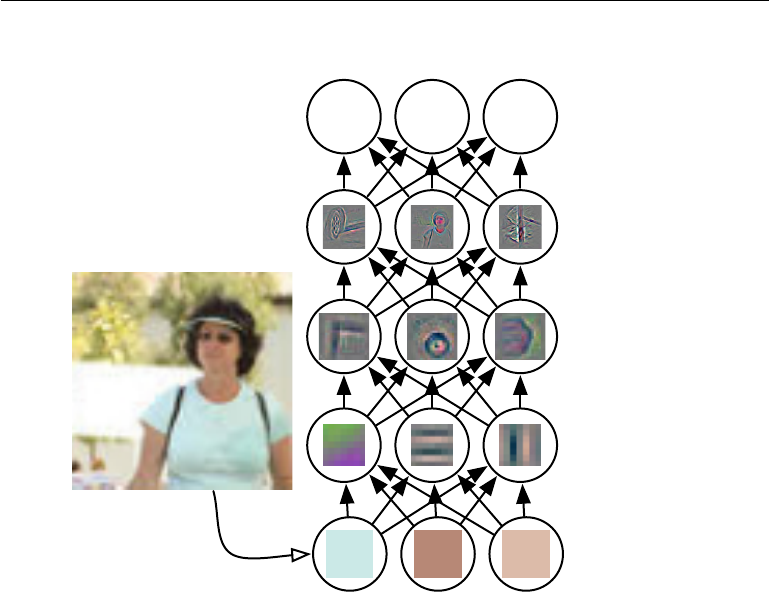
\includegraphics[width=\linewidth]{./Figures/Ch_2_Background/DeepLearningImagePersonExample.png}
 \caption{Illustrations on how Deep Learning can work based on images figure presented~\cite{Goodfellow-et-al-2016}~\cite{Zeiler2014}.}
 \label{Fig:Deep_Learning_Image_Person_Example}
\end{figure}

\subsection{Logistic Regression}


Logistic Regression is a machine learning algorithm which we can assume has the basic idea behind the deep learning (explained later). Logistic Regression is also one of the most used machine learning techniques for binary classification.

A simple example of logistic regression would be an algorithm for fraud detection. It takes some raw data input and detects if it is a fraud case or not. Assume fraud case is one and non-fraud case is zero. David Cox developed logistic regression in 1958~\cite{Cox2958}. The “logistic” name came from its core logistic function, also named \textit{Sigmoid function} function in Equation~\eqref{eq:logistic_function}. The Logistic function is shaped as an S-shape.

One of these function features can take any input real number and convert it into a value between 1 and 0.%
\begin{figure}
\centering
\begin{tikzpicture}
  \begin{axis}%[
%grid=major,
xmin=-10,
xmax=10,
axis x line=bottom,
ytick={0,.5,1},
%xticklabels = {,,}, 
ymax=1,
axis y line=middle,
]
\addplot%
[
blue,%
mark=none,
samples=100,
domain=-10:10,
]
(x,{1/(1+exp(-x))});

%(x,{x^2});
\end{axis}

\end{tikzpicture}%
\caption{Logistic Regression Function (S-Shape)}\label{Fig:Logistic}
\end{figure}%

Example: given x, we want to get the predictions of $\widehat{y}$ which is the estimate of $y$ when $\widehat{y}$ is presented in Equation~\eqref{eq:yhat_estimate}. So, to calculate the output function for Logistic Regression using Equation~\eqref{eq:logistic_regression_yhat}. Note: if we remove the Sigmoid function $\sigma$ from the equation it becomes the Linear Regression model and $\widehat{y}$ can be greater than 1 or negative. Figure~\ref{Fig:Logistic} shows the Sigmoid function output.%
\begin{equation}\label{eq:logistic_function}
 x = \frac{1}{1-e^{-x}} \quad \text{where} \quad x \in \mathbb{R}^{n_x} 
\end{equation}
\begin{equation}
 \label{eq:yhat_estimate}
  \widehat{y} = P(y=1 | x) \quad \text{where} \quad 0 \le \widehat{y} \le 1
 \end{equation}
\begin{equation}
 \label{eq:logistic_regression_yhat}
 \widehat{y} = \sigma(w^t x + b) \quad \text{where:} \quad \sigma(z) = \frac{1}{1-e^{-z}} \text{, } w \in \mathbb{R}^{n_x} \text{, } b \in \mathbb{R} 
\end{equation}%
%
\subsubsection{Loss Error Function}
Loss Error Function is the function which describes how well our algorithm can understand $\widehat{y}$ y b when the true label is y. It also can be defined as the difference between the true value of $y$ and the estimated value of $\widehat{y}$.~\footnote{\textit{Parts of this subsections are explained into Andrew NG Coursera courses in deep learning and written using our understanding of this topic but the equations and the idea is taken from the course}}. Equation~\eqref{eq:loss_function} describe the loss function for Logistic Regression. There are other functions which can represent the loss functions but we take the example below. As we know $y$ is the label which should be 1 or 0, this function makes sense to describe the loss function is outlined below:%
\begin{itemize}
\item in case (y = 1) Equation~\eqref{eq:loss_function} we need $\widehat{y}$ to be as big as possible to be equal or near \textit{y true}, which is 1. So, $ - (\log \widehat{y} )$ will provide the value. Note, as explained before, Sigmoid function can't be greater than 1 or less than 0. 
\item in case (y = 0) Equation~\eqref{eq:loss_function} we need $\widehat{y}$ to be as small as possible to be equal or near \textit{y true}, which is 0. So, $- \log (1-\widehat{y})$ will provide the value. 
\end{itemize}%
%
\begin{equation}
 \label{eq:loss_function}
  \ell(y,\widehat{y}) = - (y \log \widehat{y} + (1-y) \log (1-\widehat{y})) =  \begin{cases}
- (1\times \log \widehat{y} + (1-1) \log (1-\widehat{y})) = - (\log \widehat{y} ) & \mbox{if }  y = 1\\
- (0\times \log \widehat{y} + (1-0) \log (1-\widehat{y})) = - \log (1-\widehat{y}) & \mbox{if } y = 0
\end{cases}
\end{equation}%
%
%\begin{equation} \label{eq:loss_function_log_y_1}
%\begin{split}
% \text{(if y = 1) } \quad \ell(y,\widehat{y}) & = - (y \log \widehat{y} + (1-y) \log (1-\widehat{y})) \\
% & = - (1 \log \widehat{y} + (1-1) \log (1-\widehat{y}))\\
% & = - (\log \widehat{y} )
%\end{split}
%\end{equation}
%\begin{equation} \label{eq:loss_function_log_y_0}
%\begin{split}
% \text{(if y = 0) } \quad \ell(y,\widehat{y}) & = - (y \log \widehat{y} + (1-y) \log (1-\widehat{y})) \\
% & = - (0 \times \log \widehat{y} + (1-0) \log (1-\widehat{y}))\\
% & = - \log (1-\widehat{y})
%\end{split}
%\end{equation}
%
\subsubsection{Cost Function}
To predict $y$ from $\widehat{y}$, we learn from the input parameters in this case it will be \textbf{\textit{(w,b)}} from Equation~\eqref{eq:logistic_regression_yhat} as \textbf{\textit{(w,b)}} are the parameters which define the relation between input dataset X and the output Y. So, Cost Function will measure how well you are doing in an entire training set and the ability to understand the relation between X,Y.

Cost function \textbf{\textit{$J$}} in Equation~\eqref{eq:cost_function} is the average of loss function applied to every training example which equals the sum of the loss for each training example divided by the total number of training examples%
%
\begin{equation}\label{eq:cost_function}
 \begin{split}
 J(w,b) & = \frac{\sum_{i=1}^{m} \ell(y^i,\widehat{y^i})}{m} \quad \text{ where m is the total number of training example} \\
 & = \frac {- \sum_{i=1}^{m} [(y^i \log \widehat{y^i} + (1-y^i) \log (1-\widehat{y^i}))]}{m} 
 \end{split}
\end{equation}%
%
\subsubsection{Convex Function vs Non-Convex Function }

In this subsection we give an overview of the convex and non-convex functions and their relation with deep learning. We do not explain the proofs or write them. We explain in general the definition and its related features to our topic.

\begin{description}
 \item [\textbf{Convex Function}]: In mathematics, a real-valued function defined on an n-dimensional interval is called \textit{convex} if the line segment between any two points on the graph of the function lies above or on the graph, in a Euclidean space (or more generally a vector space) of at least two dimensions~\cite{Wiki_Convex_Function}. More generally, a function $f(x)$ Figure~\ref{Fig:Convex_Function} is \textit{convex} on an interval $[a,b]$ if for any two points $x_1$ and $x_2$ in $[a,b]$ and any $\lambda$ where $0<\lambda<1$~\cite{Rudin_1976},%
%
\begin{equation}\label{eq:convex_fun}
 f(\lambda x_1 + (1-\lambda)x_2) \leq \lambda f(x_1) + (1 - \lambda) f(x_2)
\end{equation}%
%
For a twice differentiable function of a single variable, if the second derivative is always greater than or equal to zero for its entire domain then the function is \textit{convex}. Well-known examples of convex functions include the quadratic function $X^2$ Figure~\ref{Fig:Derivative_Example}. So, If $f(x)$ has a second derivative in $[a,b]$, then a necessary and sufficient condition for it to be \textit{convex} on that interval is that the second derivative $f^{''}(x) \geq 0$ for all $x$ in $[a,b]$~\cite{Wolfram_Convex}.

If the inequality above is strict for all $x_1$ and $x_2$, then $f(x)$ is called \textbf{strictly convex}. \textit{Convex function} on an open set has no more than one minimum. So, in strictly convex, the local minimum = global minimum. This feature is very important for any optimization problem. As we can see, most of deep learning problems are related to how to optimize the function to find the minimum point in this function.  It is an easy problem to face a convex function but in the real world most cases are non-convex functions.

\item [\textbf{Non-Convex Function}]: In mathematics, a Non-Convex (also named concave) function is the negative of a \textit{convex function}. A function $f(x)$ is said to be concave on an interval $[a,b]$ if, for any points $x_1$ and $x_2$ in $[a,b]$, the function $-f(x)$ is convex on that interval.%
\begin{equation}\label{eq:concave_fun}
 \begin{split}
f(\lambda x_1 + (1-\lambda)x_2) \geq \lambda f(x_1) + (1 - \lambda) f(x_2)
 \end{split}
\end{equation}%
The function is also called strictly concave if,
\begin{equation}\label{eq:concave_fun_strictly}
 \begin{split}
f(\lambda x_1 + (1-\lambda)x_2) > \lambda f(x_1) + (1 - \lambda) f(x_2)
 \end{split}
\end{equation}%
%
If $f$ is twice-differentiable, then $f$ is concave if and only if $f^{''}$ is non-positive (or, informally, if the "acceleration" is non-positive). If its second derivative is negative then it is strictly concave, but the opposite is not true, as shown by $f(x) = −x^4$~\cite{Wiki_Concave_Function}. Also, a differentiable function $f$ is (strictly) concave on an interval if and only if its derivative function $f^`$ is (strictly) monotonically decreasing on that interval; that is, a concave function has a non-increasing (decreasing) slope. The problem for non-convex optimization is to find the local minimum. Sometimes many local minimums  can be found and it may be hard to optimize this function Figure~\ref{Fig:Concave_Function}.%
\end{description}
%
\begin{figure}[t]
 \centering
 \subfigure[Convex Function Example]{~\label{Fig:Convex_Function}
 \begin{tikzpicture}[declare function={f(\x)=(\x-1)*(\x-1)/2 +
0.1;},x={(2.5cm,0)},y={(0,2.5cm)},samples=101,font=\small,inner sep=0.5pt]
\draw[-latex] (-0.2,0) -- (3.2,0)  node [right] {$x$};
\draw[-latex] (0,-0.2) -- (0,2.4) node [above] {$y$};
\coordinate (O) at (0,0);
\draw plot[domain=0.2:3,variable=\x] ({\x},{f(\x)});
\foreach [count=\Z] \X/\Y in {0.4/{x_1},2.2/{\lambda x_1 +(1-\lambda) x_2},2.8/{x_2}}
{\draw[dashed] (\X,0) coordinate (X\Z) node[below]{$\strut\Y$} -- (\X,{f(\X)}) coordinate (F\Z)
-- (0,{f(\X)}) node[above right]{$f(\Y)$};}
\draw[blue] (F1) -- (F3);
\draw[dashed] (F2) --
(intersection cs:first line={(X2)--(F2)}, second line={(F1)--(F3)})
coordinate (F4) -- (O|-F4) node[above right]{$f(x_1)+(1-\lambda)\,f(x_2)$};
\foreach \X in {1,...,4}
{\draw[very thin,red,fill=white] (F\X) circle(1pt);}
\end{tikzpicture}}
 \subfigure[Concave Function Example]{~\label{Fig:Concave_Function}
    \begin{tikzpicture}[scale=.7]
     \draw [->] (-1,-0.23) -- (11,-0.23) node [right] {$x$};
     \draw [->] (0,-1) -- (0,8) node [above] {$y$};
     \node at (0,-0.23) [below left] {$0$};
     \draw  plot[smooth, tension=.7] coordinates{(1.5,-0.5) (3,3) (5,1.5)  (7.5,4) (10,-1)};
     \node at (1.75,-0.5) {\scriptsize$a$};
     \node at (9.5,-0.5) {\scriptsize$b$};
     \draw[dashed] (3.2,3.05) -- (3.2,-0.23);
     \draw[dashed] (4.9,1.5) -- (4.9,-0.23);
     \draw[dashed] (7.3,4.05) -- (7.3,-0.23);
     \node at (3.2,-0.5) {\scriptsize$c_{1}$};
     \node at (4.9,-0.5) {\scriptsize$c_{2}$};
     \node at (7.3,-0.5) {\scriptsize$c_{3}$};
     \draw (2.5,3.05) -- (4,3.05);
     \draw (4,1.5) -- (6,1.5);
     \draw (6.5,4.05) -- (8.25,4.05);
     \node at (3.2,3.5) {\scriptsize$f'(c_{1})=0$};
     \node at (4.9,2.2) {\scriptsize$f'(c_{2})=0$};
     \node at (7.3,4.7) {\scriptsize$f'(c_{3})=0$};
     \node at (9.5,3) {\scriptsize$y=f(x)$};
\end{tikzpicture}
}
\caption{Convex and Concave functions examples.}
\end{figure}%
\subsubsection{Gradient Descent}

As we explained previously, we need to find the relation between X,Y from the input parameters \textbf{\textit{(w,b)}} which will make the cost function in Equation~\eqref{eq:cost_function} to the minimum. In other words we need to find the best value of \textbf{\textit{J(w,b)}} which will represent the relation and reduce the error between $y$ and $\widehat{y}$ So, we need to minimize \textbf{\textit{J(w,b)}}.%
%
\begin{figure}[t]
\begin{center}
\begin{figure}[H]
\begin{center}
    \begin{tikzpicture}
    %\draw[step=.5, gray!40, very thin] (0,0) grid (8,4);
\begin{axis}[axis lines=center,
       enlargelimits,
       tick align=inside,
       domain=-1:1,
       samples=30,
       minor tick num=7,]		
       \addplot3 [surf]{x^2+y^2};
       \draw[arrows=-latex,line width=2pt] (2.8cm,-5.2cm) -- (2.8cm,.23cm);
       \draw[thick,fill=purple] (2.8cm,.23cm) circle (0.1cm);
\end{axis}
\end{tikzpicture}
\caption{Gradient Decent }\label{fig:gradient_decent_surf}
\end{center}
\end{figure} 
\caption{Gradient Descent}\label{Fig:gradient_decent_surf}
\end{center}
\end{figure}%
%
To illustrate the relation between \textbf{\textit{J(w,b)}} we assume for simplicity the relation is a function of one variable \textbf{\textit{J(w)}}. As shown in Figure~\ref{Fig:gradient_decent_surf} we have a curve which represents the function \textbf{\textit{J(w)}} we need to find the minimum point in this curve which is the local minimum (red point in the previous figure) assuming it is a \textbf{\textit{convex function}}. we use Equation~\eqref{eq:gredient_descent_w} to find the local minimum.

To explain how this equation works, let's take a simple function $f(x) = x^2$, then select a random point $P_1$ from Figure~\ref{Fig:Derivative_Example}, then pick another point $P_2$. Let's take the derivative \textit{(which by definition is the slope of the function at the point which also the change between these two points)} The slope of this function is the height (3) divided by the width (1); this is the tangent of $J(w)=\frac{3}{1}$ at this point. If the derivative is positive, w will be update minus the derivative multiplied by learning rate alpha $\alpha$ as in Equation~\eqref{eq:gredient_descent_w}. We repeat the previous step until the value of w reaches the minimum. At this point, the derivative is negative, so w will start to increase again; at this step the algorithm will stop. Also, we can demonstrate the effect of different $\alpha$ values and their impact on the function; we can show this effect in Figure~\ref{Fig:Alpha_Change} but the main point is that it is not always a happy scenario. Sometimes the high $alpha$ is not a good idea; it depends on the problem and the dataset.

Now, let's generalize the above equation. Assume we have two parameters \textbf{\textit{(w,b)}} and we need to calculate the cost function for \textbf{\textit{J(w,b)}} we work on as two steps; first function in Equation~\eqref{eq:gradient_descent_j_w} wrt \textbf{\textit{(w)}}, and second function in Equation~\eqref{eq:gradient_descent_j_b} wrt \textbf{\textit{(b)}}%
%
\begin{figure}[!t]
\subfigure[Derivative Example of function $f(x) = x^2$]{~\label{Fig:Derivative_Example}
\begin{figure}[H]
\begin{center}
\begin{tikzpicture}
\draw[step=.5, gray!40, very thin] (0,0) grid (7,5.5);
\begin{axis}[
 % Show (automatically) computed limits:
 title={
  Axis limits are 
  $
 [\pgfmathprintnumber{\pgfkeysvalueof{/pgfplots/xmin}}
 :\pgfmathprintnumber{\pgfkeysvalueof{/pgfplots/xmax}}
 ]  \times 
 [\pgfmathprintnumber{\pgfkeysvalueof{/pgfplots/ymin}}
 :\pgfmathprintnumber{\pgfkeysvalueof{/pgfplots/ymax}}
 ]$ },
]
\addplot {x^2};
% \draw[arrows=-latex,line width=2pt] (2.8cm,-5.2cm) -- (2.8cm,.23cm);
% \draw[arrows=-latex,line width=1pt] (-.07 cm,4.8cm) -- (5.5cm,4cm);


\end{axis}
\draw[line width=1pt] (1,1) -- (4,4);
    \end{tikzpicture}
  
\caption{Derivative Example }\label{fig:derivative_example}
\end{center}
\end{figure} }
\subfigure[Derivative Example of function $f(x) = x^2$ where $\alpha_1$ > $\alpha_2$]{\label{Fig:Alpha_Change}
\begin{tikzpicture}
%\draw[step=.5, gray!40, very thin] (0,0) grid (7,5.5);
\begin{axis}[
% Show (automatically) computed limits:
title={
	Derivative Example with different $\alpha$ values},]
\addplot[mark=*,black,smooth] {x^2};
%\addlegendentry{$f(x)=x^2$};
%\addlegendimage{only marks,mark=*};
%\addlegendimage{only marks,mark=diamond*};
\end{axis}

\draw[arrows=-latex,line width=1pt,blue] (.65,5.2) -- (6,4.5);
\draw[arrows=-latex,line width=1pt,blue] (6,4.5) -- (1.12,3.76);
\draw[arrows=-latex,line width=1pt,blue] (1.12,3.76) -- (5.51,3.15);
\draw[arrows=-latex,line width=1pt,blue] (5.51,3.15)--(1.57,2.6);
\draw[arrows=-latex,line width=1pt,blue] (1.57,2.6)--(5.05,2.1);
\draw[arrows=-latex,line width=1pt,blue] (5.05,2.1)--(2.05,1.7);
\draw[arrows=-latex,line width=1pt,blue] (2.05,1.7) -- (4.55,1.3) ;
\draw[arrows=-latex,line width=1pt,blue]  (4.55,1.3) --(2.55,1);
\draw[arrows=-latex,line width=1pt,blue]  (2.55,1)--(3.88,.65);
\draw[arrows=-latex,line width=1pt,blue]  (3.88,.65)--(3.4,.53);

\draw[arrows=-latex,line width=1pt,red] (.65,5.2) -- (5.51,3.15);
\draw[arrows=-latex,line width=1pt,red] (5.51,3.15)--(2.05,1.7);
\draw[arrows=-latex,line width=1pt,red]  (2.05,1.7) --(3.88,.65);
\draw[arrows=-latex,line width=1pt,red]  (3.88,.65)--(3.4,.53);
\draw[arrows=-latex,line width=1pt,red]  (2.5,-1)-- (3,-1) node [right] {$\alpha_1$};
\draw[arrows=-latex,line width=1pt,blue]  (3.7,-1)-- (4.2,-1) node [right] {$\alpha_2$};
\draw  (2.3, -1.2) rectangle (5, -0.8);


\end{tikzpicture}
}
\end{figure}%
%
\begin{equation}\label{eq:gredient_descent_w}
 \begin{split}
  w & := w - \alpha dw \quad \text{\textit{alpha is learning rate}}\\
   & := w - \alpha \frac{dJ(w)}{dw} \quad \text{\textit{d represent the derivative wrt w}}
 \end{split}
\end{equation}
%
\begin{subequations}
   \begin{align}
w& := w - \alpha \frac{dJ(w,b)}{dw} \label{eq:gradient_descent_j_w}\\
b& := b - \alpha \frac{dJ(w,b)}{db} \label{eq:gradient_descent_j_b}
   \end{align}
 \end{subequations}
%
\subsubsection{Logistic Regression derivatives}\label{Sec:Logistic_Bp_Derivatives}

As described, we need to calculate the gradient descent to get the best $\widehat{y}$ which minimizes the total cost in equation~\eqref{eq:logistic_regression_derivatives_single_example}. So, doing back propagation to get the value of $dz$, we need to calculate $da$ in Equation~\eqref{eq:logistic_regression_derivatives_da}, then calculate $dz$ based on the output of $da$ from Equation~\eqref{eq:logistic_regression_derivatives_dz}. After that, we start to take the derivative for $z$ function parameters \textbf{\textit{$w_1,w_2,b$}}. Once we have the values of \textbf{\textit{$dw_1,dw_2,db$}} we can use them to calculate the estimated values of \textbf{\textit{$w_1,w_2,b$}} in Equations~\eqref{eq:logistic_regression_derivatives_dw1},~\eqref{eq:logistic_regression_derivatives_dw2},~\eqref{eq:logistic_regression_derivatives_db}.%
%
\begin{equation}\label{eq:logistic_regression_derivatives_single_example}
  \boxed{\widehat{y} = \sigma(z) = a} \longrightarrow \boxed{ z = w^tx + b = w_1x_1+ w_2+x_2+ b} \longrightarrow \boxed{\ell(a,y)}
 \end{equation}
 \begin{equation}\label{eq:logistic_regression_derivatives_da}
   \boxed{da = \frac{d\ell}{da} = \frac{d\ell(a,y)}{da} = - \frac{y}{a} + \frac{1-y}{1-a}}
 \end{equation}
  \begin{equation}\label{eq:logistic_regression_derivatives_dz}
  \boxed{dz = \frac{d\ell}{dz} = \frac{d\ell(a,y)}{dz} = \frac{d\ell}{da} . \frac{da}{dz}} = \boxed{(- \frac{y}{a} + \frac{1-y}{1-a}) . a(a-1) } = \boxed{ a - y  }
 \end{equation}
 \begin{equation}\label{eq:logistic_regression_derivatives_dw1}
   \boxed{dw_1 = \frac{\partial\ell}{dw_1} = x_1 dz} \longrightarrow \boxed{ w_1 := w_1 - \alpha dw_1}
 \end{equation}
  \begin{equation}\label{eq:logistic_regression_derivatives_dw2}
  \boxed{dw_2 = \frac{\partial\ell}{dw_2} = x_2 dz} \longrightarrow \boxed{ w_2 := w_2 - \alpha dw_2}
 \end{equation}
 \begin{equation}\label{eq:logistic_regression_derivatives_db}
  \boxed{db = \frac{\partial\ell}{db} = dz} \longrightarrow \boxed{ b := b - \alpha db}
\end{equation}%
%
\subsubsection{Implementing Logistic Regression on m example}
To implement a simple 1 iteration, in the example below the sample code simulates the program structure. First, assume $J = 0, dw_1 = 0, dw_2 = 0,db = 0$. Then calculate the feedforward step. Then backpropagation calculate. Finally, update the parameters. We can transfer the above equation into the below python sample code.%
 \begin{lstlisting}[language=Python]
  import numpy as np
  J = 0, dw_1 = 0, dw_2 = 0,db = 0, alpha = .02
  # FEED FORWARD PROPAGATION
  A = 1 / (1 + np.exp(-(np.dot(w.T,X) + b))#  Z = np.dot(w.T,X) + b
  cost = (- 1 / m) * np.sum(Y * np.log(A) + (1 - Y) * (np.log(1 - A)))
  # BACKWARD PROPAGATION (TO FIND GRADIENT)
  dw = (1 / m) * np.dot(X, (A - Y).T) #  dz = A - Y
  db = (1 / m) * np.sum(A - Y)
  # UPDATE THE PARAMETERS
  w = w - alpha * dw
  b = b - alpha * db
 \end{lstlisting}%
%
\subsection{The Neuron}

Most computer research is trying to simulate the human brain as it is the most advanced creation. If we are trying to check how the model understands the new information, we can give a baby two bananas then ask him about them. The baby can remember it with all it new shapes. Similarly, if you inform any human about some information and trying to get a new inference, it will automatically detect this information. So, the new research tries to simulate the human brain model into an Artificial Intelligence model to achieve this performance. In this subsection, we try to give an overview of the relation between the new research era and the human brain.
 
The neuron is the foundation unit of the brain. The size of the brain is about the size of a grain of rice. The brain contains over 10000 neurons with average 6000 connections with other neurons~\cite{Restak_2001}.  These massive networks allow our brain to build its knowledge about the world around us. The neuron works by receiving the information from other neurons and processes it uniquely then passes the output to other neurons; this process is shown in Figure~\ref{Fig:Neuron_Structure}.%

\begin{figure}[!t] 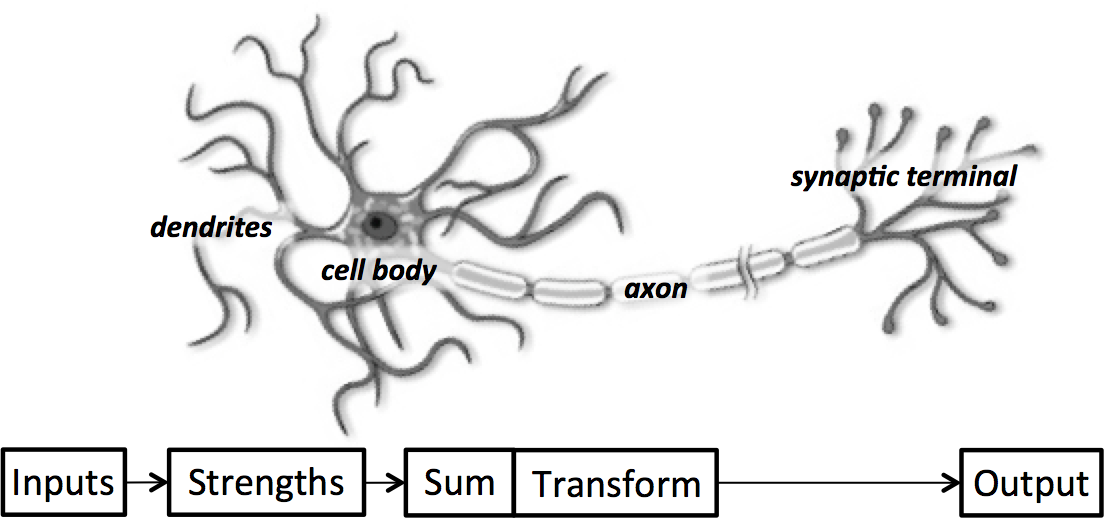
\includegraphics[width=\linewidth]{./Figures/Ch_2_Background/neuron_structure.png}
\caption{Description of neuron's structure this figure from~\cite{DLFundamentals}}
~\label{Fig:Neuron_Structure}
\end{figure}%
 
How do we learn a new concept? \textit{The neuron receives its input from dendrites. The incoming neuron connection is dynamically strengthened or weakened based on how often it is used, and the strength of each connection determines the contribution of the input to the neuron's output. Based on the connection strength, it has weight then the input is summed in the cell body. This sum is transformed into a new signal which is propagated along the cell's axon and sent to other neurons~\cite{DLFundamentals}}.

The above biological model can be translated into an Artificial Neural Network as described in figure~\ref{Fig:NNExample}. We have an input $x_1,x_2,x_3,...,x_n$; every input has its own strength (weight) $w_1,w_2,w_3,...,w_n$. We sum the multiplication of X and W to get the logit of the neuron, $z =  \sum_{i=0}^{n} x_i w_i $. The logit is passed through a function $f$ to produce the output $ y = f(z)$. The output will be the input to other neurons. Note: in many cases, the logit can also include a bias constant. So, in this case the function will be $$ y = f(\sum_{i=0}^{n} x_i w_i + b)$$.
 
\subsection{The Neural Network Representation}
As explained previously, we have been trying to simulate the human brain model into our research work in Deep Neural Network. So, we have multi-layers to allow the model to get in-depth knowledge and more computational performance to simulate the human brain. 

Now, we represent the functions per layer as per the equations below where lt refers to layer number, i refers to the node number in the layer~\eqref{eq:nn_multi_layer}%
%
\begin{equation}\label{eq:nn_multi_layer}
\boxed{z^l = W^l x + b^l} \longrightarrow \boxed{a_i^l = \sigma(z^l)} \longrightarrow \boxed{\ell(a^l,y)}
\end{equation}%
%
What is the Neural Networks component?
Figure~\ref{Fig:NNExample} represents an Example of Neural Networks representations. It consists of

\begin{itemize}
\item \textbf{Input Layer:} Input layer is the input data raw for the network, denoted as $a^0$.
\item \textbf{Hidden Layers:} The layers between the input layers and the output layer can be any number of layers.These have a set of weighted input and produce an output through an activation function. Every layer in the hidden layer transmits the output to the other hidden layer as an input feature.
\item \textbf{Output Layer:} This is one output layer with the final results from the hidden layers.
\end{itemize}

\subsection{Neural Network Computation}

In this subsection, we show as example on how we can compute the Neural Networks for every layer. In figure~\ref{Fig:NNExample} we have an example of Input layer of N input, one hidden layer, and one output layer. We continue explain on this example in Equation~\eqref{eq_nn_one_layer}.%
\begin{figure}[!t]
\begin{tikzpicture}
\node[draw,circle,minimum size=25pt,inner sep=0pt] (x) at (0,0) {$\Sigma$ $\sigma$};

\node[inputNode] (x0) at (-2, 1.5) {$\tiny +1$};
\node[inputNode] (x1) at (-2, 0.75) {$\tiny x_1$};
\node[inputNode] (x2) at (-2, 0) {$\tiny x_2$};
\node[inputNode] (x3) at (-2, -0.75) {$\tiny x_3$};
\node[inputNode] (xn) at (-2, -1.75) {$\tiny x_n$};

\draw[stateTransition] (x0) to[out=0,in=120] node [midway, sloped, above] {$w_0$} (x);
\draw[stateTransition] (x1) to[out=0,in=150] node [midway, sloped, above] {$w_1$} (x);
\draw[stateTransition] (x2) to[out=0,in=180] node [midway, sloped, above] {$w_2$} (x);
\draw[stateTransition] (x3) to[out=0,in=210] node [midway, sloped, above] {$w_3$} (x);
\draw[stateTransition] (xn) to[out=0,in=240] node [midway, sloped, above] {$w_n$} (x);
\draw[stateTransition] (x) -- (4,0) node [midway,above] {$\sigma\left(w_0 + \sum\limits_{i=1}^{n}{w_ix_i}\right)$};
\draw[dashed] (0,-0.43) -- (0,0.43);
\node (dots) at (-2, -1.15) {$\vdots$};
\node[inputNode, thick] (i1) at (6, 0.75) {};
\node[inputNode, thick] (i2) at (6, 0) {};
\node[inputNode, thick] (i3) at (6, -0.75) {};

\node[inputNode, thick] (h1) at (8, 1.5) {};
\node[inputNode, thick] (h2) at (8, 0.75) {};
\node[inputNode, thick] (h3) at (8, 0) {};
\node[inputNode, thick] (h4) at (8, -0.75) {};
\node[inputNode, thick] (h5) at (8, -1.5) {};

\node[inputNode, thick] (o1) at (10, 0.75) {};
\node[inputNode, thick] (o2) at (10, -0.75) {};

\draw[stateTransition] (5, 0.75) -- node[above] {$I_1$} (i1);
\draw[stateTransition] (5, 0) -- node[above] {$I_2$} (i2);
\draw[stateTransition] (5, -0.75) -- node[above] {$I_3$} (i3);

\draw[stateTransition] (i1) -- (h1);
\draw[stateTransition] (i1) -- (h2);
\draw[stateTransition] (i1) -- (h3);
\draw[stateTransition] (i1) -- (h4);
\draw[stateTransition] (i1) -- (h5);
\draw[stateTransition] (i2) -- (h1);
\draw[stateTransition] (i2) -- (h2);
\draw[stateTransition] (i2) -- (h3);
\draw[stateTransition] (i2) -- (h4);
\draw[stateTransition] (i2) -- (h5);
\draw[stateTransition] (i3) -- (h1);
\draw[stateTransition] (i3) -- (h2);
\draw[stateTransition] (i3) -- (h3);
\draw[stateTransition] (i3) -- (h4);
\draw[stateTransition] (i3) -- (h5);

\draw[stateTransition] (h1) -- (o1);
\draw[stateTransition] (h1) -- (o2);
\draw[stateTransition] (h2) -- (o1);
\draw[stateTransition] (h2) -- (o2);
\draw[stateTransition] (h3) -- (o1);
\draw[stateTransition] (h3) -- (o2);
\draw[stateTransition] (h4) -- (o1);
\draw[stateTransition] (h4) -- (o2);
\draw[stateTransition] (h5) -- (o1);
\draw[stateTransition] (h5) -- (o2);

\node[above=of i1, align=center] (l1) {Input \\ layer};
\node[right=2.3em of l1, align=center] (l2) {Hidden \\ layer};
\node[right=2.3em of l2, align=center] (l3) {Output \\ layer};

\draw[stateTransition] (o1) -- node[above] {$O_1$} (11, 0.75);
\draw[stateTransition] (o2) -- node[above] {$O_2$} (11, -0.75);

\path[dashed, double, ultra thick, gray] (x.north) edge[bend left=0] (h5.north);
\path[dashed, double, ultra thick, gray] (x.south) edge[bend right=0] (h5.south);
\end{tikzpicture}

\caption{Neural Networks Example Input layer with N input samples, One hidden Layer, and an Output Layer}~\label{Fig:NNExample}
\end{figure}%
\begin{subequations}\label{eq_nn_one_layer}
\begin{align}
Z_1^{[1]} & = w_1^{[1]T} x + b_1^{[1]} , a_1^{[1]} = \sigma(Z_1^{[1]}) \\
Z_2^{[1]} & = w_2^{[1]T} x + b_2^{[1]} , a_2^{[1]} = \sigma(Z_2^{[1]})\\
Z_3^{[1]} & = w_3^{[1]T} x + b_3^{[1]} , a_3^{[1]} = \sigma(Z_3^{[1]})\\
Z_4^{[1]} & = w_4^{[1]T} x + b_4^{[1]} , a_4^{[1]} = \sigma(Z_4^{[1]})
\end{align}
\end{subequations}%

If we need to compute the above equations, it is simply be represented as vectorized. The matrix below shows how we can implement it.%
\[
z^{[1]} = 
\left[
 \begin{array}{ccc}
   w^{[1]T}_{1} \\
   w^{[1]T}_{2} \\
   w^{[1]T}_{3} \\
   w^{[1]T}_{4} \\ 
 \end{array}
\right]\cdot
\left[
 \begin{array}{c}
  x_{1} \\
  x_{2} \\
  x_{3} %\vdots \\
 \end{array}
\right] +
\left[
 \begin{array}{c}
  b_{1}^{[1]}\\
  b_{2}^{[1]}\\
  b_{3}^{[1]}\\
  b_{4}^{[1]}
 \end{array}
\right] =
\left[
 \begin{array}{cccc}
   w^{[1]T}_{1} x + b _1^{[1]}\\
   w^{[1]T}_{2} x + b _2^{[1] }\\
   w^{[1]T}_{3} x + b _3^{[1] }\\
   w^{[1]T}_{4} x + b _4^{[1] }\\ 
 \end{array}
\right] =
\left[
 \begin{array}{c}
  z_1^{[1]} \\
  z_2^{[1]} \\
  z_3^{[1]} \\
  z_3^{[1]}
 \end{array}
\right]
\]%
\subsubsection{Linear Neurons and Their Limitations}

We explained the equations for the feedforward Neural Network. We have only one point we need to discuss, which is the Activation function. Let's assume we continue using linear function in Figure~\ref{Fig:Linear}, which represents linear equation  $y= w x + b$. So, if we have mutli-layer networks, for example Equation~\eqref{eq:linear_fun_limitations}, it will end as linear function because composition of two linear function will be linear function. So, we do not compute deep computation and we get limited information from the networks. So, to be able to detect the deep information we use different functions for the hidden layers, for example: $\tanh$ Figure~\ref{Fig:Tanh} and its Equation~\eqref{eq:nn_tanh}. Another option is Sigmoid Figure~\ref{Fig:Sigmoid} and  Equation~\eqref{eq:logistic_function}. Finally, Relu Figure~\ref{Fig:Relu} Equation~\eqref{eq:nn_relu}. Most binary classification problems use Sigmoid function for output layer. We can use the same functions for the output but we can also use the linear for activation function in some cases.%
\begin{figure}[!t]
 \centering
 \subfigure[RELU activation function.]{\label{Fig:Relu}
  \begin{tikzpicture}
   \begin{axis}[
    xmin=-2.5, xmax=2.5,
    ymin=-1.5, ymax=1.5,
    axis lines=center,
    axis on top=true,
    domain=-2.5:2.5,
    ylabel=$y$,
    xlabel=$x$,
    ]

    \addplot [mark=none,draw=blue,smooth] {ifthenelse(
                    x<0,        % if
                    0,          % then
                    x           % else
                )
    %abs(tanh(\x))
    };
    \node [right, blue] at (axis cs: 1,0.7) {$y = relu(x)$};

    %% Add the asymptotes
    %\draw [blue, dotted, thick] (axis cs:-2.5,-1)-- (axis cs:0,-1);
    %\draw [blue, dotted, thick] (axis cs:+2.5,+1)-- (axis cs:0,+1);
    
\end{axis}
  \end{tikzpicture}}
%
 \subfigure[Tanh activation function.]{\label{Fig:Tanh}
  \begin{tikzpicture}
   \begin{axis}[
    xmin=-2.5, xmax=2.5,
    ymin=-1.5, ymax=1.5,
    axis lines=center,
    axis on top=true,
    domain=-2.5:2.5,
    ylabel=$y$,
    xlabel=$x$,
    ]

    \addplot [mark=none,draw=blue,smooth] {tanh(\x)};
    \node [right, blue] at (axis cs: 1,0.7) {$y = \tanh x$};

    %% Add the asymptotes
    %\draw [blue, dotted, thick] (axis cs:-2.5,-1)-- (axis cs:0,-1);
    %\draw [blue, dotted, thick] (axis cs:+2.5,+1)-- (axis cs:0,+1);
    
\end{axis}
  \end{tikzpicture}}
% 
\subfigure[Linear activation function.]{\label{Fig:Linear}
  \begin{tikzpicture}
   \begin{axis}[
    xmin=-2.5, xmax=2.5,
    ymin=-1.5, ymax=1.5,
    axis lines=center,
    axis on top=true,
    domain=-2.5:2.5,
    ylabel=$y$,
    xlabel=$x$,
    ]

    \addplot [mark=none,draw=blue,smooth] {\x +.5};
    \node [right, blue] at (axis cs: 1,0.7) {$y = x +.5$};

    %% Add the asymptotes
    %\draw [blue, dotted, thick] (axis cs:-2.5,-1)-- (axis cs:0,-1);
    %\draw [blue, dotted, thick] (axis cs:+2.5,+1)-- (axis cs:0,+1);
    
\end{axis}
  \end{tikzpicture}}
%
\subfigure[Logistic sigmoid activation function.]{\label{Fig:Sigmoid}
  \begin{tikzpicture}
   \begin{axis}[
    xmin=-2.5, xmax=2.5,
    ymin=-1.5, ymax=1.5,
    axis lines=center,
    axis on top=true,
    domain=-2.5:2.5,
    ylabel=$y$,
    xlabel=$x$,
    ]

    \addplot [mark=none,draw=blue,smooth] {1/(1+exp(-\x))};
    \node [right, blue] at (axis cs: .8,1.1) {$y = \frac{1}{1+\exp(-x)}$};

    %% Add the asymptotes
    %\draw [blue, dotted, thick] (axis cs:-2.5,-1)-- (axis cs:0,-1);
    \draw [blue, dotted, thick] (axis cs:+2.5,+.5)-- (axis cs:0,+.5);
    
\end{axis}
  \end{tikzpicture}}
 \caption{Commonly used activation functions including the logistic sigmoid $\sigma(z)$, the hyperbolic tangent $\tanh(z)$, the rectified hyperbolic tangent RelU $Relu(x)$, and linear function}
\end{figure}%
\begin{subequations}\label{eq:linear_fun_limitations}
  \begin{align}
   Z^{[1]} & = w_1^{[1]T} x + b_1^{[1]} , a_1^{[1]} = \sigma(Z_1^{[1]}) \\
   Z^{[2]} & = w^{[2]T} a^1 + b^{[2]} = w^{[2]T} (w^{[1]T}x + b^{[1]}) + b^{[2]}\\
   & = (w^{[1]T}W^{[2]T})x + (w^{[2]}b^{[1]}+ b^{[2]})\\
   & = W' x + b'
\end{align}
\end{subequations}%
\begin{equation}\label{eq:nn_tanh}
 a = \tanh(z) =\frac{e^z-e^{-z}}{e^z+e^{-z}}
\end{equation}%
\begin{equation}\label{eq:nn_relu}
 a = \max(0,z)
\end{equation}%
%
\subsubsection{Softmax Output Layers}
Sometimes our problem has multi-output results, not only 1 or 0. For example, we have a problem recognizing the characters from 0 to 9 in MNIST dataset, But we are unable to recognize digits with 100\% confidence. So, we use the probability distribution to give us a better idea of how confident we are in our predictions. The result will be an output vector of the form of the $\sum_{i = 0}^9P_i=1$.

This is achieved by using a special output layer named softmax layer. This layer differs from the other as the output of a neuron in a softmax layer depends on the output of all the other neurons in its layer. This because its sum of all output equal 1. If we assume $z_i$ be the logit of $i^{th}$ softmax neuron, we can normalize by setting its output to represented from Equation~\eqref{eq:nn_softmax_fun}.%
\begin{equation}\label{eq:nn_softmax_fun}
 y_i=\frac{e^{z_i}}{\sum_je^{z_j}}
\end{equation}
%
The strong prediction will have a value entry in the vector close to 1, while the other entries will be close to 0. The weak prediction will have multiple possible labels, having almost equal values~\cite{DLFundamentals}.

\subsubsection{Forward-Propagation in a Neural Networks}
As an example, in Figure~\ref{Fig:NN_With_BP} we need to calculate the Forward propagation; we follow the equation~\eqref{eq:feedfarward_dL}. Note: we assume $X = a^{[0]}$ as initial function notation. Also, $\widehat{Y}= g(Z^{[4]}=A^{[4]}$ as the final output layer.%
\begin{equation}\label{eq:feedfarward_dL}
Z^{[l]} = w^{[l]} a^{l-1} + b^{[l]} , A^{[1]} = g^{l}(Z^{[l]})
\end{equation} % @@@ figure to show the input forward and back propagation steps

\begin{figure}[t]
\begin{tikzpicture}[%
  shorten >=1pt,->,draw=black!50, node distance=2.5cm,
  %every pin edge={<-,shorten <=1pt},
  neuron/.style={circle,fill=black!25,minimum size=17pt,inner sep=0pt},
  input neuron/.style={neuron, fill=green!50},
  output neuron/.style={neuron, fill=red!50},
  hidden neuron/.style={neuron, fill=blue!50},
  annot/.style = {text width=4em, text centered}
  ]
  \def\layersep{2.5cm}
  % Draw the input layer nodes
  \foreach \name / \y in {1,...,4}
  % This is the same as writing \foreach \name / \y in {1/1,2/2,3/3,4/4}
  \node[input neuron, pin={[pin edge={<-,shorten <=1pt}]left:Input \#\y}] (I-\name) at (0,-\y) {};

  % Draw the hidden layer nodes
  \foreach \name / \y in {1,...,5}
  \node[hidden neuron] (H-\name) at (\layersep,-\y cm+0.5cm) {};

  % Draw the output layer node
  \node[output neuron,pin={[pin edge={->}]right:Output}, right=of H-3] (O) {};

  % Connect every node in the input layer with every node in the
  % hidden layer.
  \foreach \source in {1,...,4}
  \foreach \dest in {1,...,5}
  \path (I-\source) edge (H-\dest);

  % Connect every node in the hidden layer with the output layer
  \foreach \source in {1,...,5}
  \path (H-\source) edge (O);

  % Annotate the layers
  \node[annot,above=15mm of H-1] (hl) {Hidden layer};
  \node[annot,left=of hl] {Input layer};
  \node[annot,right=of hl] {Output layer};
  %%% 
  \coordinate (H-I-1) at ($(H-1)!0.5!(I-1)$);
  \draw (O) |- ($(H-I-1) +(0,1)$) node[above,pos=0.75]{Back propagation} -- (H-I-1);
  \draw ;
\end{tikzpicture}
\caption{Neural Network Example with Backpropagation Step.}~\label{Fig:NN_With_BP}
\end{figure}%
\subsubsection{Back-Propagation in a Neural Networks}

To compute the gradient descent in Neural Networks, we use an algorithm named \textit{backpropagation}. The backpropagation algorithm was initially invented in the 1970s, but was relatively unknown until one of the most important papers in this field was published in 1986, describing several neural networks where backpropagation has a performance significantly better than the earlier approaches and making it possible to use neural networks to solve problems which were previously insoluble. Backpropagation is now the backbone for the learning in neural networks.
%@@@MUSTcite https://www.nature.com/articles/323533a0
We explained previously, how neural networks could learn their weights using gradient descent algorithm. In this part, we explain how to compute the gradient of the cost function.
%@@@cite Michael A. Nielsen, "Neural Networks and Deep Learning", Determination Press, 2015

Backpropagation not only an algorithm which gives us the expression for partial derivative of the cost function $C$ with respect to weights $w$ and bias $b$, but also suggests possibilities about the change of the cost function while changing its variables $w \& b$ and its effect on the overall network~\ref{Fig:NN_With_BP}.

As explained in the Logistic Regression section (\ref{Sec:Logistic_Bp_Derivatives}), we can calculate the derivatives for logistic regression with one layer using this equations~\eqref{eq:logistic_regression_derivatives_single_example},~\eqref{eq:logistic_regression_derivatives_da},~\eqref{eq:logistic_regression_derivatives_dz},\\
~\eqref{eq:logistic_regression_derivatives_dw1},~\eqref{eq:logistic_regression_derivatives_dw2},~\eqref{eq:logistic_regression_derivatives_db}.\\

we generalize the derivatives equations to be for $l$ layers from the equations below~\eqref{eq:nn_bp_l_layers}.%
%
\begin{subequations}\label{eq:nn_bp_l_layers}
  \begin{align}
   dz^{[l]} & = da^{[l]} \times g^{[l]'}(z^{l}) \\
   dw^{[l]} & = dz^{[l]} \cdot a^{[l-1]} \\
   db^{[l]} & = dz^{[l]} \\
   da^{[l-1]} & = W^{[l]T} \cdot dz^{[l]} %\\
%   dz^{[l]} & = (W^{[l+1]T} \cdot dz^{[l+1]}) * g^{[l]'}(z^{l}) \quad \text{from 2.24d in 2.24a}
 \end{align}
\end{subequations}%
We can vectorize the above equation for Neural Network implementation as per the equations below~\eqref{eq:nn_bp_l_layers_vectorize}.
 \begin{subequations}\label{eq:nn_bp_l_layers_vectorize}
  \begin{align}
   dz^{[l]} & = dA^{[l]} \times g^{[l]'}(z^{l}) \\
   dw^{[l]} & = \frac{1}{m} dz^{[l]} \cdot A^{[l-1]T} \\
   db^{[l]} & = \frac{1}{m} \text{ np.sum(}dz^{[l]}\text{,axis=1,keepdims = true)} \\
   dA^{[l-1]} & = W^{[l]T} \cdot dz^{[l]} %\\
%   dz^{[l]} & = (W^{[l+1]T} \cdot dz^{[l+1]}) * g^{[l]'}(z^{l}) \quad \text{from 2.24d in 2.24a}
 \end{align}
\end{subequations}%
%
If we check the input variable in the backpropagation we find it is $da^{l}$ and this is the derivative of~\eqref{eq:loss_function} which we can find, as explained previously from~\eqref{eq:logistic_regression_derivatives_da}; this is the formula for the final layer in the feedforward step. If we need to calculate the vectorized version of this equation, we can use equation~\eqref{eq:logistic_regression_derivatives_da_vectorize}
\begin{equation}\label{eq:logistic_regression_derivatives_da_vectorize}
da = \frac{d\ell}{da} = \frac{d\ell(a,y)}{da} = (- \frac{y^{[1]}}{a^{[1]}} + \frac{1-y^{[1]}}{1-a^{[1]}} \ldots - \frac{y^{[m]}}{a^{[m]}} + \frac{1-y^{[m]}}{1-a^{[m]}} )
\end{equation}%
%
\subsubsection{How we Initialize the Weights}
As explained previously in Logistic Regression, we initialized the weights to Zero. However, in Deep Neural Networks this will not work. Note: It is acceptable to initialize the Bias to Zero but for the weights it will not work. Let's see what happens if we initialize the weights and Bias to Zero. %@@@https://www.coursera.org/learn/neural-networks-deep-learning/lecture/XtFPI/random-initialization figure
  
Assume  we have two input vectors $x_1,X_2$, if we initialize $W^{[1]}$ to Zero from equation~\eqref{eq:nn_weights_init_zero} and $b^{[1]}$ to Zeros. So, $a_1^{[1]}=a_2^{[1]}$ because both of the hidden units compute the same functions. Also, $W^{[2]}=[0 0]$ Then, when we compute the backpropagation, we find that $dz_1^{[1]}=dz_2^{[2]}$. After every iteration, we find that the two hidden units calculate the same function and we do not obtain more information from this Deep Neural Network. We need to highlight that the main idea from Neural Networks, as explained before, is that every hidden unit should work to get a new piece of information. The more hidden units, the more hidden information we obtain, but if we initialize it to Zero, it will be the same function which is calculated, and we do not derive any new information.%
%
\begin{subequations}\label{eq:nn_weights_init_zero}
\begin{align}
 W^{[1]} = \begin{bmatrix} 0 & 0\\ 0 & 0 \end{bmatrix} \quad b^{[1]} = \begin{bmatrix} 0 \\ 0 \end{bmatrix} \\
 W^{[2]} = \begin{bmatrix} 0 & 0 \end{bmatrix} \\
 a_1^{[1]} = a_2^{[1]} \quad   dz_1^{[1]} = dz_2^{[1]}\\
 dw = \begin{bmatrix} u & u \\ v & v \end{bmatrix} \quad W^{[1]} = W^{[1]} - \alpha dw
\end{align}
\end{subequations}%
%
To initialize weights and to get the maximum value of the neural network computation, we should initialize the weight by small random numbers to avoid the big weights which will tend to cause a small slope from the Z where $Z^{[1]}= W^{[1]} X + b^{[1]}$ For example, if we use $\tanh$ we produce big tail values $a^{[1]}= g^{[1]}(Z^{[1]})$. So, big weights are more likely to produce slow learning rate. 

\subsubsection{Regularization}

One of the most common problems anyone working with data science in general or deep learning faces is the overfitting problem. In statistics, overfitting is the production of an analysis that corresponds too closely or exactly to a particular set of data, and may, therefore, not fit additional data or predict future observations reliably~\cite{Wiki_Overfitting}. An overfitted model is a statistical model that contains more parameters that can be justified by the data. The essence of overfitting is to have unknowingly extracted residual variation (i.e. the noise) as if that variation represented underlying model structure. As a practical example,a  model performs adequately on training data but cannot predict test data. This means that the models are often free of bias in the parameter estimators, but have estimated (and actual) sampling variances that are needlessly large in the training and unable to be generalized to predict testing data. Figure~\ref{Fig:Fitting} shows different ways of fitting, We need to avoid both underfitting and overfitting. We attempted to enhance the results in our training sets, where the model is more complex, so that the training error reduces but the testing error does not. While building the neural networks, the more complex models lead to more overfitting problems.%
%
\begin{figure}[!ht]
\centering
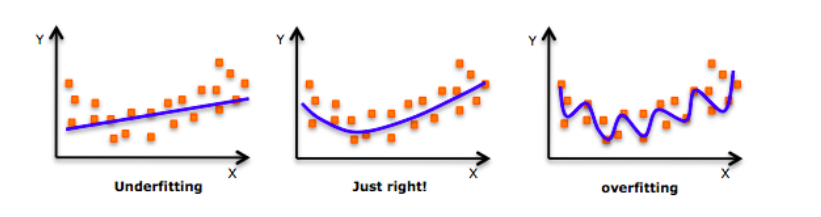
\includegraphics[scale=0.6]{./Figures/Ch_2_Background/Fig_Fitting.png}
\caption{Comparison Between different fitting types}~\label{Fig:Fitting}
\end{figure}%
%
We can enhance the results on testing data by getting more sample data. Therefore, the model can learn the pattern from the data in a better way, but sometimes it is difficult to acquire more data, or it is more expensive than the enhancement required. Hence, we work to apply regularization techniques to prevent overfitting.

Regularization is a technique which applies slight changes or modifications to the algorithm to be more generalized. Sometimes we try to hide information or add noise on the training data to avoid overfitting in the training phase. This considerably improves the model performance in the testing data or unseen.

\paragraph{Different Regularization Techniques in Deep Learning}

In this part, we explain how to apply different regularization techniques in deep learning.

\begin{itemize}
\item \textbf{L2 \& L1 Regularization} are the most common types of regularization. They update the general cost function by adding another term~\eqref{eq:regularization} known as the regularization term~\cite{Web_Analyticsvidhya_Regularization}.
\begin{equation}\label{eq:regularization}
J(w,b) = \ell(y,\widehat{y}) + Regularization
\end{equation}
%
Addition of this regularization term decreases the values of weight matrices. This happens because it assumes that a neural network with smaller weight matrices leads to simpler models. Therefore, it will also reduce overfitting to a significant extent. Assuming we reduce the value of $\lambda$ to be close to zero, this will produce a simpler network and many nodes will be equal zeros. This will reduce the high variance  and hence be less prone to overfitting.%
\begin{enumerate}
\item L2 regularization is the most common type of regularization. In L2 regularization we add $\lambda$ as regularization parameter. This  hyperparameter value is optimized for better results~\eqref{eq:regularization_l2}. It also known as weight decay as it forces the weights to decay towards zero (but not exactly zero)~\cite{Web_Analyticsvidhya_Regularization}.%
\begin{equation}\label{eq:regularization_l2}
J(w,b) = \frac{1}{m} \sum_{i=1}^{m} \ell(y,\widehat{y})+\frac{\lambda}{2m} \times \lVert w \rVert^2
\end{equation}%
\item In L1 Regularization, We penalize the absolute value of the weights~\eqref{eq:regularization_l1}. If we use L1 regularization $W$ can end up being sparse which means $w$ vector will have a lot of zeros. This can help to compress the model because the set of parameters are zero and we need less memory to store the model. Otherwise, we usually prefer L2 over it.%
\begin{equation}\label{eq:regularization_l1}
J(w,b) = \frac{1}{m} \sum_{i=1}^{m} \ell(y,\widehat{y})+\frac{\lambda}{2m} \times \lVert w \rVert
\end{equation}
   \end{enumerate}
  \item \textbf{Dropout}
Dropout is one of the most powerful techniques to apply regularization. It produces excellent results and is consequently the most frequently used regularization technique in the field of deep learning.

Figure~\ref{Fig:NN_Dropout} shows the idea of dropout; it randomly selects some nodes and removes them along with all of their incoming and outgoing connections. Dropout technique’s randomness makes the models’ results seem a more generalized model. For each node, we have a probability of some dropout percentage that this node will be removed with its connections. Therefore, we have some simpler network architecture. Also, dropout forces the algorithm not to rely on any feature. Hence, one must spread the weights and make the network try to learn a different type of features. Therefore, dropout is usually preferred when we have a large neural network structure in order to introduce more randomness.%
%
\begin{figure}[!ht]
	\centering
	\begin{tikzpicture}

	\node[circle, draw, thick] (i1) {};
	\node[circle, draw, thick, above=2em of i1] (i2) {};
	\node[circle, draw, thick, above=2em of i2] (i3) {};
	\node[circle, draw, thick, below=2em of i1] (i4) {};
	\node[circle, draw, thick, below=2em of i4] (i5) {};
	
	\node[circle, draw, thick, right=4em of i1] (h1) {};
	\node[circle, draw, thick, right=4em of i2] (h2) {};
	\node[circle, draw, thick, right=4em of i3] (h3) {};
	\node[circle, draw, thick, right=4em of i4] (h4) {};
	\node[circle, draw, thick, right=4em of i5] (h5) {};
	
	\node[circle, draw, thick, right=4em of h1] (hh1) {};
	\node[circle, draw, thick, right=4em of h2] (hh2) {};
	\node[circle, draw, thick, right=4em of h3] (hh3) {};
	\node[circle, draw, thick, right=4em of h4] (hh4) {};
	\node[circle, draw, thick, right=4em of h5] (hh5) {};
	
	\node[circle, draw, thick, right=4em of hh2] (o1) {};
	\node[circle, draw, thick, right=4em of hh4] (o2) {};
	
	\draw[-stealth, thick] (i1) -- (h1);
	\draw[-stealth, thick] (i1) -- (h2);
	\draw[-stealth, thick] (i1) -- (h3);
	\draw[-stealth, thick] (i1) -- (h4);
	\draw[-stealth, thick] (i1) -- (h5);
	\draw[-stealth, thick] (i2) -- (h1);
	\draw[-stealth, thick] (i2) -- (h2);
	\draw[-stealth, thick] (i2) -- (h3);
	\draw[-stealth, thick] (i2) -- (h4);
	\draw[-stealth, thick] (i2) -- (h5);
	\draw[-stealth, thick] (i3) -- (h1);
	\draw[-stealth, thick] (i3) -- (h2);
	\draw[-stealth, thick] (i3) -- (h3);
	\draw[-stealth, thick] (i3) -- (h4);
	\draw[-stealth, thick] (i3) -- (h5);
	\draw[-stealth, thick] (i4) -- (h1);
	\draw[-stealth, thick] (i4) -- (h2);
	\draw[-stealth, thick] (i4) -- (h3);
	\draw[-stealth, thick] (i4) -- (h4);
	\draw[-stealth, thick] (i4) -- (h5);
	\draw[-stealth, thick] (i5) -- (h1);
	\draw[-stealth, thick] (i5) -- (h2);
	\draw[-stealth, thick] (i5) -- (h3);
	\draw[-stealth, thick] (i5) -- (h4);
	\draw[-stealth, thick] (i5) -- (h5);
	
	\draw[-stealth, thick] (h1) -- (hh1);
	\draw[-stealth, thick] (h1) -- (hh2);
	\draw[-stealth, thick] (h1) -- (hh3);
	\draw[-stealth, thick] (h1) -- (hh4);
	\draw[-stealth, thick] (h1) -- (hh5);
	\draw[-stealth, thick] (h2) -- (hh1);
	\draw[-stealth, thick] (h2) -- (hh2);
	\draw[-stealth, thick] (h2) -- (hh3);
	\draw[-stealth, thick] (h2) -- (hh4);
	\draw[-stealth, thick] (h2) -- (hh5);
	\draw[-stealth, thick] (h3) -- (hh1);
	\draw[-stealth, thick] (h3) -- (hh2);
	\draw[-stealth, thick] (h3) -- (hh3);
	\draw[-stealth, thick] (h3) -- (hh4);
	\draw[-stealth, thick] (h3) -- (hh5);
	\draw[-stealth, thick] (h4) -- (hh1);
	\draw[-stealth, thick] (h4) -- (hh2);
	\draw[-stealth, thick] (h4) -- (hh3);
	\draw[-stealth, thick] (h4) -- (hh4);
	\draw[-stealth, thick] (h4) -- (hh5);
	\draw[-stealth, thick] (h5) -- (hh1);
	\draw[-stealth, thick] (h5) -- (hh2);
	\draw[-stealth, thick] (h5) -- (hh3);
	\draw[-stealth, thick] (h5) -- (hh4);
	\draw[-stealth, thick] (h5) -- (hh5);
	
	
	\draw[-stealth, thick] (hh1) -- (o1);
	\draw[-stealth, thick] (hh1) -- (o2);
	\draw[-stealth, thick] (hh2) -- (o1);
	\draw[-stealth, thick] (hh2) -- (o2);
	\draw[-stealth, thick] (hh3) -- (o1);
	\draw[-stealth, thick] (hh3) -- (o2);
	\draw[-stealth, thick] (hh4) -- (o1);
	\draw[-stealth, thick] (hh4) -- (o2);
	\draw[-stealth, thick] (hh5) -- (o1);
	\draw[-stealth, thick] (hh5) -- (o2);
	
	\draw[-stealth, dashed, thick] (5.5,0) -- node[above] {dropout} (8, 0);
	
	
	%%% BOUNDARY %%%
	
	\node[circle, draw, thick, red, fill=red!10, right=15em of hh1] (i1) {};
	\node[circle, draw, thick, red, fill=red!10, above=2em of i1] (i2) {};
	\node[circle, draw, thick, above=2em of i2] (i3) {};
	\node[circle, draw, thick, below=2em of i1] (i4) {};
	\node[circle, draw, thick, below=2em of i4] (i5) {};
	
	\node[red] (icr) at (i1) {$\mathlarger{\mathlarger{\mathlarger{\mathlarger{\mathlarger{\bm{\times}}}}}}$};
	\node[red] (icr) at (i2) {$\mathlarger{\mathlarger{\mathlarger{\mathlarger{\mathlarger{\bm{\times}}}}}}$};
	
	\node[circle, draw, thick, red, fill=red!10, right=4em of i1] (h1) {};
	\node[circle, draw, thick, right=4em of i2] (h2) {};
	\node[circle, draw, thick, red, fill=red!10, right=4em of i3] (h3) {};
	\node[circle, draw, thick, red, fill=red!10, right=4em of i4] (h4) {};
	\node[circle, draw, thick, right=4em of i5] (h5) {};
	
	\node[red] (icr) at (h1) {$\mathlarger{\mathlarger{\mathlarger{\mathlarger{\mathlarger{\bm{\times}}}}}}$};
	\node[red] (icr) at (h3) {$\mathlarger{\mathlarger{\mathlarger{\mathlarger{\mathlarger{\bm{\times}}}}}}$};
	\node[red] (icr) at (h4) {$\mathlarger{\mathlarger{\mathlarger{\mathlarger{\mathlarger{\bm{\times}}}}}}$};
	
	\node[circle, draw, thick, right=4em of h1] (hh1) {};
	\node[circle, draw, thick, red, fill=red!10, right=4em of h2] (hh2) {};
	\node[circle, draw, thick, right=4em of h3] (hh3) {};
	\node[circle, draw, thick, red, fill=red!10, right=4em of h4] (hh4) {};
	\node[circle, draw, thick, right=4em of h5] (hh5) {};
	
	\node[red] (icr) at (hh2) {$\mathlarger{\mathlarger{\mathlarger{\mathlarger{\mathlarger{\bm{\times}}}}}}$};
	\node[red] (icr) at (hh4) {$\mathlarger{\mathlarger{\mathlarger{\mathlarger{\mathlarger{\bm{\times}}}}}}$};
	
	\node[circle, draw, thick, right=4em of hh2] (o1) {};
	\node[circle, draw, thick, right=4em of hh4] (o2) {};
	
	\draw[-stealth, thick] (i3) -- (h2);
	\draw[-stealth, thick] (i3) -- (h5);
	\draw[-stealth, thick] (i4) -- (h2);
	\draw[-stealth, thick] (i4) -- (h5);
	\draw[-stealth, thick] (i5) -- (h2);
	\draw[-stealth, thick] (i5) -- (h5);
	
	\draw[-stealth, thick] (h2) -- (hh1);
	\draw[-stealth, thick] (h2) -- (hh3);
	\draw[-stealth, thick] (h2) -- (hh5);
	\draw[-stealth, thick] (h5) -- (hh1);
	\draw[-stealth, thick] (h5) -- (hh3);
	\draw[-stealth, thick] (h5) -- (hh5);
	
	\draw[-stealth, thick] (hh1) -- (o1);
	\draw[-stealth, thick] (hh1) -- (o2);
	\draw[-stealth, thick] (hh3) -- (o1);
	\draw[-stealth, thick] (hh3) -- (o2);
	\draw[-stealth, thick] (hh5) -- (o1);
	\draw[-stealth, thick] (hh5) -- (o2);

\end{tikzpicture}

	\caption{A diagram demonstrating the effects of applying dropout with p = 0.5 to a deep neural networks~\cite{Gitrepo_NN_Tikz}}~\label{Fig:NN_Dropout}
\end{figure}%
\item \textbf{Data Augmentation} is a technique to augment your training data when there is no way to acquire more data for the more generalized model. Assuming we are working on Image classifier problem, for example, we can flip the images horizontally and also add that to the training set. Now, instead of this one example in our training set, we can add this to our training example. So by flipping the images horizontally, we could double the size of our training set. Also, we can do different techniques such as rotating the image, flipping, scaling, and shifting the images. All of these techniques can help to produce a better-generalized model.%

\item \textbf{Early stopping} is a type of cross-validation technique where we split some of our training data to be set as the validation set. When we show that our performance on the validation set is getting worse, we immediately stop the training on the model. This is known as early stopping.%@@@ add figure example of early stopping

\end{itemize}

After finalizing this part, we need to note that: In our problem based on text, we found the most effective regularization technique was \textit{Dropout}. After we applied the dropout in our experiments most of the results increased by at least 1\%, and some of the experiments increased by 3.5\%.

\subsubsection{Optimization Algorithms}
As explained previously, we used Gradient Descent algorithm to find the minimum loss for our functions. However, Gradient Descent is not the only algorithm used for this purpose. In this section, we introduce another type of optimization algorithm, most commonly used for optimization problems particular to Deep Learning, named \textit{ADAM Optimization Algorithm}.

\paragraph{ADAM Optimization Algorithm}
ADAM stands for adaptive moment estimation. It is an adaptive learning rate optimization algorithm designed for training deep neural networks, published in 2014 at ICLR 2015~\cite{Adam_2014}. It is one of the best-designed algorithms for deep learning and proven to work well across a wide range of deep learning architectures. The Adam optimization algorithm takes Stochastic Gradient Descent with momentum (it uses a moving average of the gradient instead of gradient itself) and RMS prop (it uses the squared gradients to scale the learning rate) and puts them together. It derives its name from adaptive moment estimation, because Adam uses estimations. The first is $\beta_1$, computing the mean of the derivatives as the first moment. Second, $\beta_2$ is used to compute the exponentially weighted average of the squares and is called the second moment. We can show the algorithm pseudocode in Algorithm~\ref{Alg:Adam}. The chosen Hyperparameter can be as follows:

\begin{enumerate}
\item $\alpha$ is the learning parameter and must be tuned based on the problem type.
\item $\beta_1$ the default choice is 0.9. This is the moving averages in momentum term for (dw,db).
\item $\beta_2$ The author of the Adam paper recommends $0.999$; this computes the moving average of $dw^2$ and $db^2$ squares.
\item $\epsilon$ The author of the Adam paper recommends $10^{-8}$.
\end{enumerate}%

\begin{algorithm}
\caption{ADAM Algorithm for Deep Learning Optimization.}\label{Alg:Adam}
\begin{algorithmic}
  \State Vdw = 0, Sdw = 0, Vdb = 0, Sdb = 0
  \For {$t=0$ to $num\_iterations$} \Comment{\%: compute dw,db on mini-batches}
  \State $V_{dw} = \beta_1 V_{dw} + (1-\beta_1) dw,$\quad$ V_{db} = \beta_1 V_{db} + (1-\beta_1) db$ \Comment{\%:Momentum Step}
  \State $S_{dw} = \beta_2 S_{dw} + (1-\beta_2) dw^2,\quad S_{db} = \beta_2 S_{db} + (1-\beta_2) db$ \Comment{\%:RMS prop Step)}
  \State $V_{dw}^{corrected} = \frac{V_{dw}}{1-\beta_1^t} ,\quad V_{db}^{corrected} = \frac{V_{db}}{1-\beta_1^t} $
  \State $S_{dw}^{corrected} = \frac{S_{dw}}{1-\beta_1^t} ,\quad S_{db}^{corrected} = \frac{S_{db}}{1-\beta_1^t} $
  \State $w:= w-\alpha \frac{V_{dw}^{corrected}}{\sqrt{S_{dw}^{corrected}} + \epsilon},\quad b:= b-\alpha \frac{V_{db}^{corrected}}{\sqrt{S_{db}^{corrected}} + \epsilon}$
  \EndFor
\end{algorithmic}
\end{algorithm}

\subsection{Recurrent Neural Networks (RNNs)}\label{Sec:RNN}

Deep Neural Networks shows its ability to solve many problems. However, in some use cases, Naive Neural Network architecture cannot work or achieve the expected results. One of the famous examples related to this issue in the NLP tasks when working on a text problem. For example, if we say Harry is the king and Elizabeth is the queen, and we need our model to understand from the sentence that, Harry is he and Elizabeth is she. Also, if this word appears again, we need the model to detect that Harry is a person.

This type of problem has a dependency on the input text and how to calculate the output prediction based on the information  provided from the input.

As explained previously, most of the research in this area tries to simulate human brains, so we rarely find anyone trying to think about something start from scratch; it always starts from another related point; for example, what does a human do if he tries to connect the information to generate knowledge about something?

RNN shows its ability to work on sequence data and its related application problems such as natural language\cite{Mikolov_et_al}. The effectiveness of RNN on language modeling is apparent. There are many problems based on this idea of dependency. For example:
\begin{itemize}
\item Time series anomaly detection.
\item Speech recognition.
\item Music composition.
\item Image captioning.
\item Stock market prediction.
\item Translation.
\end{itemize}
So, what are the problems in the Naive Neural Network architecture?
\begin{itemize}
\item Input and output can be different lengths in different examples.
\item The most important issue is that the Naive architecture cannot share features learned across different positions of text. In this case, we lose the learned feature; and the lake of dependency, in this case, affects the overall performance.
\end{itemize}
What is the new proposed architecture which can provide a way to share the features between the Network?
\begin{itemize}
\item First, assuming we have input features $x_1, x_2, x_n$ in the old architecture, we input all these features to the Neural Network, but now we input for example $x_1$ and take the output activation from $a^{<1>}$ to be a feature input with $x_2$, then take the output activation from $a^{<2>}$ as input to $x_3$, similar to $x_n$. figure~\ref{Fig:RNN_Rolled_Loop} shows an example. Hence, this new change allows us to share the learned feature between the networks input data. ,We can also think about it as multiple copies of the same network, each passing a message to a successor\cite{colah}.%

\begin{figure}[!ht]
\minipage{\textwidth}
\centering
\begin{tikzpicture}[scale=2]

% The grid
%  \draw[step=0.5, gray!40, very thin] (-1,-1) grid (8,8);

% LSTM frame
\def \yONE {0.75}

\def \sigmoidWidth  {0.5}
\def \sigmoidInDist {0.2}
\def \sigmoidHeight  {0.5}
\def \yB  {1.5}
\def \yD  {2.75}
\def \xZERO  {0}
\def \xONE  {2}
\def \xTWO  {3.5}
\def \xTHREE  {5}
\def \xFOUR  {7}
\def \shift {1}
\def \bigR {0.25cm}
%%%%%%%%%%%%%%%%%%%%%first one 
% First Sigmoid
\draw[fill=LightYellow] (\xONE, \yB) rectangle (\xONE+ \sigmoidWidth, \yB + \sigmoidHeight) node[pos=0.5] {\Large$\sigma$};
% Upper Arrow Sigmoid 
\draw[arrows=-latex, line width=2.5pt]  (\xONE + \sigmoidWidth/2, \yB +\sigmoidHeight) -- (\xONE + \sigmoidWidth/2, 2.6);
% Circle X_{t+1}
\draw[thick,fill=LightBlue1] (\xONE + \sigmoidWidth/2, \yONE ) circle (\bigR) node {\Large$x_0$};
% Down Arrow X_{t+1}
\draw[arrows=-latex,line width=2.5pt] (\xONE + \sigmoidWidth/2, \yONE + 0.25)  --  (\xONE + \sigmoidWidth/2, \yB);
% Circle H{t} 
\draw[thick,fill=LightPurple1] (\xONE + \sigmoidWidth/2, \yD) circle (\bigR) node {\Large$h_0$};
% Right Arrow H{t} 
\draw[arrows=-latex, line width=2.5pt] (\xONE + \sigmoidWidth/2+\sigmoidWidth/2, 1.75)   
--  (\xTWO, 1.75)
node[right, xshift=-0.9cm, yshift=0.4cm,] {\Large$h_0$};
%%%%%%%%%%%%%%%%%%%%%second one 
% First Sigmoid
%%%%%%%%%%%%%%%%%%%%%first one 
% First Sigmoid
\draw[fill=LightYellow] (\xTWO, \yB) rectangle (\xTWO+ \sigmoidWidth, \yB + \sigmoidHeight) node[pos=0.5] {\Large$\sigma$};
% Upper Arrow Sigmoid 
\draw[arrows=-latex, line width=2.5pt]  (\xTWO + \sigmoidWidth/2, \yB +\sigmoidHeight) -- (\xTWO + \sigmoidWidth/2, 2.6);
% Circle X_{t+1}
\draw[thick,fill=LightBlue1] (\xTWO + \sigmoidWidth/2, \yONE ) circle (\bigR) node {\Large$x_1$};
% Down Arrow X_{t+1}
\draw[arrows=-latex,line width=2.5pt] (\xTWO + \sigmoidWidth/2, \yONE + 0.25)  --  (\xTWO + \sigmoidWidth/2, \yB);
% Circle H{t} 
\draw[thick,fill=LightPurple1] (\xTWO + \sigmoidWidth/2, \yD) circle (\bigR) node {\Large$h_1$};
% Right Arrow H{t} 
\draw[arrows=-latex, line width=2.5pt] (\xTWO + \sigmoidWidth/2+\sigmoidWidth/2, 1.75)   
--  (\xTHREE, 1.75)
node[right, xshift=-0.9cm, yshift=0.4cm,] {\Large$h_1$};

%%%%%%%%%%%%%%%%%%%%%first one 
% First Sigmoid
\draw[fill=LightYellow] (\xTHREE, \yB) rectangle (\xTHREE+ \sigmoidWidth, \yB + \sigmoidHeight) node[pos=0.5] {\Large$\sigma$};
% Upper Arrow Sigmoid 
\draw[arrows=-latex, line width=2.5pt]  (\xTHREE + \sigmoidWidth/2, \yB +\sigmoidHeight) -- (\xTHREE + \sigmoidWidth/2, 2.6);
% Circle X_{t+1}
\draw[thick,fill=LightBlue1] (\xTHREE + \sigmoidWidth/2, \yONE ) circle (\bigR) node {\Large$x_2$};
% Down Arrow X_{t+1}
\draw[arrows=-latex,line width=2.5pt] (\xTHREE + \sigmoidWidth/2, \yONE + 0.25)  --  (\xTHREE + \sigmoidWidth/2, \yB);
% Circle H{t} 
\draw[thick,fill=LightPurple1] (\xTHREE + \sigmoidWidth/2, \yD) circle (\bigR) node {\Large$h_2$};
% Right Arrow H{t} 
\draw[arrows=-latex, line width=2.5pt] (\xTHREE + \sigmoidWidth/2+\sigmoidWidth/2, 1.75)   
--  (\xFOUR, 1.75)
node[right, xshift=-0.9cm, yshift=0.4cm,] {\Large$h_2$};

%%%%%%%%%%%%%%%%%%%%%first one 
% First Sigmoid
\draw[fill=LightYellow] (\xFOUR, \yB) rectangle (\xFOUR+ \sigmoidWidth, \yB + \sigmoidHeight) node[pos=0.5] {\Large$\sigma$};
% Upper Arrow Sigmoid 
\draw[arrows=-latex, line width=2.5pt]  (\xFOUR + \sigmoidWidth/2, \yB +\sigmoidHeight) -- (\xFOUR + \sigmoidWidth/2, 2.6);
% Circle X_{t+1}
\draw[thick,fill=LightBlue1] (\xFOUR + \sigmoidWidth/2, \yONE ) circle (\bigR) node {\Large$x_{t}$};
% Down Arrow X_{t+1}
\draw[arrows=-latex,line width=2.5pt] (\xFOUR + \sigmoidWidth/2, \yONE + 0.25)  --  (\xFOUR + \sigmoidWidth/2, \yB);
% Circle H{t} 
\draw[thick,fill=LightPurple1] (\xFOUR + \sigmoidWidth/2, \yD) circle (\bigR) node {\Large$h_t$};
% Right Arrow H{t} 
\draw[arrows=-latex, line width=2.5pt] (\xFOUR + \sigmoidWidth/2+\sigmoidWidth/2, 1.75)   
--  (\xFOUR + \sigmoidWidth + \sigmoidWidth, 1.75)
node[right, xshift=-0.9cm, yshift=0.4cm,] {\Large$h_t$};
\node[text width=1cm] at (\xFOUR-.75,1) 
{\LARGE....};

%%%%%%%%%%%%%%%%%%%%%first one 
% First Sigmoid
\draw[fill=LightYellow] (\xZERO, \yB) rectangle (\xZERO+ \sigmoidWidth, \yB + \sigmoidHeight) node[pos=0.5] {\Large$\sigma$};
% Upper Arrow Sigmoid 
\draw[arrows=-latex, line width=2.5pt]  (\xZERO + \sigmoidWidth/2, \yB +\sigmoidHeight) -- (\xZERO + \sigmoidWidth/2, 2.6);
% Circle X_{t+1}
\draw[thick,fill=LightBlue1] (\xZERO + \sigmoidWidth/2, \yONE ) circle (\bigR) node {\Large$x_0$};
% Down Arrow X_{t+1}
\draw[arrows=-latex,line width=2.5pt] (\xZERO + \sigmoidWidth/2, \yONE + 0.25)  --  (\xZERO + \sigmoidWidth/2, \yB);
% Circle H{t} 
\draw[thick,fill=LightPurple1] (\xZERO + \sigmoidWidth/2, \yD) circle (\bigR) node {\Large$h_0$};
% Right Arrow H{t} 
\draw[line width=2.5pt] (\xZERO + \sigmoidWidth/2+\sigmoidWidth/2, 1.75)   
--  (.5+\sigmoidWidth/2, 1.75);

\draw[line width=2.5pt] (.5+\sigmoidWidth/2, 1.73)   
--  (.5+\sigmoidWidth/2, 2.25);

\draw[line width=2.5pt] (.5+\sigmoidWidth/2, 2.23)   
--  (\xZERO + \sigmoidWidth/2+.03, 2.23);

\draw[line width=2.5pt] (\xZERO + \sigmoidWidth/2-.03, 2.23)   
--  (\xZERO - \sigmoidWidth/2, 2.23);

\draw[line width=2.5pt] (\xZERO - \sigmoidWidth/2, 2.25)
--  (\xZERO - \sigmoidWidth/2, 1.75);

\draw[arrows=-latex,line width=2.5pt] (\xZERO-.02 - \sigmoidWidth/2, 1.75)
--  (\xZERO , 1.75);

\node[text width=1cm] at (1.5,1.75) {\LARGE=};
\end{tikzpicture}

\endminipage\hfill
\caption{Recurrent Neural Networks Loops adapted from~\cite{colah}}\label{Fig:RNN_Rolled_Loop}
\minipage{0.33\textwidth}
\begin{tikzpicture}[scale=1.45]


% The grid
% \draw[step=0.5, gray!40, very thin] (0,0) grid (8,4);

% LSTM frame
\def \yONE {0.5}
\def \yTWO {3.3}
\draw[rounded corners=10pt, very thick, fill=LightGreen]  (1.5, 0.5) rectangle (5, 2.3);

\def \sigmoidWidth  {0.45}
\def \sigmoidInDist {0.2}
\def \sigmoidHeight  {0.3}
\def \yB  {1.3}
\def \yD  {2}
\def \shift {0.3}
\def \bigR {0.25cm}
\def \C    {1}
\def \xBigCicleONE {2}
\def \xBigCicleTWO {5.5 + 0.25}
\def \levelB {1}

% Second times operator and add operator
\def \xTimesB {2.6}
\def \yC      {1}
\def \xOfThirdSigmoid {\xSSS + \sigmoidWidth/2}


% Square tanh
\draw[fill=LightYellow]  (3,1.5-\sigmoidHeight/2) 
rectangle 
(3 +\sigmoidWidth, 1.5-\sigmoidHeight/2 +\sigmoidHeight)
node[pos=0.5] {\scriptsize\textit{tanh}};

%tanh upper line
\draw[line width=2.5pt,gray]  (3.2,1.65) -- (3.2, \yD);


%line A upper left input from previous cell
%\draw[arrows=-latex,line width=2.5pt,gray]  (1, \yD) -- (1.5, \yD);

%line A upper left input after cell
\draw[line width=2.5pt,gray]  (1.5, \yD) -- (2.4, \yD);

\draw[arrows=-latex, line width=2.5pt,gray] (2.39, \yD)  to[out=270, in=180] (3,1.5);

%line A upper from tanh to rictangle border
\draw[line width=2.5pt,gray]  (3.2, \yD) -- (5, \yD);

%line A upper from rictangle border to next cell
\draw[arrows=-latex,line width=2.5pt]  (5, \yD) -- (5.5, \yD);


%level B line 
\draw[line width=2.5pt,gray] (2.2, \levelB) 
--
(2.4, \levelB);

%second line last angle connected to sigmoid 

\draw[arrows=-latex, line width=2.5pt,gray] (2.39,1) 
to[out=90, in=180] 
(3,1.5);



\draw[thick,fill=LightBlue] (\xBigCicleONE, \yONE+.4 - \C) circle (\bigR) node {$x_{t-1}$};

% x_t line
\draw[line width=2.5pt,gray] (\xBigCicleONE, \yONE -\C +0.65) 
--
(\xBigCicleONE, \yONE -\C +0.25 + 1.1);

\draw[line width=2.5pt,gray] (\xBigCicleONE, \yONE -\C +0.25 + 1.1)
to[out=90, in=180]
(2.25, 1);


\draw[thick,fill=LightPurple] (\xBigCicleTWO-1, \yTWO -1.15 + \C) circle (\bigR) node {$h_{t-1}$};
%h_T lines
\draw[arrows=-latex, line width=2.5pt,gray]
(\xBigCicleTWO-1, \yD )
--
(\xBigCicleTWO-1, \yTWO -1.4 + \C);


\end{tikzpicture}

\endminipage\hfill
\minipage{0.33\textwidth}
\begin{tikzpicture}[scale=1.45]


% The grid
% \draw[step=0.5, gray!40, very thin] (0,0) grid (8,4);

% LSTM frame
\def \yONE {0.5}
\def \yTWO {3.3}
\draw[rounded corners=10pt, very thick, fill=LightGreen]  (1.5, 0.5) rectangle (5, 2.3);

\def \sigmoidWidth  {0.45}
\def \sigmoidInDist {0.2}
\def \sigmoidHeight  {0.3}
\def \yB  {1.3}
\def \yD  {2}
\def \shift {0.3}

% Square tanh
\draw[fill=LightYellow]  (3,1.5-\sigmoidHeight/2) 
rectangle 
(3 +\sigmoidWidth, 1.5-\sigmoidHeight/2 +\sigmoidHeight)
node[pos=0.5] {\scriptsize\textit{tanh}};

%tanh upper line
\draw[line width=2.5pt]  (3.2,1.65) -- (3.2, \yD);

% Second times operator and add operator
\def \xTimesB {2.6}
\def \yC      {1}

%line A upper left input from previous cell
%\draw[arrows=-latex,line width=2.5pt]  (1, \yD) -- (1.5, \yD);

%line A upper left input after cell
\draw[line width=2.5pt]  (1.5, \yD) -- (2.4, \yD);

\draw[arrows=-latex, line width=2.5pt] (2.39, \yD)  to[out=270, in=180] (3,1.5);

%line A upper from tanh to rictangle border
\draw[line width=2.5pt]  (3.2, \yD) -- (5, \yD);

%line A upper from rictangle border to next cell
\draw[arrows=-latex,line width=2.5pt]  (5, \yD) -- (5.5, \yD);


\def \levelB {1}
%level B line 
\draw[line width=2.5pt] (2.2, \levelB) 
--
(2.4, \levelB);

\def \xOfThirdSigmoid {\xSSS + \sigmoidWidth/2}
%second line last angle connected to sigmoid 

\draw[arrows=-latex, line width=2.5pt] (2.39,1) 
to[out=90, in=180] 
(3,1.5);


\def \bigR {0.25cm}
\def \bigRTWO {0.4cm}
\def \C    {1}
\def \xBigCicleONE {2}
\def \xBigCicleTWO {5.5 + 0.25}

\draw[thick,fill=LightBlue] (\xBigCicleONE, \yONE+.4 - \C) circle (\bigR) node {$x_{t}$};

% x_t line
\draw[line width=2.5pt] (\xBigCicleONE, \yONE -\C +0.65) 
--
(\xBigCicleONE, \yONE -\C +0.25 + 1.1);

\draw[line width=2.5pt] (\xBigCicleONE, \yONE -\C +0.25 + 1.1)
to[out=90, in=180]
(2.25, 1);



\draw[thick,fill=LightPurple] (\xBigCicleTWO-1, \yTWO -1.15 + \C) circle (\bigR) node {$h_{t}$};
%h_T lines
\draw[arrows=-latex, line width=2.5pt]
(\xBigCicleTWO-1, \yD )
--
(\xBigCicleTWO-1, \yTWO -1.4 + \C);


\end{tikzpicture}

\endminipage\hfill
\minipage{0.33\textwidth}%
\begin{tikzpicture}[scale=1.45]


% The grid
% \draw[step=0.5, gray!40, very thin] (0,0) grid (8,4);

% LSTM frame
\def \yONE {0.5}
\def \yTWO {3.3}
\draw[rounded corners=10pt, very thick, fill=LightGreen]  (1.5, 0.5) rectangle (5, 2.3);

\def \sigmoidWidth  {0.45}
\def \sigmoidInDist {0.2}
\def \sigmoidHeight  {0.3}
\def \yB  {1.3}
\def \yD  {2}
\def \shift {0.3}
\def \bigRTWO {0.4cm}
% Square tanh
\draw[fill=LightYellow]  (3,1.5-\sigmoidHeight/2) 
rectangle 
(3 +\sigmoidWidth, 1.5-\sigmoidHeight/2 +\sigmoidHeight)
node[pos=0.5] {\scriptsize\textit{tanh}};

%tanh upper line
\draw[line width=2.5pt,gray]  (3.2,1.65) -- (3.2, \yD);

% Second times operator and add operator
\def \xTimesB {2.6}
\def \yC      {1}

%line A upper left input from previous cell
%\draw[arrows=-latex,line width=2.5pt]  (1, \yD) -- (1.5, \yD);

%line A upper left input after cell
\draw[line width=2.5pt,gray]  (1.5, \yD) -- (2.4, \yD);

\draw[arrows=-latex, line width=2.5pt,gray] (2.39, \yD)  to[out=270, in=180] (3,1.5);

%line A upper from tanh to rictangle border
\draw[line width=2.5pt,gray]  (3.2, \yD) -- (5, \yD);

%line A upper from rictangle border to next cell
\draw[arrows=-latex,line width=2.5pt]  (5, \yD) -- (5.6, \yD);


\def \levelB {1}
%level B line 
\draw[line width=2.5pt,gray] (2.2, \levelB) 
--
(2.4, \levelB);

\def \xOfThirdSigmoid {\xSSS + \sigmoidWidth/2}
%second line last angle connected to sigmoid 

\draw[arrows=-latex, line width=2.5pt,gray] (2.39,1) 
to[out=90, in=180] 
(3,1.5);


\def \bigR {0.25cm}
\def \C    {1}
\def \xBigCicleONE {2}
\def \xBigCicleTWO {5.5 + 0.25}

\draw[thick,fill=LightBlue] (\xBigCicleONE, \yONE+.4 - \C) circle (\bigR) node {$x_{t+1}$};

% x_t line
\draw[line width=2.5pt,gray] (\xBigCicleONE, \yONE -\C +0.65) 
--
(\xBigCicleONE, \yONE -\C +0.25 + 1.1);

\draw[line width=2.5pt,gray] (\xBigCicleONE, \yONE -\C +0.25 + 1.1)
to[out=90, in=180]
(2.25, 1);



\draw[thick,fill=LightPurple] (\xBigCicleTWO-1, \yTWO -1.15 + \C) circle (\bigR) node {$h_{t+1}$};
%h_T lines
\draw[arrows=-latex, line width=2.5pt,gray]
(\xBigCicleTWO-1, \yD )
--
(\xBigCicleTWO-1, \yTWO -1.4 + \C);


\end{tikzpicture}

\endminipage
\caption{The repeating module in a standard RNN containing a single layer adapted from~\cite{colah}}~\label{Fig:LSTM_SimpleRNN}

\end{figure}%

\item Second, the feedforward computes for time t and then we calculate the loss at step t. The final loss is the sum of loss at every step; t~\eqref{eq:rnn_feedfarward} explains feedforward steps. The backpropagation is also calculated through time at every step.% 
\begin{subequations}\label{eq:rnn_feedfarward}
\begin{align}
 a^{<t>} & = g(W_{aa}a^{<t-1>}+ W_{ax}x^{<t>}+b_a)\\
  & = g(W_a[a^{<t-1>},x^{<t>}]+ b_a)\\
 \widehat{y}^{<t>} & = g(W_{ya}a^{<t>}+ b_y)
 \\ \ell^{<t>}(\widehat{y}^{<t>},y^{<t>}) & = - (y^{<t>} \log \widehat{y}^{<t>} + (1-y^{<t>}) \log (1-\widehat{y}^{<t>}))
\\ \ell(\widehat{y},y) & = \sim_{t=1}^{T_m} \ell^{<t>}(\widehat{y}^{<t>},y^{<t>})   
\end{align}
\end{subequations}%
 \end{itemize}


 \subsubsection{Vanishing Gradient with RNNs}\label{Sec:RNN_Vanishing}
 
As explained, RNN works on sequential data, and the idea is to predict new output not only based on the input data vector but also, other input vectors. Due to the recurrent structure in RNNs, it tends to suffer from long-term dependency. To simplify this point, consider the following sentence:\\
\textit{Waleed Yousef, who is Associate Professor at Helwan University and teaches Data Science courses and its dependencies, \textbf{\underline{got}} a Ph.D. in Computer Engineering from GWU in 2006.}

In the previous example, predicting the word \underline{got} depends on the sentence’s tense whether it present or past to be consistent is correct. It also shows how some problems need the long-term dependencies handling.[Bengio et al.,1994]~\cite{Bengio_1994} showed that Basic RNNs have a problem in long-term dependency.  Another problem which may happen in basic Neural Networks is gradient exploding. One of the side-effects of gradient exploding is an exponentially large gradient which causes our parameters to be so large. Hence, the Neural Networks parameters have a severe problem. Another serious problem with Basic Neural Networks is overfitting problems [Zaremba et al., 2014]~\cite{Zaremba_et_al}.

To solve this learning problem [Hochreiter and Schmidhuber, 1997] introduced Long Short-Term Memory which helps to reduce the dependency problem using memory cells and forget gates.%
\subsection{Long Short Term Memory networks (LSTMs)}\label{Sec:LSTM}


Long Short Term Memory networks – “LSTMs” – are a special type of RNN, capable of learning long-term dependencies. To solve the vanishing gradient problem for long-term dependencies, [Hochreiter and Schmidhuber, 1997]~\cite{Hochreiter} suggested new cell architecture for RNN by adding Long Short Term Memory which significantly reduced the long-term dependency problem using memory cells and forget gates.

LSTMs are designed to help solving the long-term dependency problem and to hold information in memory for long periods of time. They use the RNNs’ sequential model but add gating mechanism structures to every cell.

Both Basic RNNs and LSTM have the form of a chain of repeating modules of neural network. The main difference is the structure of the Networks.%

Basic RNNs have very simple structure for every layer with simple output function~\ref{Fig:LSTM_SimpleRNN}. However, LSTMs have four interacting layers Figure~\ref{Fig:LSTM_Cell_Chaining}.
\begin{figure}[!ht]
	
	\minipage{0.33\textwidth}
	\begin{tikzpicture}[scale=1.1]

  % The grid
  % \draw[step=0.5, gray!40, very thin] (0,0) grid (8,4);

  % LSTM frame
  \def \yONE {0.5}
  \def \yTWO {3.3}
  \draw[rounded corners=10pt, very thick, gray,fill=LightGreen]  (1.5, 0.5) rectangle (6.2, 3.3);

  \def \sigmoidWidth  {0.45}
  \def \sigmoidInDist {0.2}
  \def \sigmoidHeight  {0.3}
  \def \yB  {1.3}
  \def \yD  {2.75}
  \def \shift {0.3}
  % First Sigmoid
  \draw[gray,fill=LightYellow] (2, \yB) rectangle (2+ \sigmoidWidth, \yB + \sigmoidHeight) node[pos=0.5] {$\sigma$};

  \def \r {.15cm}
  % The Upper times operator % first time from left
  \draw[thick, gray,fill=pink] (2.25, \yD) circle (\r) node {$\times$};

  % Second Sigmoid
  \def \xS {2.45 +\sigmoidInDist}
  \draw[gray,fill=LightYellow]  (\xS, \yB) rectangle (\xS +\sigmoidWidth, \yB + \sigmoidHeight) node[pos=0.5] {$\sigma$};

  % Square tanh
  \def \xSS {\xS +\sigmoidWidth + \sigmoidInDist}
  \draw[gray,fill=LightYellow]  (\xSS, \yB) 
  rectangle 
  (\xSS +\sigmoidWidth +0.13, \yB +\sigmoidHeight)
  node[pos=0.5] {\scriptsize \textit{tanh}};

  % Third Sigoid
  \def \xSSS {\xSS +\sigmoidWidth +0.13 +\sigmoidInDist}
  \draw[gray,fill=LightYellow]  (\xSSS, \yB) rectangle (\xSSS +\sigmoidWidth, \yB +\sigmoidHeight)
  node[pos=0.5] { $\sigma$};

  % Second times operator and add operator
  \def \xTimesB {3.6}
  \def \yC      {2}

  \draw[thick,gray,fill=pink] (\xTimesB, \yC) circle (\r) node {$\times$};
  %%%%% first line sectond operator +
  \draw[thick, gray,fill=pink] (\xTimesB, \yD) circle (\r) node {$+$};

  % Third times operator and its tanh
  \draw[thick,gray,fill=pink] (\xTimesB +1.3 +\shift, \yC) circle (\r) node {$\times$};
  \draw[thick,gray,fill=LightYellow] (\xTimesB +1.3 +\shift, \yC +.4)  
  ellipse (.35cm and .14cm) 
  node {\scriptsize \textit{tanh}};


  % LINES %%% Upper line from c_{t -1} till C_t
  %\draw[arrows=-latex, line width=2.5pt]  (0.85, \yD) -- (1.5, \yD) node[left, xshift=-.6cm, yshift=0.2cm] {$C_{t-1}$};
  \draw[line width=2.5pt, gray]  (1.5, \yD) -- (2.1, \yD);
  \draw[line width=2.5pt, gray]  (2.4, \yD) -- (3.46, \yD);
  \draw[line width=2.5pt,gray]  (3.75, \yD) -- (6.25 +0.2, \yD);

  \draw[arrows=-latex, line width=2.5pt]  (6.25, \yD) -- (6.75 +0.2, \yD)
  node[right, xshift=0.0cm, yshift=0.05cm] {$C_t$};

  %%%%first line from left from sigmoid ft till times input from C_{t-1}
  \draw[arrows=-latex, line width=1.5pt,gray]  (2.25, \yB +\sigmoidHeight) -- (2.25, 2.6)
  node[left, yshift=-0.5cm] {$f_t$};

  % Level B LINES
  \def \levelB {1}
  %\draw[arrows=-latex, line width=1.5pt,gray] (0.85, \levelB) -- (1.5, \levelB) node[left, xshift=-.6cm, yshift=0.2cm] {$h_{t-1}$};

  \draw[line width=1.5pt,gray] (1.5, \levelB) 
  --
  (4.2, \levelB);

  \def \xOfThirdSigmoid {\xSSS + \sigmoidWidth/2}
  %second line last angle connected to sigmoid 
  \draw[line width=1.5pt,gray] (4.2, \levelB) to[out=0,in=270] (\xOfThirdSigmoid, \yB);

  % Third Sigmoid up line
  % END (\xTimesB +1.3 - 0.19 , \yC)
  \draw[line width=1.5pt,gray] (\xOfThirdSigmoid, \yB + \sigmoidHeight) 
  --
  (\xOfThirdSigmoid, \yB + \sigmoidHeight + 0.17) ;

  \draw[arrows=-latex, line width=1.5pt,gray] (\xOfThirdSigmoid, \yB + \sigmoidHeight+0.17) 
  to[out=90, in=180] 
  (\xTimesB +1.3 -0.14 +\shift , \yC) 
  node [left, yshift=0.2cm, xshift=-0.2cm] {$o_t$};

  % tanh line
  \draw [line width=1.5pt,gray] (\xTimesB, \levelB)
  --
  (\xTimesB, \yB);

  \draw [line width=1.5pt,gray] (\xTimesB, \yB + \sigmoidHeight)
  --
  (\xTimesB, \yB + \sigmoidHeight +0.24);

  \draw [arrows=-latex, line width=1.5pt,gray] (\xTimesB, 2.15)
  --
  (\xTimesB, 2.6);

  \draw[line width=1.5pt,gray] (2.25, \levelB)
  --
  (2.25, \yB);
  
  \draw[line width=1.5pt,gray] (\xS +\sigmoidWidth/2, \levelB)
  --
  (\xS +\sigmoidWidth/2, \yB);

  \draw[line width=1.5pt,gray] (\xS +\sigmoidWidth/2, \yB +\sigmoidHeight)
  -- 
  (\xS +\sigmoidWidth/2, \yB +\sigmoidHeight + 0.17);

  \draw[arrows=-latex, line width=1.5pt,gray] (\xS +\sigmoidWidth/2, \yB + \sigmoidHeight+0.17) 
  to[out=90, in=180] 
  (\xTimesB-0.14, \yC)
  node [left, yshift=0.2cm, xshift=-0.2cm] {$i_t$};

  \def \bigR {0.25cm}
  \def \bigRTWO {0.4cm}
  \def \C    {1}
  \def \xBigCicleONE {2}
  \def \xBigCicleTWO {5.5 + 0.25}
  \draw[thick,gray] (\xBigCicleONE, \yONE - \C) circle (\bigRTWO) node {$x_{t-1}$};
  \draw[thick,gray] (\xBigCicleTWO, \yTWO + \C) circle (\bigRTWO) node {$h_{t-1}$};

  % LINE Circle ONE
  \draw[line width=1.5pt,gray] (\xBigCicleONE, \yONE -\C +0.25) 
  --
  (\xBigCicleONE, \yONE -\C +0.25 + 1.1);

  \draw[line width=1.5pt,gray] (\xBigCicleONE, \yONE -\C +0.25 + 1.1)
  to[out=90, in=180]
  (2.25, 1);

  % LINE third \times
  \draw[line width=1.5pt,gray] (\xTimesB +1.3 +\shift, 1.1)
  --
  (\xTimesB +1.3 +\shift, \yC - 0.15);

  \draw[line width=1.5pt,gray] (5.5, 1) 
  --
  (6.25 +0.2, 1);
  
  \draw[arrows=-latex,line width=2.5pt] (6.25, 1) 
  --
  (6.75 +0.2, 1)
  node[right, xshift=0.0cm, yshift=0.05cm,] {$h_t$};

%%% second line last angle connect the input with h_t output
  \draw[line width=1.5pt,gray] (\xTimesB +1.3 +\shift, 1.1)
  to[out=270, in=180]
  (5.5, 1);


  \draw[line width=1.5pt,gray] (\xTimesB +1.3 +\shift, 2.14)
  --
  (\xTimesB +1.3 +\shift, 2.26);


  \draw[line width=1.5pt,gray] (\xTimesB +1.3 +\shift, \yD)
  --
  (\xTimesB +1.3 +\shift, 2.54);


  \draw[line width=1.5pt,gray] (\xBigCicleTWO, \levelB +0.2)
  --
  (\xBigCicleTWO, 2.6);

%%%%% first horizontal line from the right angle connected to output ht
  \draw[line width=1.5pt,gray] (\xBigCicleTWO - 0.2, \levelB)
  to[out=0, in=270]
  (\xBigCicleTWO, \levelB +0.2);


  \draw[arrows=-latex, line width=1.5pt,gray]
  (\xBigCicleTWO, \yD +0.15)
  --
  (\xBigCicleTWO, 4);

\end{tikzpicture}


	\endminipage\hfill
	\minipage{0.33\textwidth}
	\begin{tikzpicture}[scale=1.1]

  % The grid
  % \draw[step=0.5, gray!40, very thin] (0,0) grid (8,4);

  % LSTM frame
  \def \yONE {0.5}
  \def \yTWO {3.3}
  \draw[rounded corners=10pt, very thick, gray,fill=LightGreen]  (1.5, 0.5) rectangle (6.2, 3.3);

  \def \sigmoidWidth  {0.45}
  \def \sigmoidInDist {0.2}
  \def \sigmoidHeight  {0.3}
  \def \yB  {1.3}
  \def \yD  {2.75}
  \def \shift {0.3}
  % First Sigmoid
  \draw[gray,fill=LightYellow] (2, \yB) rectangle (2+ \sigmoidWidth, \yB + \sigmoidHeight) node[pos=0.5] {$\sigma$};

  \def \r {.15cm}
  % The Upper times operator % first time from left
  \draw[thick, gray,fill=pink] (2.25, \yD) circle (\r) node {$\times$};

  % Second Sigmoid
  \def \xS {2.45 +\sigmoidInDist}
  \draw[gray,fill=LightYellow]  (\xS, \yB) rectangle (\xS +\sigmoidWidth, \yB + \sigmoidHeight) node[pos=0.5] {$\sigma$};

  % Square tanh
  \def \xSS {\xS +\sigmoidWidth + \sigmoidInDist}
  \draw[gray,fill=LightYellow]  (\xSS, \yB) 
  rectangle 
  (\xSS +\sigmoidWidth +0.13, \yB +\sigmoidHeight)
  node[pos=0.5] {\scriptsize \textit{tanh}};

  % Third Sigoid
  \def \xSSS {\xSS +\sigmoidWidth +0.13 +\sigmoidInDist}
  \draw[gray,fill=LightYellow]  (\xSSS, \yB) rectangle (\xSSS +\sigmoidWidth, \yB +\sigmoidHeight)
  node[pos=0.5] { $\sigma$};

  % Second times operator and add operator
  \def \xTimesB {3.6}
  \def \yC      {2}

  \draw[thick,fill=pink] (\xTimesB, \yC) circle (\r) node {$\times$};
  %%%%% first line sectond operator +
  \draw[thick, gray,fill=pink] (\xTimesB, \yD) circle (\r) node {$+$};

  % Third times operator and its tanh
  \draw[thick,fill=pink] (\xTimesB +1.3 +\shift, \yC) circle (\r) node {$\times$};
  \draw[thick,fill=LightYellow] (\xTimesB +1.3 +\shift, \yC +.4)  
  ellipse (.35cm and .14cm) 
  node {\scriptsize \textit{tanh}};


  % LINES %%% Upper line from c_{t -1} till C_t
  %\draw[arrows=-latex, line width=2.5pt]  (0.85, \yD) -- (1.5, \yD) node[left, xshift=-.6cm, yshift=0.2cm] {$C_{t-1}$};
  \draw[line width=2.5pt]  (1.5, \yD) -- (2.1, \yD);
  \draw[line width=2.5pt]  (2.4, \yD) -- (3.46, \yD);
  \draw[line width=2.5pt]  (3.75, \yD) -- (6.25 +0.2, \yD);

  \draw[arrows=-latex, line width=2.5pt]  (6.25, \yD) -- (6.75 +0.2, \yD)
  node[right, xshift=0.0cm, yshift=0.05cm] {$C_t$};

  %%%%first line from left from sigmoid ft till times input from C_{t-1}
  \draw[arrows=-latex, line width=2.5pt]  (2.25, \yB +\sigmoidHeight) -- (2.25, 2.6)
  node[left, yshift=-0.5cm] {$f_t$};

  % Level B LINES
  \def \levelB {1}
  %\draw[arrows=-latex, line width=2.5pt] (0.85, \levelB) -- (1.5, \levelB) node[left, xshift=-.6cm, yshift=0.2cm] {$h_{t-1}$};

  \draw[line width=2.5pt] (1.5, \levelB) 
  --
  (4.2, \levelB);

  \def \xOfThirdSigmoid {\xSSS + \sigmoidWidth/2}
  %second line last angle connected to sigmoid 
  \draw[line width=2.5pt] (4.2, \levelB) to[out=0,in=270] (\xOfThirdSigmoid, \yB);

  % Third Sigmoid up line
  % END (\xTimesB +1.3 - 0.19 , \yC)
  \draw[line width=2.5pt] (\xOfThirdSigmoid, \yB + \sigmoidHeight) 
  --
  (\xOfThirdSigmoid, \yB + \sigmoidHeight + 0.17) ;

  \draw[arrows=-latex, line width=2.5pt] (\xOfThirdSigmoid, \yB + \sigmoidHeight+0.17) 
  to[out=90, in=180] 
  (\xTimesB +1.3 -0.14 +\shift , \yC) 
  node [left, yshift=0.2cm, xshift=-0.2cm] {$o_t$};

  % tanh line
  \draw [line width=2.5pt] (\xTimesB, \levelB)
  --
  (\xTimesB, \yB);

  \draw [line width=2.5pt] (\xTimesB, \yB + \sigmoidHeight)
  --
  (\xTimesB, \yB + \sigmoidHeight +0.24);

  \draw [arrows=-latex, line width=2.5pt] (\xTimesB, 2.15)
  --
  (\xTimesB, 2.6);

  \draw[line width=2.5pt] (2.25, \levelB)
  --
  (2.25, \yB);
  
  \draw[line width=2.5pt] (\xS +\sigmoidWidth/2, \levelB)
  --
  (\xS +\sigmoidWidth/2, \yB);

  \draw[line width=2.5pt] (\xS +\sigmoidWidth/2, \yB +\sigmoidHeight)
  -- 
  (\xS +\sigmoidWidth/2, \yB +\sigmoidHeight + 0.17);

  \draw[arrows=-latex, line width=2.5pt] (\xS +\sigmoidWidth/2, \yB + \sigmoidHeight+0.17) 
  to[out=90, in=180] 
  (\xTimesB-0.14, \yC)
  node [left, yshift=0.2cm, xshift=-0.2cm] {$i_t$};

  \def \bigR {0.25cm}
  \def \bigRTWO {0.4cm}
  \def \C    {1}
  \def \xBigCicleONE {2}
  \def \xBigCicleTWO {5.5 + 0.25}
  \draw[thick] (\xBigCicleONE, \yONE - \C) circle (\bigRTWO) node {$x_{t+1}$};
  \draw[thick] (\xBigCicleTWO, \yTWO + \C) circle (\bigRTWO) node {$h_{t+1}$};

  % LINE Circle ONE
  \draw[line width=2.5pt] (\xBigCicleONE, \yONE -\C +0.25) 
  --
  (\xBigCicleONE, \yONE -\C +0.25 + 1.1);

  \draw[line width=2.5pt] (\xBigCicleONE, \yONE -\C +0.25 + 1.1)
  to[out=90, in=180]
  (2.25, 1);

  % LINE third \times
  \draw[line width=2.5pt] (\xTimesB +1.3 +\shift, 1.1)
  --
  (\xTimesB +1.3 +\shift, \yC - 0.15);

  \draw[line width=2.5pt] (5.5, 1) 
  --
  (6.25 +0.2, 1);
  
  \draw[arrows=-latex, line width=2.5pt] (6.25, 1) 
  --
  (6.75 +0.2, 1)
  node[right, xshift=0.0cm, yshift=0.05cm,] {$h_t$};

%%% second line last angle connect the input with h_t output
  \draw[line width=2.5pt] (\xTimesB +1.3 +\shift, 1.1)
  to[out=270, in=180]
  (5.5, 1);


  \draw[line width=2.5pt] (\xTimesB +1.3 +\shift, 2.14)
  --
  (\xTimesB +1.3 +\shift, 2.26);


  \draw[line width=2.5pt] (\xTimesB +1.3 +\shift, \yD)
  --
  (\xTimesB +1.3 +\shift, 2.54);


  \draw[line width=2.5pt] (\xBigCicleTWO, \levelB +0.2)
  --
  (\xBigCicleTWO, 2.6);

%%%%% first horizontal line from the right angle connected to output ht
  \draw[line width=2.5pt] (\xBigCicleTWO - 0.2, \levelB)
  to[out=0, in=270]
  (\xBigCicleTWO, \levelB +0.2);


  \draw[arrows=-latex, line width=2.5pt]
  (\xBigCicleTWO, \yD +0.15)
  --
  (\xBigCicleTWO, 4);

\end{tikzpicture}


	\endminipage\hfill
	\minipage{0.33\textwidth}%
	\begin{tikzpicture}[scale=1.1]

  % The grid
  % \draw[step=0.5, gray!40, very thin] (0,0) grid (8,4);

  % LSTM frame
  \def \yONE {0.5}
  \def \yTWO {3.3}
  \draw[rounded corners=10pt, very thick, gray,fill=LightGreen]  (1.5, 0.5) rectangle (6.2, 3.3);

  \def \sigmoidWidth  {0.45}
  \def \sigmoidInDist {0.2}
  \def \sigmoidHeight  {0.3}
  \def \yB  {1.3}
  \def \yD  {2.75}
  \def \shift {0.3}
  % First Sigmoid
  \draw[gray,fill=LightYellow] (2, \yB) rectangle (2+ \sigmoidWidth, \yB + \sigmoidHeight) node[pos=0.5] {$\sigma$};

  \def \r {.15cm}
  % The Upper times operator % first time from left
  \draw[thick, gray,fill=pink] (2.25, \yD) circle (\r) node {$\times$};

  % Second Sigmoid
  \def \xS {2.45 +\sigmoidInDist}
  \draw[gray,fill=LightYellow]  (\xS, \yB) rectangle (\xS +\sigmoidWidth, \yB + \sigmoidHeight) node[pos=0.5] {$\sigma$};

  % Square tanh
  \def \xSS {\xS +\sigmoidWidth + \sigmoidInDist}
  \draw[gray,fill=LightYellow]  (\xSS, \yB) 
  rectangle 
  (\xSS +\sigmoidWidth +0.13, \yB +\sigmoidHeight)
  node[pos=0.5] {\scriptsize \textit{tanh}};

  % Third Sigoid
  \def \xSSS {\xSS +\sigmoidWidth +0.13 +\sigmoidInDist}
  \draw[gray,fill=LightYellow]  (\xSSS, \yB) rectangle (\xSSS +\sigmoidWidth, \yB +\sigmoidHeight)
  node[pos=0.5] { $\sigma$};

  % Second times operator and add operator
  \def \xTimesB {3.6}
  \def \yC      {2}

  \draw[thick,gray,fill=pink] (\xTimesB, \yC) circle (\r) node {$\times$};
  %%%%% first line sectond operator +
  \draw[thick, gray,fill=pink] (\xTimesB, \yD) circle (\r) node {$+$};

  % Third times operator and its tanh
  \draw[thick,gray,fill=pink] (\xTimesB +1.3 +\shift, \yC) circle (\r) node {$\times$};
  \draw[thick,gray,fill=LightYellow] (\xTimesB +1.3 +\shift, \yC +.4)  
  ellipse (.35cm and .14cm) 
  node {\scriptsize \textit{tanh}};


  % LINES %%% Upper line from c_{t -1} till C_t
  %\draw[arrows=-latex, line width=2.5pt]  (0.85, \yD) -- (1.5, \yD) node[left, xshift=-.6cm, yshift=0.2cm] {$C_{t-1}$};
  \draw[line width=1.5pt,gray]  (1.5, \yD) -- (2.1, \yD);
  \draw[line width=1.5pt,gray]  (2.4, \yD) -- (3.46, \yD);
  \draw[line width=1.5pt,gray]  (3.75, \yD) -- (6.25 +0.2, \yD);

  \draw[arrows=-latex, line width=2.5pt]  (6.25, \yD) -- (6.75 +0.2, \yD)
  node[right, xshift=0.0cm, yshift=0.05cm] {$C_t$};

  %%%%first line from left from sigmoid ft till times input from C_{t-1}
  \draw[arrows=-latex, line width=1.5pt,gray]  (2.25, \yB +\sigmoidHeight) -- (2.25, 2.6)
  node[left, yshift=-0.5cm] {$f_t$};

  % Level B LINES
  \def \levelB {1}
  %\draw[arrows=-latex, line width=1.5pt,gray] (0.85, \levelB) -- (1.5, \levelB) node[left, xshift=-.6cm, yshift=0.2cm] {$h_{t-1}$};

  \draw[line width=1.5pt,gray] (1.5, \levelB) 
  --
  (4.2, \levelB);

  \def \xOfThirdSigmoid {\xSSS + \sigmoidWidth/2}
  %second line last angle connected to sigmoid 
  \draw[line width=1.5pt,gray] (4.2, \levelB) to[out=0,in=270] (\xOfThirdSigmoid, \yB);

  % Third Sigmoid up line
  % END (\xTimesB +1.3 - 0.19 , \yC)
  \draw[line width=1.5pt,gray] (\xOfThirdSigmoid, \yB + \sigmoidHeight) 
  --
  (\xOfThirdSigmoid, \yB + \sigmoidHeight + 0.17) ;

  \draw[arrows=-latex, line width=1.5pt,gray] (\xOfThirdSigmoid, \yB + \sigmoidHeight+0.17) 
  to[out=90, in=180] 
  (\xTimesB +1.3 -0.14 +\shift , \yC) 
  node [left, yshift=0.2cm, xshift=-0.2cm] {$o_t$};

  % tanh line
  \draw [line width=1.5pt,gray] (\xTimesB, \levelB)
  --
  (\xTimesB, \yB);

  \draw [line width=1.5pt,gray] (\xTimesB, \yB + \sigmoidHeight)
  --
  (\xTimesB, \yB + \sigmoidHeight +0.24);

  \draw [arrows=-latex, line width=1.5pt,gray] (\xTimesB, 2.15)
  --
  (\xTimesB, 2.6);

  \draw[line width=1.5pt,gray] (2.25, \levelB)
  --
  (2.25, \yB);
  
  \draw[line width=1.5pt,gray] (\xS +\sigmoidWidth/2, \levelB)
  --
  (\xS +\sigmoidWidth/2, \yB);

  \draw[line width=1.5pt,gray] (\xS +\sigmoidWidth/2, \yB +\sigmoidHeight)
  -- 
  (\xS +\sigmoidWidth/2, \yB +\sigmoidHeight + 0.17);

  \draw[arrows=-latex, line width=1.5pt,gray] (\xS +\sigmoidWidth/2, \yB + \sigmoidHeight+0.17) 
  to[out=90, in=180] 
  (\xTimesB-0.14, \yC)
  node [left, yshift=0.2cm, xshift=-0.2cm] {$i_t$};

  \def \bigR {0.25cm}
  \def \bigRTWO {0.4cm}
  \def \C    {1}
  \def \xBigCicleONE {2}
  \def \xBigCicleTWO {5.5 + 0.25}
  \draw[thick,gray] (\xBigCicleONE, \yONE - \C) circle (\bigRTWO) node {$x_{t+1}$};
  \draw[thick,gray] (\xBigCicleTWO, \yTWO + \C) circle (\bigRTWO) node {$h_{t+1}$};

  % LINE Circle ONE
  \draw[line width=1.5pt,gray] (\xBigCicleONE, \yONE -\C +0.4) 
  --
  (\xBigCicleONE, \yONE -\C +0.25 + 1.1);

  \draw[line width=1.5pt,gray] (\xBigCicleONE, \yONE -\C +0.25 + 1.1)
  to[out=90, in=180]
  (2.25, 1);

  % LINE third \times
  \draw[line width=1.5pt,gray] (\xTimesB +1.3 +\shift, 1.1)
  --
  (\xTimesB +1.3 +\shift, \yC - 0.15);

  \draw[line width=1.5pt,gray] (5.5, 1) 
  --
  (6.25 +0.2, 1);
  
  \draw[arrows=-latex,line width=2.5pt] (6.25, 1) 
  --
  (6.75 +0.2, 1)
  node[right, xshift=0.0cm, yshift=0.05cm,] {$h_t$};

%%% second line last angle connect the input with h_t output
  \draw[line width=1.5pt,gray] (\xTimesB +1.3 +\shift, 1.1)
  to[out=270, in=180]
  (5.5, 1);


  \draw[line width=1.5pt,gray] (\xTimesB +1.3 +\shift, 2.14)
  --
  (\xTimesB +1.3 +\shift, 2.26);


  \draw[line width=1.5pt,gray] (\xTimesB +1.3 +\shift, \yD)
  --
  (\xTimesB +1.3 +\shift, 2.54);


  \draw[line width=1.5pt,gray] (\xBigCicleTWO, \levelB +0.2)
  --
  (\xBigCicleTWO, 2.6);

%%%%% first horizontal line from the right angle connected to output ht
  \draw[line width=1.5pt,gray] (\xBigCicleTWO - 0.2, \levelB)
  to[out=0, in=270]
  (\xBigCicleTWO, \levelB +0.2);


  \draw[arrows=-latex, line width=1.5pt,gray]
  (\xBigCicleTWO, \yD +0.15)
  --
  (\xBigCicleTWO, 4-.1);

\end{tikzpicture}

	\endminipage
	\caption{The repeating module in an LSTM containing four interacting layers adapted from~\cite{colah}}~\label{Fig:LSTM_Cell_Chaining}
\end{figure}%

\subsubsection{LSTM Gate Mechanism}

The main component of LSTM is the cell state; this allows the information to pass through it unchanged. In figure~\ref{Fig:LSTM_Gate} the top line shows the information flow through the cell. The LSTM cell can add or remove information to the cell state using the Gating mechanism. 

Gates's idea is a methodology to manage how and which information passes or not. It controls information flow through the cell. It has three of these gates. They consist of a sigmoid neural network layer~\ref{Fig:LSTM_Cell_State} and a pointwise multiplication operation~\ref{Fig:LSTM_Gate}.

Sigmoid function output values range between zero and one. If the value is one, everything should pass, while if the value is zero nothing passes. Hence, the value output from the sigmoid function refers to the amount of each component should be passed.%

\subsubsection{How LSTM Works}

We have explained LSTM has three gates:

\begin{itemize}
 
\item \textbf{Forget Gate Layer} a Sigmoid layer Figure~\ref{Fig:LSTM-forget-gate} decides which information will be allowed to pass and which will not. It looks at $h_{t-1}$ and $x_t$, and calculates the output from Sigmoid function between zero and one. As explained, if one \textit{everything should pass}, while if zero \textit{nothing passes}. The value zero or one depends on the value of the cell state; if it includes a gender type and we need to predict the pronouns so, it will pass. Otherwise, it will ignore this state~\eqref{eq:lstm_gate}.%
\begin{equation}\label{eq:lstm_gate}
f_t = \sigma(W_f x_t + U_f h_{t-1} + b_t)
\end{equation}%

\item \textbf{Input Gate Layer} a combination between sigmoid layer which works to decide which values should be updated, and $\tanh$ layer creates a new vector of the new information $\tilde{C_t}$ which should be stored for the next state Figure~\ref{Fig:LSTM_Input_Gate}. The previous combination controls the update state as shown in Equation~\eqref{eq:input_gate}. This layer is used when we have new input information. For example, if we have a new subject named Elizabeth we need to store it for the next input. The next step is the pointwise multiplication and addition operations.%
\begin{subequations}\label{eq:input_gate}
\begin{align}
 i_t &= \sigma(W_i \dot[h_{t-1},x_t] + b_i)\\
\widetilde{C_t} &= \tanh(W_C\dot [h_{t-1},x_t]+ b_C)
\end{align}
\end{subequations}

\item \textbf{Multiplication and Addition operations} This step is to apply the actions recommended by the previous gates as shown in Equation~\eqref{eq:multiplication_gate}. This step is the actions applying the forgetting of the old information and addition of the new information, as decided in the previous steps. Regarding the upper line in Figure~\ref{Fig:LSTM_Pointwise_Operations}, there are two operations:
\begin{enumerate}
\item Multiplication Operation: This operation applies the forget gate step by multiplying the old state $\tilde{C}_{t-1} $ by the $f_t$.
\item Addition Operation: This operation will add the output from the previous multiplication with the new input information scaled by how much we need to update each state value $i_t \times \tilde{C_t}$
\end{enumerate}%
 
\begin{equation}\label{eq:multiplication_gate}
C_t = f_t \circ c_{t-1} + i_t \circ \widetilde{C_t}
\end{equation}
   
  \item \textbf{Output Gate} This gate is a combination of sigmoid layer and $\tanh$ layer. Sigmoid layer decides the information which should be output. Then the output of the  sigmoid function will be multiplied by the output of the $\tanh$ layer of the cell state. This $\tanh$ will make the values between -1 and 1. The output of the multiplication of sigmoid and $\tanh$ will be the final output, as shown in Equation~\eqref{eq:output_gate}. In practice, this gate responsible for deciding which information should be the output. For example, if it saw a subject such as Elizabeth, it might want to output a verb to be relevant to her as a singular.%
\begin{subequations}\label{eq:output_gate}
\begin{align}
o_t &= \sigma(W_o x_t + U_o h_{t-1} + b_o),\\
h_t &= o_t \circ \tanh(C_t)
\end{align}
\end{subequations}%
\end{itemize}

We have explained the normal LSTM. We also need to mention that much research proposes different modifications of the normal LSTM type. We do not explain all the types, but we give a small overview of one of these modifications named Gated Recurrent Unit (GRU) in the next part.

\subsubsection{Gated Recurrent Units (GRUs)}

In RNN, Gated recurrent units (GRUs) are a gating mechanism, introduced in 2014 by Kyunghyun Cho et al.~\cite{Cho_et_al}. They work to overcome the problem for long-term dependencies. It also aims to solve the vanishing gradient problem from Basic RNNs.It proposed a new architecture Figure~\ref{Fig:GRU} similar to the LSTM but with some major variants as below:

\begin{itemize}
\item It combines the forget gate and input gates into a single gate named “update gate and reset gate.”
\item The GRU unit controls the flow of information without having to use a memory unit. It simply exposes the full hidden content without any control.
\item It also merges the cell state and hidden state.
\end{itemize}%

The result of this modifications is that GRUs are simpler and easier for modifications in design. GRUs trains faster and in some cases performs better than LSTMs on less training data, mainly in language modelling. However, LSTMs have some benefits over GRUs, with longer sequences in tasks requiring modelling long-distance relations.
\begin{figure}[!ht]
	\centering
	\subfigure[Top line is the medium for information flow]
	{
		\label{Fig:LSTM_Cell_State}
		\begin{tikzpicture}

  % The grid
  % \draw[step=0.5, gray!40, very thin] (0,0) grid (8,4);

  % LSTM frame
  \def \yONE {0.5}
  \def \yTWO {3.3}
  \draw[rounded corners=10pt, very thick, gray,fill=LightGreen]  (1.5, 0.5) rectangle (6.2, 3.3);

  \def \sigmoidWidth  {0.45}
  \def \sigmoidInDist {0.2}
  \def \sigmoidHeight  {0.3}
  \def \yB  {1.3}
  \def \yD  {2.75}
  \def \shift {0.3}
  % First Sigmoid
  \draw[gray,fill=LightYellow] (2, \yB) rectangle (2+ \sigmoidWidth, \yB + \sigmoidHeight) node[pos=0.5] {$\sigma$};

  \def \r {.15cm}
  % The Upper times operator % first time from left
  \draw[thick,fill=pink] (2.25, \yD) circle (\r) node {$\times$};

  % Second Sigmoid
  \def \xS {2.45 +\sigmoidInDist}
  \draw[gray,fill=LightYellow]  (\xS, \yB) rectangle (\xS +\sigmoidWidth, \yB + \sigmoidHeight) node[pos=0.5] {$\sigma$};

  % Square tanh
  \def \xSS {\xS +\sigmoidWidth + \sigmoidInDist}
  \draw[gray,fill=LightYellow]  (\xSS, \yB) 
  rectangle 
  (\xSS +\sigmoidWidth +0.13, \yB +\sigmoidHeight)
  node[pos=0.5] {\scriptsize \textit{tanh}};

  % Third Sigoid
  \def \xSSS {\xSS +\sigmoidWidth +0.13 +\sigmoidInDist}
  \draw[gray,fill=LightYellow]  (\xSSS, \yB) rectangle (\xSSS +\sigmoidWidth, \yB +\sigmoidHeight)
  node[pos=0.5] { $\sigma$};

  % Second times operator and add operator
  \def \xTimesB {3.6}
  \def \yC      {2}

  \draw[thick,gray,fill=pink] (\xTimesB, \yC) circle (\r) node {$\times$};
  %%%%% first line sectond operator +
  \draw[thick,fill=pink] (\xTimesB, \yD) circle (\r) node {$+$};

  % Third times operator and its tanh
  \draw[thick,gray,fill=pink] (\xTimesB +1.3 +\shift, \yC) circle (\r) node {$\times$};
  \draw[thick,gray,fill=LightYellow] (\xTimesB +1.3 +\shift, \yC +.4)  
  ellipse (.35cm and .14cm) 
  node {\scriptsize \textit{tanh}};


  % LINES %%% Upper line from c_{t -1} till C_t
  \draw[arrows=-latex, line width=2.5pt]  (0.85, \yD) -- (1.5, \yD) node[left, xshift=-.6cm, yshift=0.2cm] {$C_{t-1}$};
  \draw[line width=2.5pt]  (1.5, \yD) -- (2.1, \yD);
  \draw[line width=2.5pt]  (2.4, \yD) -- (3.46, \yD);
  \draw[arrows=-latex, line width=2.5pt]  (3.75, \yD) -- (6.75 +0.2, \yD)
  node[right, xshift=0.0cm, yshift=0.05cm] {$C_t$};

  %%%%first line from left from sigmoid ft till times input from C_{t-1}
  \draw[arrows=-latex, line width=1.5pt,gray]  (2.25, \yB +\sigmoidHeight) -- (2.25, 2.6)
  node[left, yshift=-0.5cm] {$f_t$};

  % Level B LINES
  \def \levelB {1}
  \draw[arrows=-latex, line width=1.5pt,gray] (0.85, \levelB) -- (1.5, \levelB)
  node[left, xshift=-.6cm, yshift=0.2cm] {$h_{t-1}$};

  \draw[line width=1.5pt,gray] (1.5, \levelB) 
  --
  (4.2, \levelB);

  \def \xOfThirdSigmoid {\xSSS + \sigmoidWidth/2}
  %second line last angle connected to sigmoid 
  \draw[line width=1.5pt,gray] (4.2, \levelB) to[out=0,in=270] (\xOfThirdSigmoid, \yB);

  % Third Sigmoid up line
  % END (\xTimesB +1.3 - 0.19 , \yC)
  \draw[line width=1.5pt,gray] (\xOfThirdSigmoid, \yB + \sigmoidHeight) 
  --
  (\xOfThirdSigmoid, \yB + \sigmoidHeight + 0.17) ;

  \draw[arrows=-latex, line width=1.5pt,gray] (\xOfThirdSigmoid, \yB + \sigmoidHeight+0.17) 
  to[out=90, in=180] 
  (\xTimesB +1.3 -0.14 +\shift , \yC) 
  node [left, yshift=0.2cm, xshift=-0.2cm] {$o_t$};

  % tanh line
  \draw [line width=1.5pt,gray] (\xTimesB, \levelB)
  --
  (\xTimesB, \yB);

  \draw [line width=1.5pt,gray] (\xTimesB, \yB + \sigmoidHeight)
  --
  (\xTimesB, \yB + \sigmoidHeight +0.24);

  \draw [arrows=-latex, line width=1.5pt,gray] (\xTimesB, 2.15)
  --
  (\xTimesB, 2.6);

  \draw[line width=1.5pt,gray] (2.25, \levelB)
  --
  (2.25, \yB);
  
  \draw[line width=1.5pt,gray] (\xS +\sigmoidWidth/2, \levelB)
  --
  (\xS +\sigmoidWidth/2, \yB);

  \draw[line width=1.5pt,gray] (\xS +\sigmoidWidth/2, \yB +\sigmoidHeight)
  -- 
  (\xS +\sigmoidWidth/2, \yB +\sigmoidHeight + 0.17);

  \draw[arrows=-latex, line width=1.5pt,gray] (\xS +\sigmoidWidth/2, \yB + \sigmoidHeight+0.17) 
  to[out=90, in=180] 
  (\xTimesB-0.14, \yC)
  node [left, yshift=0.2cm, xshift=-0.2cm] {$i_t$};

  \def \bigR {0.25cm}
  \def \C    {1}
  \def \xBigCicleONE {2}
  \def \xBigCicleTWO {5.5 + 0.25}
  \draw[thick,gray] (\xBigCicleONE, \yONE - \C) circle (\bigR) node {$x_t$};
  \draw[thick,gray] (\xBigCicleTWO, \yTWO + \C) circle (\bigR) node {$h_t$};

  % LINE Circle ONE
  \draw[line width=1.5pt,gray] (\xBigCicleONE, \yONE -\C +0.25) 
  --
  (\xBigCicleONE, \yONE -\C +0.25 + 1.1);

  \draw[line width=1.5pt,gray] (\xBigCicleONE, \yONE -\C +0.25 + 1.1)
  to[out=90, in=180]
  (2.25, 1);

  % LINE third \times
  \draw[line width=1.5pt,gray] (\xTimesB +1.3 +\shift, 1.1)
  --
  (\xTimesB +1.3 +\shift, \yC - 0.15);

  \draw[arrows=-latex, line width=1.5pt,gray] (5.5, 1) 
  --
  (6.75 +0.2, 1)
  node[right, xshift=0.0cm, yshift=0.05cm,] {$h_t$};

%%% second line last angle connect the input with h_t output
  \draw[line width=1.5pt,gray] (\xTimesB +1.3 +\shift, 1.1)
  to[out=270, in=180]
  (5.5, 1);


  \draw[line width=1.5pt,gray] (\xTimesB +1.3 +\shift, 2.14)
  --
  (\xTimesB +1.3 +\shift, 2.26);


  \draw[line width=1.5pt,gray] (\xTimesB +1.3 +\shift, \yD)
  --
  (\xTimesB +1.3 +\shift, 2.54);


  \draw[line width=1.5pt,gray] (\xBigCicleTWO, \levelB +0.2)
  --
  (\xBigCicleTWO, 2.6);

%%%%% first horizontal line from the right angle connected to output ht
  \draw[line width=1.5pt,gray] (\xBigCicleTWO - 0.2, \levelB)
  to[out=0, in=270]
  (\xBigCicleTWO, \levelB +0.2);


  \draw[arrows=-latex, line width=1.5pt,gray]
  (\xBigCicleTWO, \yD +0.15)
  --
  (\xBigCicleTWO, 4);

\end{tikzpicture}

	}
	\subfigure[Pointwise Multiplication Operation]
	{
		\label{Fig:LSTM_Gate}
		\begin{tikzpicture}[scale=2.1]

% The grid
% \draw[step=0.5, gray!40, very thin] (0,0) grid (8,4);

% LSTM frame
\def \yONE {0.5}
\def \yTWO {3.3}
\def \sigmoidWidth  {0.45}
\def \sigmoidInDist {0.2}
\def \sigmoidHeight  {0.3}
\def \yB  {1.3}
\def \yD  {2.75}
\def \shift {0.3}
% First Sigmoid
\draw[fill=LightYellow] (2, \yB+.6) rectangle (2+ \sigmoidWidth, \yB +.6+ \sigmoidHeight) node[pos=0.5] {\Large$\sigma$};

\def \r {.15cm}
% The Upper times operator % first time from left
\draw[thick, fill=pink] (2.25, \yD) circle (\r) node {$\times$};

\draw[line width=2.5pt]  (1.5, \yD) -- (2.1, \yD);
\draw[line width=2.5pt]  (2.4, \yD) -- (3, \yD);


%%%%first line from left from sigmoid ft till times input from C_{t-1}
\draw[line width=2.5pt]  (2.25, \yB +.2) -- (2.25, \yB+.3 +\sigmoidHeight);
\draw[arrows=-latex, line width=2.5pt]  (2.25, \yB+.3 +\sigmoidHeight+\sigmoidHeight)--(2.25, \yD-.15);

\end{tikzpicture}
	}
	\subfigure[LSTM sigmoid forget gate]
	{
		\label{Fig:LSTM-forget-gate}
		\begin{tikzpicture}
  % The grid
  % \draw[step=0.5, gray!40, very thin] (0,0) grid (8,4);

  % LSTM frame
  \def \yONE {0.5}
  \def \yTWO {3.3}
  \draw[rounded corners=10pt, very thick, gray,fill=LightGreen]  (1.5, 0.5) rectangle (6.2, 3.3);

  \def \sigmoidWidth  {0.45}
  \def \sigmoidInDist {0.2}
  \def \sigmoidHeight  {0.3}
  \def \yB  {1.3}
  \def \yD  {2.75}
  \def \shift {0.3}
  % First Sigmoid
  \draw[thick,gray,fill=LightYellow] (2, \yB) rectangle (2+ \sigmoidWidth, \yB + \sigmoidHeight) node[pos=0.5] {$\sigma$};

  \def \r {.15cm}
  % The Upper times operator % first time from left
  \draw[thick,gray,fill=pink] (2.25, \yD) circle (\r) node {$\times$};

  % Second Sigmoid
  \def \xS {2.45 +\sigmoidInDist}
  \draw[thick,gray,fill=LightYellow]  (\xS, \yB) rectangle (\xS +\sigmoidWidth, \yB + \sigmoidHeight) node[pos=0.5] {$\sigma$};

  % Square tanh
  \def \xSS {\xS +\sigmoidWidth + \sigmoidInDist}
  \draw[thick,gray,fill=LightYellow]  (\xSS, \yB) 
  rectangle 
  (\xSS +\sigmoidWidth +0.13, \yB +\sigmoidHeight)
  node[pos=0.5] {\scriptsize \textit{tanh}};

  % Third Sigoid
  \def \xSSS {\xSS +\sigmoidWidth +0.13 +\sigmoidInDist}
  \draw[gray,thick,fill=LightYellow]  (\xSSS, \yB) rectangle (\xSSS +\sigmoidWidth, \yB +\sigmoidHeight)
  node[pos=0.5] { $\sigma$};

  % Second times operator and add operator
  \def \xTimesB {3.6}
  \def \yC      {2}

  \draw[thick,gray,fill=pink] (\xTimesB, \yC) circle (\r) node {$\times$};
  
  %%%%% **first line sectond operator +
  \draw[thick,gray,fill=pink] (\xTimesB, \yD) circle (\r) node {$+$};

  % Third times operator and its tanh
  \draw[thick,gray,fill=pink] (\xTimesB +1.3 +\shift, \yC) circle (\r) node {$\times$};
  \draw[thick,gray,fill=LightYellow] (\xTimesB +1.3 +\shift, \yC +.4)  
  ellipse (.35cm and .14cm) 
  node {\scriptsize \textit{tanh}};


  % LINES %%% Upper line from c_{t -1} till C_t
  \draw[arrows=-latex, line width=1.5pt,gray]  (0.85, \yD) -- (1.5, \yD) node[left, xshift=-.6cm, yshift=0.2cm] {$C_{t-1}$};
  \draw[line width=1.5pt,gray]  (1.5, \yD) -- (2.1, \yD);
  \draw[line width=1.5pt,gray]  (2.4, \yD) -- (3.46, \yD);
  \draw[arrows=-latex, line width=1.5pt,gray]  (3.75, \yD) -- (6.75 +0.2, \yD)
  node[right, xshift=0.0cm, yshift=0.05cm] {$C_t$};

  %%%%first line from left from sigmoid ft till times input from C_{t-1}
  \draw[arrows=-latex, line width=2.5pt]  (2.25, \yB +\sigmoidHeight) -- (2.25, 2.6)
  node[left, yshift=-0.5cm] {$f_t$};

  % Level B LINES
  \def \levelB {1}
  %input h_{t-1} line
  \draw[arrows=-latex, line width=2.5pt] (0.85, \levelB) -- (1.5, \levelB)
  node[left, xshift=-.6cm, yshift=0.2cm] {$h_{t-1}$};

%level B line base between input h_{t-1} and first sigmoid
  \draw[line width=2.5pt] (1.5, \levelB) 
  --
  (2.25, \levelB);
  
  %level B line base between  first sigmoid and third sigmoid angle
   \draw[line width=1.5pt,gray] (2.25, \levelB) 
  --
  (4.2, \levelB);

  \def \xOfThirdSigmoid {\xSSS + \sigmoidWidth/2}
  %second line last angle connected to sigmoid 
  \draw[line width=1.5pt,gray] (4.2, \levelB) to[out=0,in=270] (\xOfThirdSigmoid, \yB);

  % Third Sigmoid up line
  % END (\xTimesB +1.3 - 0.19 , \yC)
  \draw[line width=1.5pt,gray] (\xOfThirdSigmoid, \yB + \sigmoidHeight) 
  --
  (\xOfThirdSigmoid, \yB + \sigmoidHeight + 0.17) ;

  \draw[arrows=-latex, line width=1.5pt,gray] (\xOfThirdSigmoid, \yB + \sigmoidHeight+0.17) 
  to[out=90, in=180] 
  (\xTimesB +1.3 -0.14 +\shift , \yC) 
  node [left, yshift=0.2cm, xshift=-0.2cm] {$o_t$};

  % tanh line
  \draw [line width=1.5pt,gray] (\xTimesB, \levelB)
  --
  (\xTimesB, \yB);

%line between first tanh from left and x
  \draw [line width=1.5pt,gray] (\xTimesB, \yB + \sigmoidHeight)
  --
  (\xTimesB, \yB + \sigmoidHeight +0.24);

%line between x and + upper first tanh from left
  \draw [arrows=-latex, line width=1.5pt,gray] (\xTimesB, 2.15)
  --
  (\xTimesB, 2.6);

%line between level B and first sigmoid
  \draw[line width=2.5pt] (2.25, \levelB)
  --
  (2.25, \yB);
  
  % line between level B and second sigmoid
  \draw[line width=1.5pt,gray] (\xS +\sigmoidWidth/2, \levelB)
  --
  (\xS +\sigmoidWidth/2, \yB);

% line angle between sgima and x midlle line
  \draw[line width=1.5pt,gray] (\xS +\sigmoidWidth/2, \yB +\sigmoidHeight)
  -- 
  (\xS +\sigmoidWidth/2, \yB +\sigmoidHeight + 0.17);

  %% angle between sgima and x midlle line
  \draw[arrows=-latex, line width=1.5pt,gray] (\xS +\sigmoidWidth/2, \yB + \sigmoidHeight+0.17) 
  to[out=90, in=180] 
  (\xTimesB-0.14, \yC)
  node [left, yshift=0.2cm, xshift=-0.2cm] {$i_t$};

  \def \bigR {0.25cm}
  \def \C    {1}
  \def \xBigCicleONE {2}
  \def \xBigCicleTWO {5.5 + 0.25}
  \draw[thick] (\xBigCicleONE, \yONE - \C) circle (\bigR) node {$x_t$};
  \draw[thick,gray] (\xBigCicleTWO, \yTWO + \C) circle (\bigR) node {$h_t$};

  % LINE Circle ONE from xt to line B
  \draw[line width=2.5pt] (\xBigCicleONE, \yONE -\C +0.25) 
  --
  (\xBigCicleONE, \yONE -\C +0.25 + 1.1);

%% angle from the x_t to sigma ifrst angle from the left down
  \draw[line width=2.5pt] (\xBigCicleONE, \yONE -\C +0.25 + 1.1)
  to[out=90, in=180]
  (2.25, 1);

  % LINE third \times
  \draw[line width=1.5pt,gray] (\xTimesB +1.3 +\shift, 1.1)
  --
  (\xTimesB +1.3 +\shift, \yC - 0.15);

  \draw[arrows=-latex, line width=1.5pt,gray] (5.5, 1) 
  --
  (6.75 +0.2, 1)
  node[right, xshift=0.0cm, yshift=0.05cm,] {$h_t$};

%%% second line last angle connect the input with h_t output
  \draw[line width=1.5pt,gray] (\xTimesB +1.3 +\shift, 1.1)
  to[out=270, in=180]
  (5.5, 1);


  \draw[line width=1.5pt,gray] (\xTimesB +1.3 +\shift, 2.14)
  --
  (\xTimesB +1.3 +\shift, 2.26);


  \draw[line width=1.5pt,gray] (\xTimesB +1.3 +\shift, \yD)
  --
  (\xTimesB +1.3 +\shift, 2.54);


  \draw[line width=1.5pt,gray] (\xBigCicleTWO, \levelB +0.2)
  --
  (\xBigCicleTWO, 2.6);

%%%%% first horizontal line from the right angle connected to output ht
  \draw[line width=1.5pt,gray] (\xBigCicleTWO - 0.2, \levelB)
  to[out=0, in=270]
  (\xBigCicleTWO, \levelB +0.2);


  \draw[arrows=-latex, line width=1.5pt,gray]
  (\xBigCicleTWO, \yD +0.15)
  --
  (\xBigCicleTWO, 4);

\end{tikzpicture}

	}
	\subfigure[LSTM Input gate]
	{
		\label{Fig:LSTM_Input_Gate}
		\begin{tikzpicture}[scale=1.1]

  % The grid
  % \draw[step=0.5, gray!40, very thin] (0,0) grid (8,4);

  % LSTM frame
  \def \yONE {0.5}
  \def \yTWO {3.3}
  \draw[rounded corners=10pt, very thick, gray,fill=LightGreen]  (1.5, 0.5) rectangle (6.2, 3.3);

  \def \sigmoidWidth  {0.45}
  \def \sigmoidInDist {0.2}
  \def \sigmoidHeight  {0.3}
  \def \yB  {1.3}
  \def \yD  {2.75}
  \def \shift {0.3}
  % First Sigmoid
  \draw[thick,gray,fill=LightYellow] (2, \yB) rectangle (2+ \sigmoidWidth, \yB + \sigmoidHeight) node[pos=0.5] {$\sigma$};

  \def \r {.15cm}
  % The Upper times operator % first time from left
  \draw[thick,gray,fill=pink] (2.25, \yD) circle (\r) node {$\times$};

  % Second Sigmoid
  \def \xS {2.45 +\sigmoidInDist}
  \draw[thick,,fill=LightYellow]  (\xS, \yB) rectangle (\xS +\sigmoidWidth, \yB + \sigmoidHeight) node[pos=0.5] {$\sigma$};

  % Square tanh
  \def \xSS {\xS +\sigmoidWidth + \sigmoidInDist}
  \draw[thick,,fill=LightYellow]  (\xSS, \yB) 
  rectangle 
  (\xSS +\sigmoidWidth +0.13, \yB +\sigmoidHeight)
  node[pos=0.5] {\scriptsize \textit{tanh}};

  % Third Sigoid
  \def \xSSS {\xSS +\sigmoidWidth +0.13 +\sigmoidInDist}
  \draw[gray,fill=LightYellow]  (\xSSS, \yB) rectangle (\xSSS +\sigmoidWidth, \yB +\sigmoidHeight)
  node[pos=0.5] { $\sigma$};

  % Second times operator and add operator
  \def \xTimesB {3.6}
  \def \yC      {2}

  \draw[thick,gray,fill=pink] (\xTimesB, \yC) circle (\r) node {$\times$};
  
  %%%%% **first line sectond operator +
  \draw[thick,gray,fill=pink] (\xTimesB, \yD) circle (\r) node {$+$};

  % Third times operator and its tanh
  \draw[thick,gray,fill=pink] (\xTimesB +1.3 +\shift, \yC) circle (\r) node {$\times$};
  \draw[thick,gray,fill=LightYellow] (\xTimesB +1.3 +\shift, \yC +.4)  
  ellipse (.35cm and .14cm) 
  node {\scriptsize \textit{tanh}};


  % LINES %%% Upper line from c_{t -1} till C_t
  \draw[arrows=-latex, line width=1.5pt,gray]  (0.85, \yD) -- (1.5, \yD) node[left, xshift=-.6cm, yshift=0.2cm] {$C_{t-1}$};
  \draw[line width=1.5pt,gray]  (1.5, \yD) -- (2.1, \yD);
  \draw[line width=1.5pt,gray]  (2.4, \yD) -- (3.46, \yD);
  \draw[arrows=-latex, line width=1.5pt,gray]  (3.75, \yD) -- (6.75 +0.2, \yD)
  node[right, xshift=0.0cm, yshift=0.05cm] {$C_t$};

  %%%%first line from left from sigmoid ft till times input from C_{t-1}
  \draw[arrows=-latex, line width=1.5pt,gray]  (2.25, \yB +\sigmoidHeight) -- (2.25, 2.6)
  node[left, yshift=-0.5cm] {$f_t$};

  % Level B LINES
  \def \levelB {1}
  %input h_{t-1} line
  \draw[arrows=-latex, line width=2.5pt] (0.85, \levelB) -- (1.5, \levelB)
  node[left, xshift=-.6cm, yshift=0.2cm] {$h_{t-1}$};

%level B line base between input h_{t-1} and first sigmoid
  \draw[line width=2.5pt] (1.5, \levelB) 
  --
  (2.25, \levelB);
  
  %level B line base between  first sigmoid and tanh
   \draw[line width=2.5pt] (2.25, \levelB) 
  --
  (3.6, \levelB);
  
  %level B line base between  tanh and tanh angle
  \draw[line width=1.5pt,gray] (3.6, \levelB) 
  --
  (4.2, \levelB);

  \def \xOfThirdSigmoid {\xSSS + \sigmoidWidth/2}
  %second line last angle connected to sigmoid 
  \draw[line width=1.5pt,gray] (4.2, \levelB) to[out=0,in=270] (\xOfThirdSigmoid, \yB);

  % Third Sigmoid up line
  % END (\xTimesB +1.3 - 0.19 , \yC)
  \draw[line width=1.5pt,gray] (\xOfThirdSigmoid, \yB + \sigmoidHeight) 
  --
  (\xOfThirdSigmoid, \yB + \sigmoidHeight + 0.17) ;

  \draw[arrows=-latex, line width=1.5pt,gray] (\xOfThirdSigmoid, \yB + \sigmoidHeight+0.17) 
  to[out=90, in=180] 
  (\xTimesB +1.3 -0.14 +\shift , \yC) 
  node [left, yshift=0.2cm, xshift=-0.2cm] {$o_t$};

  % tanh line
  \draw [line width=2.5pt] (\xTimesB, \levelB)
  --
  (\xTimesB, \yB);

%line between first tanh from left and x %%%%
  \draw [line width=2.5pt] (\xTimesB, \yB + \sigmoidHeight)
  --
  (\xTimesB, \yB + \sigmoidHeight +0.24)
  node [left, yshift=-0.1cm, xshift=-0.1cm] {\scriptsize$\tilde{C_t}$};

%line between x and + upper first tanh from left
  \draw [arrows=-latex, line width=1.5pt,gray] (\xTimesB, 2.15)
  --
  (\xTimesB, 2.6);

%line between level B and first sigmoid
  \draw[line width=1.5pt,gray] (2.25, \levelB)
  --
  (2.25, \yB);
  
  % line between level B and second sigmoid
  \draw[line width=2.5pt] (\xS +\sigmoidWidth/2, \levelB)
  --
  (\xS +\sigmoidWidth/2, \yB);

% line angle between sgima and x midlle line
  \draw[line width=2.5pt] (\xS +\sigmoidWidth/2, \yB +\sigmoidHeight)
  -- 
  (\xS +\sigmoidWidth/2, \yB +\sigmoidHeight + 0.17);

  %% angle between sgima and x midlle line i_t
  \draw[arrows=-latex, line width=2.5pt] (\xS +\sigmoidWidth/2, \yB + \sigmoidHeight+0.17) 
  to[out=90, in=180] 
  (\xTimesB-0.14, \yC)
  node [left, yshift=0.2cm, xshift=-0.2cm] {$i_t$};

  \def \bigR {0.25cm}
  \def \C    {1}
  \def \xBigCicleONE {2}
  \def \xBigCicleTWO {5.5 + 0.25}
  \draw[thick] (\xBigCicleONE, \yONE - \C) circle (\bigR) node {$x_t$};
  \draw[thick,gray] (\xBigCicleTWO, \yTWO + \C) circle (\bigR) node {$h_t$};

  % LINE Circle ONE from xt to line B
  \draw[line width=2.5pt] (\xBigCicleONE, \yONE -\C +0.25) 
  --
  (\xBigCicleONE, \yONE -\C +0.25 + 1.1);

%% angle from the x_t to sigma ifrst angle from the left down
  \draw[line width=2.5pt] (\xBigCicleONE, \yONE -\C +0.25 + 1.1)
  to[out=90, in=180]
  (2.25, 1);

  % LINE third \times betweem line B and times circle 
  \draw[line width=1.5pt,gray] (\xTimesB +1.3 +\shift, 1.1)
  --
  (\xTimesB +1.3 +\shift, \yC - 0.15);

  \draw[arrows=-latex, line width=1.5pt,gray] (5.5, 1) 
  --
  (6.75 +0.2, 1)
  node[right, xshift=0.0cm, yshift=0.05cm,] {$h_t$};

%%% second line last angle connect the input with h_t output
  \draw[line width=1.5pt,gray] (\xTimesB +1.3 +\shift, 1.1)
  to[out=270, in=180]
  (5.5, 1);


%%% line between times and tanh (last tanh h on the right alone)
  \draw[line width=1.5pt,gray] (\xTimesB +1.3 +\shift, 2.14)
  --
  (\xTimesB +1.3 +\shift, 2.26);

%%%%% Line between tanh and Line level A 
  \draw[line width=1.5pt,gray] (\xTimesB +1.3 +\shift, \yD)
  --
  (\xTimesB +1.3 +\shift, 2.54);

%%%%% first horizontal line from the right angle connected to the line which connect to output ht
  \draw[line width=1.5pt,gray] (\xBigCicleTWO, \levelB +0.2)
  --
  (\xBigCicleTWO, 2.6);

%%%%% first horizontal line from the right angle connected to output ht
  \draw[line width=1.5pt,gray] (\xBigCicleTWO - 0.2, \levelB)
  to[out=0, in=270]
  (\xBigCicleTWO, \levelB +0.2);

%%%%% first horizontal line from the right angle connected to output ht

  \draw[arrows=-latex, line width=1.5pt,gray]
  (\xBigCicleTWO, \yD +0.15)
  --
  (\xBigCicleTWO, 4);
  
\end{tikzpicture}

	}
	\subfigure[Multiplication and Addition Operation in LSTM.]
	{
		\label{Fig:LSTM_Pointwise_Operations}
		\begin{tikzpicture}[scale=1.1]

  % The grid
  % \draw[step=0.5, gray!40, very thin] (0,0) grid (8,4);

  % LSTM frame
  \def \yONE {0.5}
  \def \yTWO {3.3}
  \draw[rounded corners=10pt, very thick, gray,fill=LightGreen]  (1.5, 0.5) rectangle (6.2, 3.3);

  \def \sigmoidWidth  {0.45}
  \def \sigmoidInDist {0.2}
  \def \sigmoidHeight  {0.3}
  \def \yB  {1.3}
  \def \yD  {2.75}
  \def \shift {0.3}
  % First Sigmoid
  \draw[thick,gray,fill=LightYellow] (2, \yB) rectangle (2+ \sigmoidWidth, \yB + \sigmoidHeight) node[pos=0.5] {$\sigma$};

  \def \r {.15cm}
  % The Upper times operator % first time from left
  \draw[thick,fill=pink] (2.25, \yD) circle (\r) node {$\times$};

  % Second Sigmoid
  \def \xS {2.45 +\sigmoidInDist}
  \draw[thick,gray,fill=LightYellow]  (\xS, \yB) rectangle (\xS +\sigmoidWidth, \yB + \sigmoidHeight) node[pos=0.5] {$\sigma$};

  % Square tanh
  \def \xSS {\xS +\sigmoidWidth + \sigmoidInDist}
  \draw[thick,gray,fill=LightYellow]  (\xSS, \yB) 
  rectangle 
  (\xSS +\sigmoidWidth +0.13, \yB +\sigmoidHeight)
  node[pos=0.5] {\scriptsize \textit{tanh}};

  % Third Sigoid
  \def \xSSS {\xSS +\sigmoidWidth +0.13 +\sigmoidInDist}
  \draw[thick,gray,fill=pink]  (\xSSS, \yB) rectangle (\xSSS +\sigmoidWidth, \yB +\sigmoidHeight)
  node[pos=0.5] { $\sigma$};

  % Second times operator and add operator
  \def \xTimesB {3.6}
  \def \yC      {2}

  \draw[thick,fill=pink] (\xTimesB, \yC) circle (\r) node {$\times$};
  
  %%%%% **first line sectond operator +
  \draw[thick,fill=pink] (\xTimesB, \yD) circle (\r) node {$+$};

  % Third times operator and its tanh
  \draw[thick,gray,fill=pink] (\xTimesB +1.3 +\shift, \yC) circle (\r) node {$\times$};
  \draw[thick,gray,fill=LightYellow] (\xTimesB +1.3 +\shift, \yC +.4)  
  ellipse (.35cm and .14cm) 
  node {\scriptsize \textit{tanh}};


  % LINES %%% Upper line from c_{t -1} till C_t
  \draw[arrows=-latex, line width=2.5pt]  (0.85, \yD) -- (1.5, \yD) node[left, xshift=-.6cm, yshift=0.2cm] {$C_{t-1}$};
  \draw[line width=2.5pt]  (1.5, \yD) -- (2.1, \yD);
  \draw[line width=2.5pt]  (2.4, \yD) -- (3.46, \yD);
  \draw[arrows=-latex, line width=2.5pt]  (3.75, \yD) -- (6.75 +0.2, \yD)
  node[right, xshift=0.0cm, yshift=0.05cm] {$C_t$};

  %%%%first line from left from sigmoid ft till times input from C_{t-1}
  \draw[arrows=-latex, line width=2.5pt]  (2.25, \yB +\sigmoidHeight) -- (2.25, 2.6)
  node[left, yshift=-0.5cm] {$f_t$};

  % Level B LINES
  \def \levelB {1}
  %input h_{t-1} line
  \draw[arrows=-latex, line width=1.5pt,gray] (0.85, \levelB) -- (1.5, \levelB)
  node[left, xshift=-.6cm, yshift=0.2cm] {$h_{t-1}$};

%level B line base between input h_{t-1} and first sigmoid
  \draw[line width=1.5pt,gray] (1.5, \levelB) 
  --
  (2.25, \levelB);
  
  %level B line base between  first sigmoid and tanh
   \draw[line width=1.5pt,gray] (2.25, \levelB) 
  --
  (3.6, \levelB);
  
  %level B line base between  tanh and tanh angle
  \draw[line width=1.5pt,gray] (3.6, \levelB) 
  --
  (4.2, \levelB);

  \def \xOfThirdSigmoid {\xSSS + \sigmoidWidth/2}
  %second line last angle connected to sigmoid 
  \draw[line width=1.5pt,gray] (4.2, \levelB) to[out=0,in=270] (\xOfThirdSigmoid, \yB);

  % Third Sigmoid up line
  % END (\xTimesB +1.3 - 0.19 , \yC)
  \draw[line width=1.5pt,gray] (\xOfThirdSigmoid, \yB + \sigmoidHeight) 
  --
  (\xOfThirdSigmoid, \yB + \sigmoidHeight + 0.17) ;

  \draw[arrows=-latex, line width=1.5pt,gray] (\xOfThirdSigmoid, \yB + \sigmoidHeight+0.17) 
  to[out=90, in=180] 
  (\xTimesB +1.3 -0.14 +\shift , \yC) 
  node [left, yshift=0.2cm, xshift=-0.2cm] {$o_t$};

  % tanh line
  \draw [line width=1.5pt,gray] (\xTimesB, \levelB)
  --
  (\xTimesB, \yB);

%line between first tanh from left and x %%%%
  \draw [line width=2.5pt] (\xTimesB, \yB + \sigmoidHeight)
  --
  (\xTimesB, \yB + \sigmoidHeight +0.24)
  node [left, yshift=-0.1cm, xshift=-0.1cm] {\scriptsize$\tilde{C_t}$};

%line between x and + upper first tanh from left
  \draw [arrows=-latex, line width=2.5pt] (\xTimesB, 2.15)
  --
  (\xTimesB, 2.6);

%line between level B and first sigmoid
  \draw[line width=1.5pt,gray] (2.25, \levelB)
  --
  (2.25, \yB);
  
  % line between level B and second sigmoid
  \draw[line width=1.5pt,gray] (\xS +\sigmoidWidth/2, \levelB)
  --
  (\xS +\sigmoidWidth/2, \yB);

% line angle between sgima and x midlle line
  \draw[line width=2.5pt] (\xS +\sigmoidWidth/2, \yB +\sigmoidHeight)
  -- 
  (\xS +\sigmoidWidth/2, \yB +\sigmoidHeight + 0.17);

  %% angle between sgima and x midlle line i_t
  \draw[arrows=-latex, line width=2.5pt] (\xS +\sigmoidWidth/2, \yB + \sigmoidHeight+0.17) 
  to[out=90, in=180] 
  (\xTimesB-0.14, \yC)
  node [left, yshift=0.2cm, xshift=-0.2cm] {$i_t$};

  \def \bigR {0.25cm}
  \def \C    {1}
  \def \xBigCicleONE {2}
  \def \xBigCicleTWO {5.5 + 0.25}
  \draw[thick] (\xBigCicleONE, \yONE - \C) circle (\bigR) node {$x_t$};
  \draw[thick,gray] (\xBigCicleTWO, \yTWO + \C) circle (\bigR) node {$h_t$};

  % LINE Circle ONE from xt to line B
  \draw[line width=1.5pt,gray] (\xBigCicleONE, \yONE -\C +0.25) 
  --
  (\xBigCicleONE, \yONE -\C +0.25 + 1.1);

%% angle from the x_t to sigma ifrst angle from the left down
  \draw[line width=1.5pt,gray] (\xBigCicleONE, \yONE -\C +0.25 + 1.1)
  to[out=90, in=180]
  (2.25, 1);

  % LINE third \times betweem line B and times circle 
  \draw[line width=1.5pt,gray] (\xTimesB +1.3 +\shift, 1.1)
  --
  (\xTimesB +1.3 +\shift, \yC - 0.15);

  \draw[arrows=-latex, line width=1.5pt,gray] (5.5, 1) 
  --
  (6.75 +0.2, 1)
  node[right, xshift=0.0cm, yshift=0.05cm,] {$h_t$};

%%% second line last angle connect the input with h_t output
  \draw[line width=1.5pt,gray] (\xTimesB +1.3 +\shift, 1.1)
  to[out=270, in=180]
  (5.5, 1);


%%% line between times and tanh (last tanh h on the right alone)
  \draw[line width=1.5pt,gray] (\xTimesB +1.3 +\shift, 2.14)
  --
  (\xTimesB +1.3 +\shift, 2.26);

%%%%% Line between tanh and Line level A 
  \draw[line width=1.5pt,gray] (\xTimesB +1.3 +\shift, \yD)
  --
  (\xTimesB +1.3 +\shift, 2.54);

%%%%% first horizontal line from the right angle connected to the line which connect to output ht
  \draw[line width=1.5pt,gray] (\xBigCicleTWO, \levelB +0.2)
  --
  (\xBigCicleTWO, 2.6);

%%%%% first horizontal line from the right angle connected to output ht
  \draw[line width=1.5pt,gray] (\xBigCicleTWO - 0.2, \levelB)
  to[out=0, in=270]
  (\xBigCicleTWO, \levelB +0.2);

%%%%% first horizontal line from the right angle connected to output ht

  \draw[arrows=-latex, line width=1.5pt,gray]
  (\xBigCicleTWO, \yD +0.15)
  --
  (\xBigCicleTWO, 4);
  
\end{tikzpicture}

	}
	\subfigure[LSTM output gate.]
	{
		\label{Fig:LSTM_Output_Gate}
		\begin{tikzpicture}[scale=1.1]

  % The grid
  % \draw[step=0.5, gray!40, very thin] (0,0) grid (8,4);

  % LSTM frame
  \def \yONE {0.5}
  \def \yTWO {3.3}
  \draw[rounded corners=10pt, very thick, gray,fill=LightGreen]  (1.5, 0.5) rectangle (6.2, 3.3);

  \def \sigmoidWidth  {0.45}
  \def \sigmoidInDist {0.2}
  \def \sigmoidHeight  {0.3}
  \def \yB  {1.3}
  \def \yD  {2.75}
  \def \shift {0.3}
  % First Sigmoid
  \draw[thick,gray,fill=LightYellow] (2, \yB) rectangle (2+ \sigmoidWidth, \yB + \sigmoidHeight) node[pos=0.5] {$\sigma$};

  \def \r {.15cm}
  % The Upper times operator % first time from left
  \draw[thick,gray,fill=LightYellow] (2.25, \yD) circle (\r) node {$\times$};

  % Second Sigmoid
  \def \xS {2.45 +\sigmoidInDist}
  \draw[thick,gray,fill=LightYellow]  (\xS, \yB) rectangle (\xS +\sigmoidWidth, \yB + \sigmoidHeight) node[pos=0.5] {$\sigma$};

  % Square tanh
  \def \xSS {\xS +\sigmoidWidth + \sigmoidInDist}
  \draw[thick,gray,fill=LightYellow]  (\xSS, \yB) 
  rectangle 
  (\xSS +\sigmoidWidth +0.13, \yB +\sigmoidHeight)
  node[pos=0.5] {\scriptsize \textit{tanh}};

  % Third Sigoid
  \def \xSSS {\xSS +\sigmoidWidth +0.13 +\sigmoidInDist}
  \draw[thick,fill=LightYellow]  (\xSSS, \yB) rectangle (\xSSS +\sigmoidWidth, \yB +\sigmoidHeight)
  node[pos=0.5] { $\sigma$};

  % Second times operator and add operator
  \def \xTimesB {3.6}
  \def \yC      {2}

  \draw[thick,gray,fill=pink] (\xTimesB, \yC) circle (\r) node {$\times$};
  
  %%%%% **first line sectond operator +
  \draw[thick,gray,fill=pink] (\xTimesB, \yD) circle (\r) node {$+$};

  % Third times operator 
  \draw[thick,fill=pink] (\xTimesB +1.3 +\shift, \yC) circle (\r) node {$\times$};
  
  %second tanh 
  \draw[thick,fill=LightYellow] (\xTimesB +1.3 +\shift, \yC +.4)  
  ellipse (.35cm and .14cm) 
  node {\scriptsize \textit{tanh}};


  % LINES %%% Upper line from c_{t -1} till C_t
  \draw[arrows=-latex, line width=1.5pt,gray]  (0.85, \yD) -- (1.5, \yD) node[left, xshift=-.6cm, yshift=0.2cm] {$C_{t-1}$};
  \draw[line width=1.5pt,gray]  (1.5, \yD) -- (2.1, \yD);
  \draw[line width=1.5pt,gray]  (2.4, \yD) -- (3.46, \yD);
  \draw[arrows=-latex, line width=1.5pt,gray]  (3.75, \yD) -- (6.75 +0.2, \yD)
  node[right, xshift=0.0cm, yshift=0.05cm] {$C_t$};

  %%%%first line from left from sigmoid ft till times input from C_{t-1}
  \draw[arrows=-latex, line width=1.5pt,gray]  (2.25, \yB +\sigmoidHeight) -- (2.25, 2.6)
  node[left, yshift=-0.5cm] {$f_t$};

  % Level B LINES
  \def \levelB {1}
  %input h_{t-1} line
  \draw[arrows=-latex, line width=2.5pt] (0.85, \levelB) -- (1.5, \levelB)
  node[left, xshift=-.6cm, yshift=0.2cm] {$h_{t-1}$};

%level B line base between input h_{t-1} and first sigmoid
  \draw[line width=2.5pt] (1.5, \levelB) 
  --
  (2.25, \levelB);
  
  %level B line base between  first sigmoid and tanh
   \draw[line width=2.5pt] (2.25, \levelB) 
  --
  (3.6, \levelB);
  
  %level B line base between  tanh and tanh angle
  \draw[line width=2.5pt] (3.6, \levelB) 
  --
  (4.2, \levelB);

  \def \xOfThirdSigmoid {\xSSS + \sigmoidWidth/2}
  %second line last angle connected to sigmoid 
  \draw[line width=2.5pt] (4.2, \levelB) to[out=0,in=270] (\xOfThirdSigmoid, \yB);

  % Third Sigmoid up line
  % END (\xTimesB +1.3 - 0.19 , \yC)
  \draw[line width=2.5pt] (\xOfThirdSigmoid, \yB + \sigmoidHeight) 
  --
  (\xOfThirdSigmoid, \yB + \sigmoidHeight + 0.17) ;

  \draw[arrows=-latex, line width=2.5pt] (\xOfThirdSigmoid, \yB + \sigmoidHeight+0.17) 
  to[out=90, in=180] 
  (\xTimesB +1.3 -0.14 +\shift , \yC) 
  node [left, yshift=0.2cm, xshift=-0.2cm] {$o_t$};

  % tanh line from line B to third tirangle tanh
  \draw [line width=1.5pt,gray] (\xTimesB, \levelB)
  --
  (\xTimesB, \yB);

%line between first tanh from left and x %%%%
  \draw [line width=1.5pt,gray] (\xTimesB, \yB + \sigmoidHeight)
  --
  (\xTimesB, \yB + \sigmoidHeight +0.24)
  node [left, yshift=-0.1cm, xshift=-0.1cm] {\scriptsize$\tilde{C_t}$};

%line between x and + upper first tanh from left
  \draw [arrows=-latex, line width=1.5pt,gray] (\xTimesB, 2.15)
  --
  (\xTimesB, 2.6);

%line between level B and first sigmoid
  \draw[line width=1.5pt,gray] (2.25, \levelB)
  --
  (2.25, \yB);
  
  % line between level B and second sigmoid
  \draw[line width=1.5pt,gray] (\xS +\sigmoidWidth/2, \levelB)
  --
  (\xS +\sigmoidWidth/2, \yB);

% line angle between sgima and x midlle line
  \draw[line width=1.5pt,gray] (\xS +\sigmoidWidth/2, \yB +\sigmoidHeight)
  -- 
  (\xS +\sigmoidWidth/2, \yB +\sigmoidHeight + 0.17);

  %% angle between sgima and x midlle line i_t
  \draw[arrows=-latex, line width=1.5pt,gray] (\xS +\sigmoidWidth/2, \yB + \sigmoidHeight+0.17) 
  to[out=90, in=180] 
  (\xTimesB-0.14, \yC)
  node [left, yshift=0.2cm, xshift=-0.2cm] {$i_t$};

  \def \bigR {0.25cm}
  \def \C    {1}
  \def \xBigCicleONE {2}
  \def \xBigCicleTWO {5.5 + 0.25}
  \draw[thick] (\xBigCicleONE, \yONE - \C) circle (\bigR) node {$x_t$};
  \draw[thick] (\xBigCicleTWO, \yTWO + \C) circle (\bigR) node {$h_t$};

  % LINE Circle ONE from xt to line B
  \draw[line width=2.5pt] (\xBigCicleONE, \yONE -\C +0.25) 
  --
  (\xBigCicleONE, \yONE -\C +0.25 + 1.1);

%% angle from the x_t to sigma ifrst angle from the left down
  \draw[line width=2.5pt] (\xBigCicleONE, \yONE -\C +0.25 + 1.1)
  to[out=90, in=180]
  (2.25, 1);

  % LINE third \times betweem line B and times circle 
  \draw[line width=2.5pt] (\xTimesB +1.3 +\shift, 1.1)
  --
  (\xTimesB +1.3 +\shift, \yC - 0.15);

  \draw[arrows=-latex, line width=2.5pt] (5.5, 1) 
  --
  (6.75 +0.2, 1)
  node[right, xshift=0.0cm, yshift=0.05cm,] {$h_t$};

%%% second line last angle connect the input with h_t output
  \draw[line width=2.5pt] (\xTimesB +1.3 +\shift, 1.1)
  to[out=270, in=180]
  (5.5, 1);


%%% line between times and tanh (last tanh h on the right alone)
  \draw[line width=2.5pt] (\xTimesB +1.3 +\shift, 2.14)
  --
  (\xTimesB +1.3 +\shift, 2.26);

%%%%% Line between tanh and Line level A 
  \draw[line width=2.5pt] (\xTimesB +1.3 +\shift, \yD)
  --
  (\xTimesB +1.3 +\shift, 2.54);

%%%%% first horizontal line from the right angle connected to the line which connect to output ht
  \draw[line width=2.5pt] (\xBigCicleTWO, \levelB +0.2)
  --
  (\xBigCicleTWO, 2.6);

%%%%% first horizontal line from the right angle connected to output ht
  \draw[line width=2.5pt] (\xBigCicleTWO - 0.2, \levelB)
  to[out=0, in=270]
  (\xBigCicleTWO, \levelB +0.2);

%%%%% first horizontal line from the right angle connected to output ht

  \draw[arrows=-latex, line width=2.5pt]
  (\xBigCicleTWO, \yD +0.15)
  --
  (\xBigCicleTWO, 4);
  
\end{tikzpicture}

	}
	\subfigure[GRU cell architecture.]
	{
		\label{Fig:GRU}
		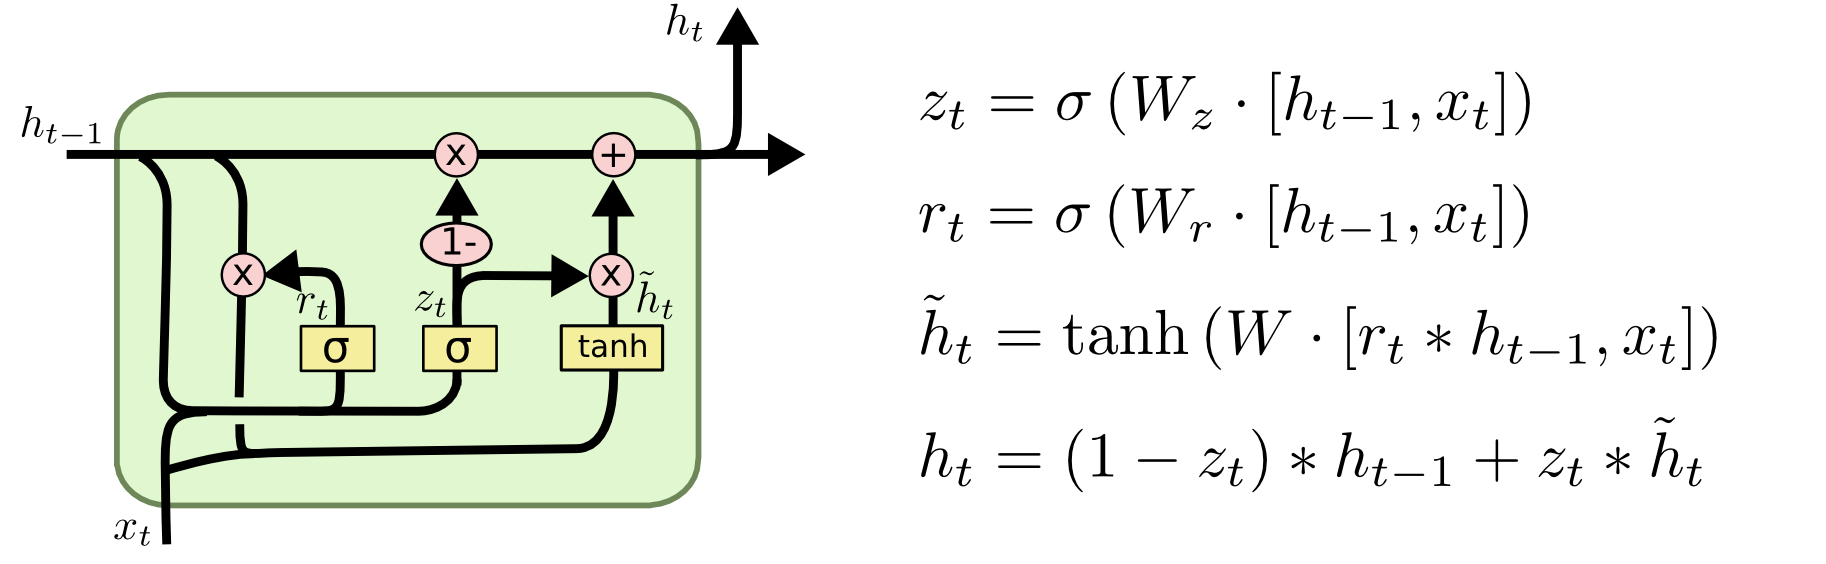
\includegraphics[scale=0.6]{./Figures/Ch_2_Background/GRU.png}
	}
	\caption{LSTM Gates and Configurations adapted from~\cite{colah}}
\end{figure}%

\subsubsection{BI-LSTM}\label{Sec:Bi_Lstm}

BI-LSTM refers to two LSTMs stacked on top of each other used to solve some problem where the information needs to be considered in both directions for LSTM. As the normal LSTM is working from left to right, the BI-LSTM adds the other directions into the learning information. Consider a motivation example regarding why we need BI-LSTM:

\begin{itemize}
\item \textit{Harry is the king, and he will travel next week.}
\item \textit{The new book which makes the big sale is named Harry Potter.}.
\end{itemize}

Harry in the first example refers to a person, but in the second example refers to a book. So, if we are working left to right, we do not get the type of word Harry represents in the second example.

The architecture in BI-LSTM is similar to what we discussed previously regarding Uni-LSTM. We can mention here that BI-LSTM is very slow compared to LSTM, and needs much time in the training phase but, as we see later in our research, it is impressive regarding the results and the effect on the language problems.

Figure~\ref{Fig:BI-LSTM} represents a recurrent neural network consisting of several LSTM blocks, processing the input sequence simultaneously forwards and backwards (to exploit both directions of temporal dependence). In Figure~\ref{Fig:LSTM_CharLevel} we can observe a similar example to our encoding data, which feeds the networks using a sequence of char, then passes to the BI-LSTM cells, then produces the character representations to feed the next layer of the network. Figure~\ref{Fig:LSTM_Arch} shows the simple example of the full network from char-level embedding (encoding) till the last sequence which outputs to softmax layer.%
\begin{figure}[!t]
 \centering
 \subfigure[bidirectional long short-term memory~\cite{Gitrepo_NN_Tikz}]
 {
  \label{Fig:BI-LSTM}
  \begin{tikzpicture}
	\node[rectangle] (Y0) at (0, 0) {$\dots$};
	\node[rectangle, draw, right=2em of Y0, minimum height=1cm, minimum width=1cm] (RNN) {LSTM$_\rightarrow$};
	\node[rectangle, right=of RNN, draw, minimum height=1cm, minimum width=1cm] (RNN2) {LSTM$_\rightarrow$};
	\node[rectangle, right=of RNN2, draw, minimum height=1cm, minimum width=1cm] (RNN3) {LSTM$_\rightarrow$};
			
	\node[rectangle, right= of RNN3, draw, minimum height=1cm, minimum width=1cm] (RNN4) {LSTM$_\rightarrow$};
	\node[rectangle, right=2em of RNN4] (RNN5) {$\dots$};
			
			
	\node[rectangle, above=of RNN4, draw, minimum height=1cm, minimum width=1cm] (R25) {LSTM$_\leftarrow$};
	\node[rectangle, left=of R25, minimum height=1cm, minimum width=1cm, draw] (R24) {LSTM$_\leftarrow$};
	\node[rectangle, left=of R24, draw, minimum height=1cm, minimum width=1cm] (R23) {LSTM$_\leftarrow$};
	\node[rectangle, left=of R23, draw, minimum height=1cm, minimum width=1cm] (R22) {LSTM$_\leftarrow$};
	\node[rectangle, left=2em of R22] (R21) {$\dots$};
	\node[right=2em of R25] (Y20) {$\dots$};
			
	\node[below=of RNN] (X1) {$\vec{x}_2$};
	\node[below=of RNN2] (X2) {$\vec{x}_3$};
	\node[below=of RNN3] (X3) {$\vec{x}_4$};
	\node[below=of RNN4] (X4) {$\vec{x}_5$};
	\node[above=of R25] (Y5) {$\vec{h}_5$};
	\node[above=of R24] (Y4) {$\vec{h}_4$};
	\node[above=of R23] (Y3) {$\vec{h}_3$};
	\node[above=of R22] (Y2) {$\vec{h}_2$};
			
	\draw[-stealth, thick] (X1) -- (RNN);
	\draw[-stealth, thick] (X2) -- (RNN2);
	\draw[-stealth, thick] (X3) -- (RNN3);
	\draw[-stealth, thick] (X4) -- (RNN4);
	\draw[-stealth, thick, densely dotted] (Y0) -- (RNN);
	\draw[-stealth, thick] (RNN) -- node[above, pos=0.35] {$\vec{h}_2^\rightarrow$} (RNN2);
	\draw[-stealth, thick] (RNN2) -- node[above, pos=0.35] {$\vec{h}_3^\rightarrow$} (RNN3);
	\draw[-stealth, thick] (RNN3) -- node[above, pos=0.35] {$\vec{h}_4^\rightarrow$} (RNN4);
	\draw[-stealth, densely dotted, thick] (RNN4) -- (RNN5);
	\node[below=4em of Y0] (d) {\dots};
	\node[below=4em of RNN5] (d) {\dots};
			
	\path[-stealth, ultra thick, white] (X1) edge[bend left=45] (R22);
	\path[-stealth, thick] (X1) edge[bend left=45] (R22);
	\path[-stealth, ultra thick, white] (X2) edge[bend left=45] (R23);
	\path[-stealth, thick] (X2) edge[bend left=45] (R23);
	\path[-stealth, ultra thick, white] (X3) edge[bend left=45] (R24);
	\path[-stealth, thick] (X3) edge[bend left=45] (R24);
	\path[-stealth, ultra thick, white] (X4) edge[bend left=45] (R25);
	\path[-stealth, thick] (X4) edge[bend left=45] (R25);
	\draw[-stealth, densely dotted, thick] (Y20) -- (R25);
			
	\draw[-stealth, thick] (R22) -- (Y2);
	\draw[-stealth, thick] (R23) -- (Y3);
	\draw[-stealth, thick] (R24) -- (Y4);
	\draw[-stealth, thick] (R25) -- (Y5);
		
	\draw[stealth-, densely dotted, thick] (R21) -- (R22);
	\draw[stealth-, thick] (R22) -- node[above, pos=0.65] {$\vec{h}_3^\leftarrow$} (R23);
	\draw[stealth-, thick] (R23) -- node[above, pos=0.65] {$\vec{h}_4^\leftarrow$} (R24);
	\draw[stealth-, thick] (R24) -- node[above, pos=0.65] {$\vec{h}_5^\leftarrow$} (R25);
	\draw[-stealth, densely dotted, thick] (Y20) -- (R25);	
			
	\path[-stealth, ultra thick, white] (RNN) edge[bend right=45] (Y2);
	\path[-stealth, thick] (RNN) edge[bend right=45] (Y2);
	\path[-stealth, ultra thick, white] (RNN2) edge[bend right=45] (Y3);
	\path[-stealth, thick] (RNN2) edge[bend right=45] (Y3);
	\path[-stealth, ultra thick, white] (RNN3) edge[bend right=45] (Y4);
	\path[-stealth, thick] (RNN3) edge[bend right=45] (Y4);
	\path[-stealth, ultra thick, white] (RNN4) edge[bend right=45] (Y5);
	\path[-stealth, thick] (RNN4) edge[bend right=45] (Y5);
			
\end{tikzpicture}

 }
 \subfigure[character-based representation using BiLSTM~\cite{ReimersG17}]
 {
 \label{Fig:LSTM_CharLevel}
  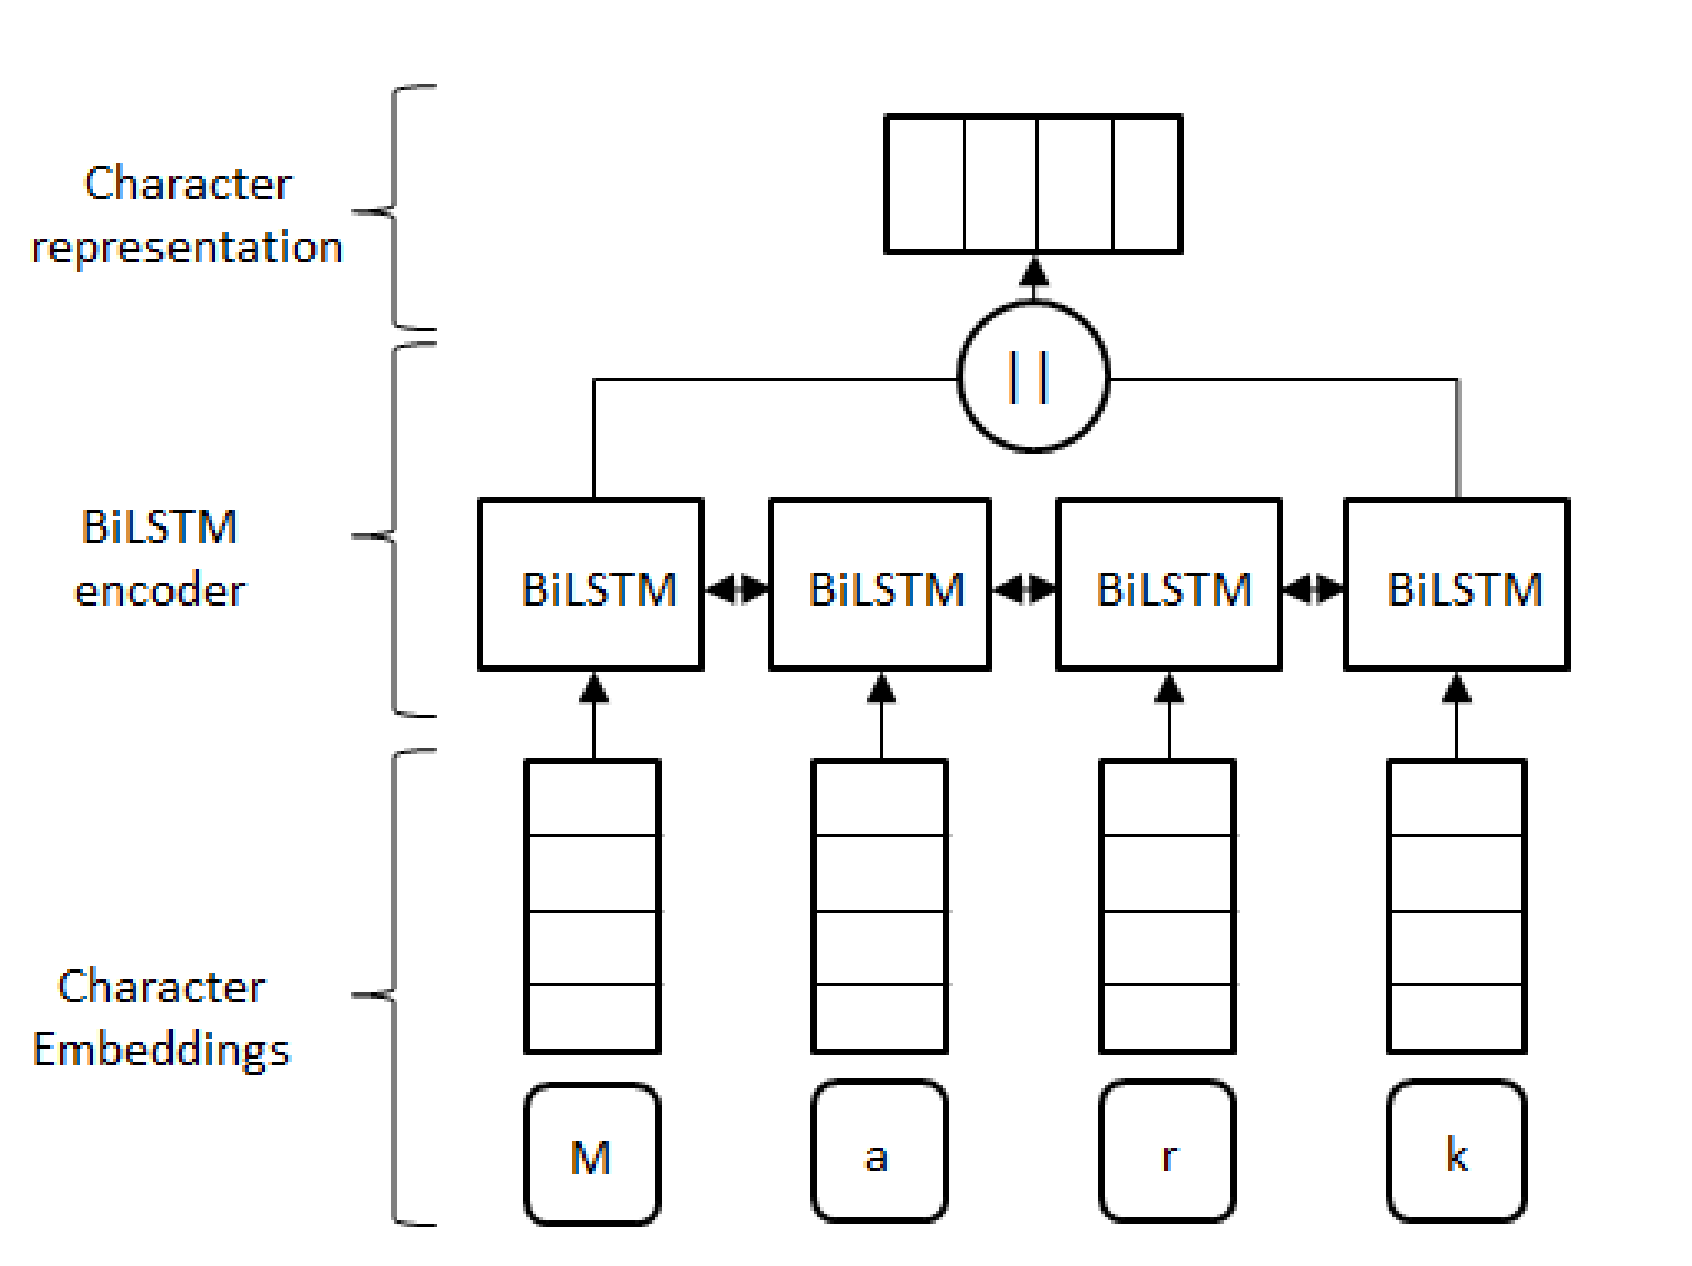
\includegraphics[width=8cm,height=7cm]{./Figures/Ch_2_Background/BI_LSTM_2.png}

 }
 \subfigure[An example of the architecture of LSTM~\cite{Blog_LSTM}]
 { 
  \label{Fig:LSTM_Arch}
  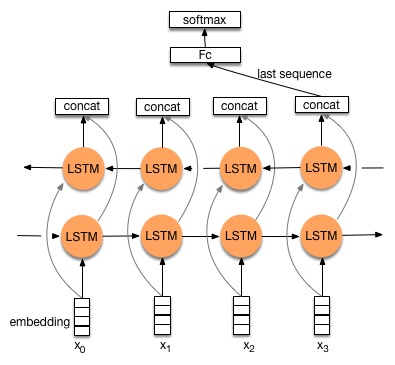
\includegraphics[width=8cm,height=7cm]{./Figures/Ch_2_Background/BI_LSTM_1.jpg}
 }
%\caption{LSTM Gates and Configurations adapopted from~\cite{colah}.}
\end{figure}%


\subsection{Machine Learning Model Assessment}

As explained previously, machine learning cycle starts by Data preparation, Feature extraction, Model training and Model assessment~\ref{Fig:Thesis_Cycle}. In this section we explain the meaning by model assessment. we also discuss different techniques for model assessment.

In Supervised machine learning problems, we have two types \textit{Classification and Regression}. Classification of the output is discrete variables, for example, Spam vs Normal Email detection. In Regression, the output is a continuous variable: for example, Predict Housing Price. Each type of problem has its methods or performance evaluation matrix. In this section, we focus on Classification problem, as our problem is a meter classifier application.

How can we measure the model performance? It is good when the difference between the predicted value and the actual is small and not overfitting on the development dataset.

There are many ways to measure classification performance. Before we explain every method, we give a simple example to allow us to understand the output of every method. Let us assume we have a binary classifier which detects Spam vs Normal Emails. we explain by example the definition for every type base on the example data in Table~\ref{Tab:EmailClassifier}%
\begin{table}[t]
 \centering
 \begin{tabular}{c c c c}
  \toprule
  \textbf{Label}& \textbf{Actual Number}& \textbf{Actual Spam (Positive)} & \textbf{Actual Normal (Negative)}\\
  \midrule
  Predicted as Spam (Positive)  & 200 & \cellcolor{green!25}160 & \cellcolor{red!25}40 \\
  Predicted as Normal (Negative)   & 300  & \cellcolor{red!25}10  & \cellcolor{green!25}290\\
  \bottomrule
 \end{tabular}
 \caption{Spam vs Normal Email Classifier example}\label{Tab:EmailClassifier}
\end{table}%
%
\subsubsection{Accuracy}

Accuracy measures the corrected prediction over the dataset. It is calculated using the ratio between the corrected predicted sample from the test data over the total test data sample. Ex: in Table~\ref{Tab:EmailClassifier}\textit{(the total positive predicted as positive + the total negative predicted as negative)/total number of test data}~\eqref{eq:accuracy_calculation} which means 90\%. An issue in Accuracy as a measurement is that it doesn’t give us any sense of the results with respect to the actual performance of the positive, calculated as positive and vice-versa. One measurement which gives us some sense is the Precision and Recall, which we discuss it in the next section.%
\begin{equation}\label{eq:accuracy_calculation}
\frac{\text{the total positive predicted as positive + the total negative predicted as negative}}{\text{total number of test data}} = \frac{160+290}{500}=0.9 
\end{equation}%


\subsubsection{Precision and Recall}

Precision and Recall are two measurements which answer questions related to our model performance. Some applications consider one of them and others require both or a combination. Before explaining it, we should prepare a data table named Confusion Matrix similar to the example in~\ref{Tab:EmailClassifier}.

\begin{itemize}
\item Precision (also called positive predictive value) is used to answer the question, \textbf{Based on the test data how many items predicted correctly from the test data sample}. It can be calculated from Equation~\eqref{eq:precision}.
\item Recall (also known as sensitivity) answers another question: \textbf{Based on the test data, how many of the truly predicted items are truly predicted}. We can calculate this using Equation~\eqref{eq:recall}.
\end{itemize}
\begin{equation}\label{eq:precision}
precision = \frac{\text{true positives}}{\text{true positives + false positives}} = \frac{160}{160 + 40}=0.8
\end{equation}%


\begin{equation}\label{eq:recall}
recall = \frac{\text{true positives}}{\text{true positives + false negatives}} = \frac{160}{160 + 10}=0.941
\end{equation}%

We need to highlight that some applications could require a focus on precision more than recall and vice-versa. We therefore need to choose the right measure based on our problem.
 
\subsubsection{$F_1$ Score}
In statistical analysis of binary classification, the F1 score is a measure of a test's accuracy. It considers both the precision \textit{p} and the recall \textit{r} of the test to compute the accuracy score. The F1 score is the harmonic average of the precision and recall, where an F1 score reaches its best value at 1 (perfect precision and recall) and worst at 0~\cite{Wiki_f1_score}. We can calculate it using Equation~\eqref{eq:f_1}.%
\begin{equation}\label{eq:f_1}
F_1= 2 \times \frac{precision*recall}{precision+recall}
\end{equation}%
 
\subsubsection{Per-Class Accuracy}

Per class, accuracy is one of the important accuracy measures when we have multi-class. There is a difference between each accuracy calculation regarding the dataset classes distribution. Most of the performance measurement calculate the average accuracy per-class but the difference is some of them take into consideration the size of each class and some don’t take the size. So, in case we have imbalanced dataset we should use the type which considers the class size for the accuracy of calculations. In case the data is imbalanced the results could hide information about how the model is performing. For example, assuming the model working perfectly with a class which has the most amount of our data and performing badly in the other class the accuracy can give us high results. However, if we use the average per-class, it will give us a more clear vision of how the model is performing regarding the dataset size for each class. Below is common types used in most of the framework to calculate accuracy per-class. Note: The below naming is followed the same as \textit{Sklearn} Library.

\begin{itemize}
 \item Weighted: Calculates the F1 score for each class independently but when it adds them together uses a weight that depends on the number of true labels of each class~\eqref{eq:f_1_weighted}.%
\begin{equation}\label{eq:f_1_weighted}
F_{1 class1}\times W_1 + F_{2 class2}\times W_2 + F_{3 class3}\times W_3
\end{equation}%

 \item Micro: Uses the global number of TP, FN, FP and calculates the F1 directly~\eqref{eq:f_1_micro}. It does not take into consideration the size for each class.%
 \begin{equation}\label{eq:f_1_micro}
F_{1 class1+class2+class3}
\end{equation}%
 \item Macro: Calculates the F1 separated by class but not using weights for the aggregation~\eqref{eq:f_1_macro}  which results in a bigger penalization when the model does not perform well with the minority classes.%
\begin{equation}\label{eq:f_1_macro}
F_{1 class1} + F_{2 class2} + F_{3 class3}
\end{equation}%
\end{itemize}

%%% Local Variables:
%%% mode: latex
%%% TeX-master: "../master"
%%% TeX-engine: xetex
%%% End:




%%% Local Variables:
%%% mode: latex
%%% TeX-master: "../master"
%%% TeX-engine: xetex
%%% End:


\newpage

\chapter{Literature Review}\label{Ch:Literature}
Poetry meter classification and detection have not addressed as a learning problem or similar our way for solving this problem. In this literature, we can see that they treat the problem mainly as deterministic. They are restricted by some static conditions and unable to build a scientific approach to address the problem.%

\section{Deterministic (Algorithmic) Approach}\label{sec:Determ_Algor_Appr}

~\cite{Abuata2016RuleBasedAlgorithm} present the work most related to our topic, classifying Arabic poetry according to its meters. However, they have not addressed it as a \textit{learning problem}; they have designed a \textit{deterministic five-step algorithm} for analyzing and detecting meters. The first and most important step is to have the input text carrying full diacritics; this means that every single letter must carry a diacritic, explicitly. The next step is converting input text into \textit{Arud writing} using \textit{if-else} like rules. \textit{Arud writing} is a pronounced version of writing; where only pronounced sounds written. Then metrical scansion rules are applied to the \textit{Arud writing}, which leaves the input text as a sequence of zeros and ones. After that, each group of zeros and ones is defined as a \textit{tafa'il}, giving a sequence of \textit{tafa'il}. Finally, the input text classifies the closest meter to the \textit{tafa'il} sequence. 82.2\% is the classification accuracy on a relatively small sample, of 417 verses.

\cite{Alnagdawi2013FindingArabicPoemMeter} has taken a similar approach to the previous work, but it replaced the \textit{if-else} by \textit{regular expressions} templates. This approach formalized the scansions, Arud based on lingual rules relating to pronounced and silent rules, directly related to \textit{harakat} as context-free grammar. Only 75\% of128 verses were correctly classified. 

\cite{Kurt2012AlgorithmForDetectionAnalysis} have taken a similar approach but worked on detecting and analyzing the arud meters in Ottoman Language. They convert the text into a lingual form in which the meters appear. Their first step is converting Ottoman text transliterated to Latin Transcription alphabet (LTA). Subsequently, they feed the text to the algorithm which uses a database containing all Ottoman meters to compare the detected meter extracted from LTA to the closest meter found in the database which saved the meters.

Both~\cite{Abuata2016RuleBasedAlgorithm} and~\cite{Alnagdawi2013FindingArabicPoemMeter} have common problems:

\begin{enumerate}
\item \textbf{The size of the test data} which cannot measure the accuracy for any algorithms they have constructed because it is a very small dataset. In addition, a 75\% total accuracy of 128 verses is even worse.
\item \textbf{The step converting verses into ones and zeros pattern} is probabilistic; it also depends on the meaning, which is a source of randomness. Treating such a problem as a deterministic problem will not satisfy the case study. It results in many limitations, including obligating verses to have full diacritics on every single letter before conducting the classification. This is also the case with~\cite{Kurt2012AlgorithmForDetectionAnalysis} work: for their algorithm to work, the text must be transliterated into LTA.
\end{enumerate}

We can summarize the results difference between our work and the previous work in Table~\ref{Tab:Summary_Results}

\begin{table}[h]
\centering
\begin{tabular}{c c c}
\toprule
\textbf{Ref.}& \textbf{Accuracy}& \textbf{Test Size} \\
\midrule
\cite{Alnagdawi2013FindingArabicPoemMeter} & 75\% & 128\\
\cite{Abuata2016RuleBasedAlgorithm}& 82.2\% & 417\\
This article & 96.38\%& 150,000 \\
\bottomrule
\end{tabular}
\caption{Overall accuracy of this article compared to literature.}\label{Tab:Summary_Results}
\end{table}


\section{English Literature}

\cite{Agirrezabal2016MachineLearningMetricalAnalysis} has used several machine learning models
(Naive Bayes, SVM, averaged perceptron, CRF, HMM) to automatically perform metrical scansion on
English poetry.  The models are trained on handcrafted-feature like number of syllables and others
which can be easily obtained by English NLP tools.

\cite{Tanasescu2016AutomaticClassificationOfPoetryMeterRhyme} This work is the ML
handcrafted-features version of ours, they classify poems by meter, they experimented different
classifier but the J48 design tree provided the most accurate results. Thanks to a program called
Scandroid and pronunciation dictionaries, they were able to extract the features that effect the
poetic pattern, features like the stresses position.

At this point, we have to notice that English poetry the Arabic poetry are two different patterns,
they deceptively share the same name which can lead to false hidden assumption like the techniques
done on English poetry can work on Arabic poetry, but what is true is non of the English techniques
can work on Arabic poems due to differences of the languages grammar and the pattern nature. English
pattern is much easier to be formalized for computers, which is not the case with Arabic.

\cite{Estes2016SupervisedMachineLearningForHybridMeter} develop a CRF model to predict the metrical
values of syllables in MHG epic verse. HandCraftedFeatures, Length of syllable in characters,
Syllable characters Syllable weight and length.



\cite{Hopkins2017AutomaticallyGeneratingRhythmic} has used generative models (LSTMs) to generate
rhythmic verses, what is special about this work is that they trained the models on both phonetic
character encoding. As usual in this kind of works on English poetry, they got the phonetics from a
dictionary (CMU pronunciation dictionary).  And found out that phonetic encoding is more informative
than character encoding.

\cite{Agirrezabal2017ComparisonFeatureBasedNeural} has extended his earlier feature-based models to
featureless neural network models. He showed that the character-based models are more informative
that the earlier feature-based models. He used Averaged Perceptron, Hidden Markov Models,
Conditional Random Fields (CRFs) and Bidirectional LSTMs with a CRF layer, the Bi-LSTM+CRF-model
outperformed them on scansion of poetry in two languages Spain and English.



%%% Local Variables:
%%% mode: latex
%%% TeX-master: "../master"
%%% TeX-engine: xetex
%%% End:

\newpage


\chapter{\uppercase{Dataset}}\label{ch:datasets}  

  The collection of the dataset was one of the most laborious tasks in this project. There were criteria we were searching to find. These criteria are as follows,
  \begin{itemize}
    
  \item \textbf{Datasets availability:} There are old Arabic references which have a lot of Poems but not all these books were not available in a PDF or a Web pages format, and it was hard to find it.
    
  \item \textbf{The Poem with diacritics:} There are resources which have Arabic Poems, but it is much harder to find same with diacritics.
    
  \item \textbf{The amount of the dataset:} To have a successful project with good results we need a massive amount of data. From the previous work, We did not find this amount of data. The maximum number found was 1.5k. However, We were searching for around 1.5M record of classified poetry.

  
\item \textbf{Cleansing of this data:} There was a limitation for the datasets which we can consider it, or we can scrap it due to the limitation for the APIs or the ready datasets in this context.
  
\end{itemize}
To meet the above criteria and overcome it, We applied following,

\begin{itemize}

  \item \textbf{Datasets availability:} We have scrapped the Arabic datasets from two big poetry websites: \textarabic{الديوان}~\cite{diwan}, \textarabic{الموسوعة الشعرية}~\cite{PoetryEncyclopedia2016}. Both merged into one large dataset, and we open sourced it online ~\cite{ArabicpoetryDS}.

  \item \textbf{The Poem with diacritics:} We tried to get the most verses with the available diacritics, but the diacritics states are not consistent, So, a verse can be fully diacritics, Semi diacritics or without diacritics.

\item \textbf{The amount of the dataset:} The total number of verses is 1,862,046 poetic verses; each verse labeled by its meter (class), the poet who wrote it, and the age which it was written. There are 22 meters, 3701 poets and 11 ages; and they are Pre Islamic, Islamic, Umayyad, Mamluk, Abbasid, Ayyubid, Ottoman, Andalusian, the era between Umayyad and Abbasid, Fatimid and modern. We are only interested in the 16 classic meters which attributed to Al-Farahidi, and they are the majority of the dataset with a total number of 1,722,321 verses. Figure~\ref{fig:data_size_distribution} shows the distribution of the verses per meter. %@@@ add datasets figures percentage per class
  
\item \textbf{Cleansing of this data:} Dataset was not cleaned enough for usage in this research, but we have applied cleansing rules explained in details in Data Preparation and Cleansing section~\ref{sec:data_clens}. We also open sourced all the code scripts used in our online repository~\cite{HCILAB_ArabicPoetry_2018}.
\end{itemize}

\begin{figure}
	\centering
	\begin{tikzpicture}[scale=1.2]
	\begin{axis}[
    symbolic x coords={Taweel,
   Kamel,
   Baseet,
   Khafeef,
   Wafeer,
   Rigz,
   Raml,
   Motakarib,
   Sar'e,
   Monsareh,
   Mogtath,
   Madeed,
   Hazg,
   Motadarik,
   Moktadib,
   Modar'e
    },
    xtick=data,
    % the following x label positioning does work here.
    every axis y label/.style= {at={( 0.15, 1.07)}, anchor=north},
    ylabel style={font=\footnotesize},
    xticklabel style = {font=\footnotesize},
    ylabel={Verses},
    height=8cm,
    x=0.4cm,
    x tick label style={rotate=90, anchor=east},
    enlarge y limits=0.07,
    name=left plot,%
    title=(a) \textit{Arabic Dataset},%
    title style={at={(0.5,-.4)}}%
  ]
    \addplot[ybar,color=black,mark=*, only marks,
	    point meta=explicit symbolic] coordinates {
        (Taweel, 416428)
        (Kamel,  370116)
        (Baseet, 244583)
        (Khafeef,     157880)
        (Wafeer,     143148)
        (Rigz,     119286)
        (Raml,     79560)
        (Motakarib,     63613)
        (Sar'e,     59370)
        (Monsareh,     28768)
        (Mogtath,     18062)
        (Madeed,     7808)
        (Hazg,     7468)
        (Motadarik,     5144)
        (Moktadib,     799 )
        (Modar'e,     288 )
    };

    \draw[loosely dotted] (axis cs:Taweel, 0) -- (axis cs:Taweel, 416428);
    \draw[loosely dotted] (axis cs:Kamel,  0) -- (axis cs:Kamel,  370116);
    \draw[loosely dotted] (axis cs:Baseet, 0) -- (axis cs:Baseet, 244583);
    \draw[loosely dotted] (axis cs:Khafeef,0) -- (axis cs:Khafeef,157880);
    \draw[loosely dotted] (axis cs:Wafeer, 0) -- (axis cs:Wafeer, 143148);
    \draw[loosely dotted] (axis cs:Rigz,   0) -- (axis cs:Rigz,   119286);
    \draw[loosely dotted] (axis cs:Raml,   0) -- (axis cs:Raml,   79560);
    \draw[loosely dotted] (axis cs:Motakarib, 0) -- (axis cs:Motakarib, 63613);
    \draw[loosely dotted] (axis cs:Sar'e, 0)   -- (axis cs:Sar'e, 59370);
    \draw[loosely dotted] (axis cs:Monsareh, 0) -- (axis cs:Monsareh,28768);
    \draw[loosely dotted] (axis cs:Mogtath, 0) -- (axis cs:Mogtath, 18062);
    \draw[loosely dotted] (axis cs:Madeed,  0) -- (axis cs:Madeed,  7808);
    \draw[loosely dotted] (axis cs:Hazg,    0) -- (axis cs:Hazg,    7468);
    \draw[loosely dotted] (axis cs:Motadarik,0) -- (axis cs:Motadarik, 5144);
    \draw[loosely dotted] (axis cs:Moktadib, 0) -- (axis cs:Moktadib,  799 );
    \draw[loosely dotted] (axis cs:Modar'e,  0) -- (axis cs:Modar'e,   288 );

\end{axis}



	\end{tikzpicture}%
	\caption{Arabic dataset Meter per class percentage ordered descendingly on x axis vs. corresponding meter name on y axis all class in the left of the red line (less than 1\% assume to be trimmed in some experiments).	}\label{fig:data_size_distribution}
\end{figure}

\section{Data Scraping}\label{sec:data_scrap}
To scrap the data from the website: \textarabic{الديوان}~\cite{diwan},ends up into such a problem just reduce your problem to the most smallest one. That means: First: Check if any "keywords" is set, if used. Then: Use your whole preamble and print the complete bibliography. If this ends up in the same error, your problem might be in your preamble. -> Reduction of preamble, until you get your bib printed. Adding slowly parts back to the preamble, until the error occurs again. That might show you, what lead to the warning.

 \textarabic{الموسوعة الشعرية}~\cite{PoetryEncyclopedia2016}, We used custom Python scripts for each websites to get the verses details. The script created with simple usage to pass the link we need to scrap. We will show two examples from both websites.
\begin{enumerate}
\item The First example, If we need to scrap a meter from \textarabic{الديوان} the website, for example Al-Tawil \\textit{https://www.aldiwan.net/poem.html?Word=\%C7\%E1\%D8\%E6\%ED\%E1\&Find=meaning}, We will pass this link to the script and the output file name. The script will start scraping and save the output in a CSV format. We can get the output similar than the output in table \ref{tables:Aldiwan_Sample}


% table: dal with diacritics
\begin{table}[H]
	\centering
	\begin{tabular}{c c c c c}
		%\hline
		\toprule
          \textbf{\small{\textarabic{البيت}}} & \small{\textbf{\textarabic{الشطر الأيسر}}} & \small{\textbf{\textarabic{الشطر الأيمن}}} &
\small{\textbf{\textarabic{البحر}}} & \small{\textbf{\textarabic{الشاعر}}} \\
		 %\hline
          \midrule
\makecell{\textarabic{رَجا شافع نسج المودّة بيننا}\\ \textarabic{ولا خيرَ في ودّ يكون بشافع}} &
\textarabic{ولا خيرَ في ودّ يكون بشافع} &                                                       \textarabic{رَجا شافع نسج المودّة بيننا} &                                                       \textarabic{الطويل}&
\textarabic{ابن نباته المصري}\\
          
		%\hline
		\bottomrule
	\end{tabular}
	\caption{Aldiwan scraping output example }\label{tables:Aldiwan_Sample}
\end{table}

\item Second Example, If we need to scrap the same meter from \textarabic{الموسوعة الشعرية} the website for example Al-Raml \textit{https://poetry.dctabudhabi.ae/\#/diwan/poem/126971}, We will pass this link to the script and the output file name. The script will start scraping and save the output in a CSV format. We can get the output similar than the output in table \ref{tables:ElMosoaa_Sample}


% table: dal with diacritics
\begin{table}[H]
	\centering
	\begin{tabular}{c c c c c c c c c}
		%\hline
          \toprule
\small{\textbf{\#}} &
\small{\textbf{\textarabic{البيت}}} &
\small{\textbf{\textarabic{الشطر الأيمن}}}&                        \small{\textbf{\textarabic{الشطر الأيسر}}} &
\small{\textbf{\textarabic{البحر}}}&                                 \small{\textbf{\textarabic{القافية}}}& \small{\textbf{\textarabic{الديوان}}}&                               \small{\textbf{\textarabic{الشاعر}}}&
\small{\textbf{\textarabic{العصر}}}\\
		 %\hline
          \midrule
1 &          
\makecell{\textarabic{من يرد مورد حب} \\ \textarabic{ظمأ بالشوق يزدد}} &
\textarabic{ظمأ بالشوق يزدد} &                                                        \textarabic{من يرد مورد حب} &                                                       \textarabic{الرمل}&
\textarabic{د}&
\makecell{\textarabic{الديوان} \\ \textarabic{الرئيسي}}&
\makecell{\textarabic{يعقوب الحاج}\\ \textarabic{ جعفر التبريزي}}&
\textarabic{الحديث}\\
          
		%\hline
		\bottomrule
	\end{tabular}
	\caption{Al-Mosoaa Elshearyaa scraping output example }\label{tables:ElMosoaa_Sample}
\end{table}
\end{enumerate}

We scrapped all the available datasets on both websites and merged them based on the common columns. Then we started the Data preparation tasks. We need to mention that, Not all diacritics was correctly available on all the websites. Also, We did not work to generate the diacritics for those datasets. So, we depended on whatever available without changing the data all the next sections is related to correction, preparation, and cleansing of the current datasets.
\newpage
\section{Data Preparation and Cleansing}\label{sec:data_clens}

Data preparation and cleansing tasks divided into multi-stages.
\begin{itemize}
\item Merge all scrapped datasets into one CSV file with a selection of the common columns in each file.
\item Remove the duplicates rows from the files in case we have any joined rows between both websites.
\item Filter the datasets on the 16 meters required as some data belonged to other non-famous or not original meters.
\item Remove many unnecessary white spaces which were useless.
\item Remove non-Arabic characters and the other web symbols.
\item Fix diacritics mistakes, such as the existence of two consecutive harakat, we have only kept one and have removed the other. %@@@add an example
\item Remove any \textit{harakah} comes after a white space, it removed as it is useless. %@@@add an example
\item We factored \textit{Shadaa}~\ref{def:shadaa_definition} to its original format explained in this example~\ref{tables:shadda_dal} previously.
\item We also factored \textit{Tanween}~\ref{def:tanween_definition} to its original format explained in this example~\ref{tables:Tanween_dal} previously.\footnote{\textit{We ignored the factorization of Alef-Mad  \textbf{\textarabic{ آ }} in our data preparation and transformation which can save more memory and shorten our encoding vectors}}
\end{itemize}

We need to highlight that the last two points are not a handcrafted feature. It is a factorization for the letter to its original format. This factorization will affect the size of the data in the memory and the letter representation in the vector. We will explain this part in details in the next chapter about encoding mechanism and the impact of the encoding type in the model training time and performance.







%%% Local Variables:
%%% mode: latex
%%% TeX-master: "../master"
%%% End:

\newpage

\chapter{\uppercase{Data Encoding}}\label{ch:data_encoding}

As we explained, We have collected the dataset and cleaned the data from any quality issues. The next step is to change the data representation to be ready for model training. This change of the data structure named \textit{Data Encoding}.

\section{Work embedding Encoding in English}\label{sec:word-level-english}
The concept of data encoding was first introduced by [Bengio et al., 2003]~\cite{Bengio2003}. They used an embedding lookup table as a reference and map every word to this lookup. They used the resulting dense vectors as input for language modeling. There are many works to improve the word embedding one of them [Collobert et al., 2011]~\cite{Collobert_2011} proposed improvement of word embedding task and proved the versatility of word embedding in many NLP tasks. Another work proposed by [Mikolov et al., 2013~\cite{Mikolov_2013};
Jeffrey Pennington et al., 2014~\cite{Pennington_2014} ] shows the maturity of word embedding and is currently the most used encoding technique in the neural network based natural language processing.

\section{Character Level Encoding in English}\label{sec:char-level-english}

All the previous work focused on word embedding encoding, but in our research problem here we do not work on word level we focus into character level encoding as input feature to the model. There is a good deal of research based on the character level encoding [Kim et al., 2015]~\cite{Kim_2015} used character level embedding to construct word level representations to work on out of vocabulary problem. [Chiu and Nichols, 2015]~\cite{Chiu_2015} also used character embeddings with a convolutional neural network for named entity recognition.[Lee, Jinhyuk et al.,2017]~\cite{ijcai_2017} used character embeddings for the personal name classification using Recurrent Neural Networks.

\section{Character Level Encoding in Arabic}\label{sec:char-level-arabic}

Working on Arabic language embedding based on the character level did not take much attention from the research community. [Potdar et al.,2017]~\cite{Potdar_2017} has done a comparative study on six encoding techniques. We are interested in the comparison of one-hot and binary. They have used Artificial Neural Network for evaluating cars based on seven ordered qualitative features. The accuracy of the model was the same in both encoding one-hot and binary. [Agirrezabal et al.,2017]\cite{Agirrezabal_2017} shows that representations of data learned from character-based neural models are more informative than the ones from hand-crafted features.

In this research, We will make a comparative study of different encoding techniques between binary and one-hot. Also, we provide some new encoding method specific for Arabic letters, and we will see the effect of this on our problem. We will show the efficiency of every technique based on performing model training and model running time performance.

Generally, a character will be represented as an n vector. Consequently, a verse would be an $n \times p$ matrix, where n
is the character representation length and p is the verse’s length, n varies from one encoding to another, we have used One-Hot and Binary encoding techniques and proposed a new encoding, the \textbf{Two-Hot} encoding.

Arabic letters have a feature related to the diacritics; To explain this feature we will take an example based on \textit{One-Hot} encoding. This feature is related to how we will treat the character with a diacritic. Arabic letters are 36 + white space as a letter. So, the total is 37. Any letter represented as a vector $37 \times 1$. Let's take an example a work such as \textarabic{مرحبا} having 5 letters encoded as a $37 \times 5$ matrix. If it came with diacritics such as \textarabic{مَرْحَبَا} and we need to represent the letters as One-Hot encoding we will consider every letter and diacritics as a separate letter. So, it will be 5 character and 4 diacritics. The vector shape will be $41 \times 9$.

One of the main reason we need to care about the encoding is the  \textit{RNN} training. If we have a different number of time steps in  \textit{RNN} cell and the input vector dimensions are different based on the input, It will have a standard architecture for the model and to be able to train both the work with diacritics and without diacritics to show the effect of the model learning on the same architecture.

To achieve the model architecture unification,  we proposed three different encoding systems: \textit{one-hot}, \textit{binary}, and the novel encoding system developed in this project \textit{two-hot}. The three of them explained in the next three subsections.

\begin{figure*}
  \centering
    \begin{tikzpicture}
    \node at (-12,0){\begin{tikzpicture}   
  % Rectangles
  % the space between each rectangular
  \def \x {0.57} 
  \def \s {1} % I'll use it to shift to right
  % A list of letters <3
  \newcommand\letters{{"ا","بَ","حَ", "رْ", "مَ"}}

  % Rectangle
  \def \length {2.95}
  \foreach \j in {0,...,4} 
  \draw [rounded corners=1pt] (\s+\x*\j, 0) rectangle (\s+0.5+\x*\j, \length) 
  node[above, xshift=-0.25cm]
  {\textarabic{\pgfmathparse{\letters[\j]}\pgfmathresult}};

  % Above Annotation
  % Cell line
  % 0.25*10+0.09 = 2.59
  \def \d {3.9 - 0.15}
  \draw (\s+0.25-0.007, 3.9 ) -- (\s+2.53+0.007, 3.9 ); % the main bar
  \draw (\s+0.25, 3.9 ) -- (\s+0.25, \d ); % sub bar #ا
  \draw (\s+0.25*3+0.03, 3.9 ) -- (\s+0.25*3+0.03, \d ); % sub bar #ب
  \draw (\s+0.25*5+0.15, 3.9+0.15 ) -- (\s+0.25*5+0.15, \d ) 
  node[above, yshift=0.3cm]{\textarabic{مَرْحَبَا}}; % sub bar #ح
  \draw (\s+0.25*7+0.2, 3.9 ) -- (\s+0.25*7+0.2, \d ); % sub bar #ر
  \draw (\s+2.53, 3.9 )  -- (\s+2.53, \d );  % sub-bar #م

  % adding numbers, vector ا
  \node at (\s+0.25, \length - 0.25)    {1}; % the top number; using -
  \node at (\s+0.25, \length - 0.6)     {0};
  \node at (\s+0.25, \length - 0.95)    {0};
  \node at (\s+0.25, \length - 1.3)     {0};
  \node at (\s+0.25,  1.1)     {\vdots};
  % \node at (\s+0.25, \length - 1.65)    {0};
  % \node at (\s+0.25, \length - 2)       {0};
  % \node at (\s+0.25, \length - 2.35)    {0};
  \node at (\s+0.25, \length - 2.7)     {0};

  % distance between vectors elements
  \def \d {0.07}
  % adding numbers, vector ب
  \node at (\s+0.25*3+\d, \length - 0.25)    {0}; % the top number; using -
  \node at (\s+0.25*3+\d, \length - 0.6)     {\vdots};
  % \node at (\s+0.25*3+\d, \length - 0.95)    {0};
  \node at (\s+0.25*3+\d, \length - 1.18)     {1};
  \node at (\s+0.25*3+\d, 1.28) {\vdots};
  \node at (\s+0.25*3+\d, \length - 2.35)    {0};
  \node at (\s+0.25*3+\d, 0.25) {0}; % The bottom  number


  % adding numbers, vector ح
  \node at (\s+0.25*5+\d*2, \length - 0.25)    {0}; % the top number; using -
  \node at (\s+0.25*5+\d*2, \length - 0.6)     {\vdots};
  \node at (\s+0.25*5+\d*2, \length - 1.35)     {1};
  \node at (\s+0.25*5+\d*2, 1.18) {\vdots};
  \node at (\s+0.25*5+\d*2, \length - 2.35)    {0};
  \node at (\s+0.25*5+\d*2, 0.25) {0}; % The bottom  number

  % adding numbers, vector ر
  \node at (\s+0.25*7+\d*3, \length - 0.25)    {0}; % the top number; using -
  \node at (\s+0.25*7+\d*3, \length - 0.6)     {0};
  \node at (\s+0.25*7+\d*3, \length - 0.95)     {0};
  \node at (\s+0.25*7+\d*3, \length - 1.33)     {\vdots};
  \node at (\s+0.25*7+\d*3, 1.07) {1};
  \node at (\s+0.25*7+\d*3, \length - 2.2)    {\vdots};
  \node at (\s+0.25*7+\d*3, 0.25) {0}; % The bottom  number

  % adding numbers, vector م
  \node at (\s+0.25*9+\d*4, 3 - 0.25) {0}; % the top number; using -
  \node at (\s+0.25*9+\d*4, 3 - 0.69) {0};
  \node at (\s+0.25*9+\d*4, 0.25) {0};
  \node at (\s+0.25*9+\d*4, 0.25*4 - 0.1) {\vdots};
  \node at (\s+0.25*9+\d*4, 0.9 + 0.4) {1};
  \node at (\s+0.25*9+\d*4, 1.3 + 0.6) {\vdots};

  % Vector size annotations.
  % figures starts at x = 1
  \def \d {0.6} % Annotation x=0.4
  \draw[arrows=->] (\d, 1.7) -- (\d, 2.9); % up-line
  \draw[arrows=<-] (\d, 0.1) -- (\d, 1.1) node[above, yshift=0.07cm]
  {\small{181}};
  % bottom-line

  % \draw[arrows=<-] (\s+0.1, -0.4) -- (\s+1.19, -0.4) node[right, xshift=0.05cm] {\small{5}};
  % \draw[arrows=->] (\s+1.2+0.5, -0.4) -- ( \s+2.7,-0.4);
\end{tikzpicture}%

%%% Local Variables:
%%% mode: latex
%%% TeX-master: "../main"
%%% End:

};
    \node at (-7,0){\begin{tikzpicture}[x=1cm,y=1cm]

  % Rectangles
  % the space between each rectangular
  \def \x {0.57} 
  \def \s {1} % I'll use it to shift to right
  % A list of letters <3
  \newcommand\letters{{"ا","بَ","حَ", "رْ", "مَ"}}

  % \draw[step=0.2, gray, very thin, red] (1,-0.5) grid (4,4);

  % Rectangulars
  \def \length {2.95}
  \foreach \j in {0,...,4} 
  \draw[rounded corners=1pt] (\s+\x*\j, 0) rectangle (\s+0.5+\x*\j, \length) 
  node[above, xshift=-0.25cm]
  {\textarabic{\pgfmathparse{\letters[\j]}\pgfmathresult}};

  % Above Annotatios
  % Cell line
  % 0.25*10+0.09 = 2.59
  \def \d {3.9 - 0.15}
  \def \z {0.2}
  \draw (\s+0.25-0.007, 3.9 ) -- (\s+2.53+0.007, 3.9 ); % the main bar
  \draw (\s+0.25, 3.9 ) -- (\s+0.25, \d ); % sub bar #ا
  \draw (\s+0.25*3+0.03, 3.9 ) -- (\s+0.25*3+0.03, \d ); % sub bar #ب
  \draw (\s+0.25*5+0.15, 3.9+0.15 ) -- (\s+0.25*5+0.15, \d ) 
  node[above, yshift=0.3cm]{\textarabic{مَرْحَبَا}}; % sub bar #ح
  \draw (\s+0.25*7+0.2, 3.9 ) -- (\s+0.25*7+0.2, \d ); % sub bar #ر
  \draw (\s+2.53, 3.9 )  -- (\s+2.53, \d );  % sub-bar #م

  % adding numbers, vector ا
  \node at (\s+0.25, \length - 0.25)    {0}; % the top number; using -
  \node at (\s+0.25, \length - 0.6)     {0};
  \node at (\s+0.25, \length - 0.95)    {0};
  \node at (\s+0.25, \length - 1.3)     {0};
  \node at (\s+0.25, \length - 1.65)    {0};
  \node at (\s+0.25, \length - 2)       {0};
  \node at (\s+0.25, \length - 2.35)    {0};
  \node at (\s+0.25, \length - 2.7)     {1};

  % distance between vectors elements
  \def \d {0.07}
  % adding numbers, vector ب
  \node at (\s+0.25*3+\d*1, \length - 0.25)    {0}; % the top number; using -
  \node at (\s+0.25*3+\d*1, \length - 0.6)     {0};
  \node at (\s+0.25*3+\d*1, \length - 0.95)    {1};
  \node at (\s+0.25*3+\d*1, \length - 1.3)     {0};
  \node at (\s+0.25*3+\d*1, \length - 1.65)    {0};
  \node at (\s+0.25*3+\d*1, \length - 2)       {1};
  \node at (\s+0.25*3+\d*1, \length - 2.35)    {1};
  \node at (\s+0.25*3+\d*1, \length - 2.7)     {1};


  % adding numbers, vector ح
  \node at (\s+0.25*5+\d*2, \length - 0.25)    {0}; % the top number; using -
  \node at (\s+0.25*5+\d*2, \length - 0.6)     {0};
  \node at (\s+0.25*5+\d*2, \length - 0.95)    {1};
  \node at (\s+0.25*5+\d*2, \length - 1.3)     {0};
  \node at (\s+0.25*5+\d*2, \length - 1.65)    {1};
  \node at (\s+0.25*5+\d*2, \length - 2)       {0};
  \node at (\s+0.25*5+\d*2, \length - 2.35)    {1};
  \node at (\s+0.25*5+\d*2, \length - 2.7)     {1};

  % adding numbers, vector ر
  \node at (\s+0.25*7+\d*3, \length - 0.25)    {1}; % the top number; using -
  \node at (\s+0.25*7+\d*3, \length - 0.6)     {0};
  \node at (\s+0.25*7+\d*3, \length - 0.95)    {0};
  \node at (\s+0.25*7+\d*3, \length - 1.3)     {1};
  \node at (\s+0.25*7+\d*3, \length - 1.65)    {1};
  \node at (\s+0.25*7+\d*3, \length - 2)       {0};
  \node at (\s+0.25*7+\d*3, \length - 2.35)    {1};
  \node at (\s+0.25*7+\d*3, \length - 2.7)     {1};

  % adding numbers, vector م
  \node at (\s+0.25*9+\d*4, \length - 0.25)    {0}; % the top number; using -
  \node at (\s+0.25*9+\d*4, \length - 0.6)     {0};
  \node at (\s+0.25*9+\d*4, \length - 0.95)    {1};
  \node at (\s+0.25*9+\d*4, \length - 1.3)     {1};
  \node at (\s+0.25*9+\d*4, \length - 1.65)    {1};
  \node at (\s+0.25*9+\d*4, \length - 2)       {1};
  \node at (\s+0.25*9+\d*4, \length - 2.35)    {0};
  \node at (\s+0.25*9+\d*4, \length - 2.7)     {1};

  % Vector size annotations.
  % figures starts at x = 1
  \def \vColumn {0.6} % Annotation x=0.4
  \draw[arrows=->] (\vColumn, 1.7) -- (\vColumn, 2.9); % up-line
  \draw[arrows=<-] (\vColumn, 0.1) -- (\vColumn, 1.1) node[above, yshift=0.07cm] {\small{8}};
  % bottom-line

  % \draw[arrows=<-] (\s+0.1, -0.4) -- (\s+1.19, -0.4) node[right, xshift=0.05cm] {\small{5}};
  % \draw[arrows=->] (\s+1.2+0.5, -0.4) -- ( \s+2.7,-0.4);

\end{tikzpicture}


%%% Local Variables:
%%% mode: latex
%%% TeX-master: "../main"
%%% End:

};
    \node at (0,0){% Defining a new box
\newsavebox{\columnVector}
% Populating the box
\savebox{\columnVector}{$\left[\begin{smallmatrix}k\\m\end{smallmatrix}\right]$}

\begin{tikzpicture}

  % The grid
  % \draw[step=0.5, gray!40, very thin] (0,0) grid (6,4);

  \def \recWidthA {0.5}
  \def \yStartA   {1.5}
  \def \yEndA     {3}
  \def \xStartA   {1.5}
  \def \xEndA     {0.5}
  \def \xStartB   {0}
  \def \yStartB   {1}
  \def \xEndB     {2}
  \def \yEndB     {3.5}
  \def \half      {\yEndA/2 - \yStartA/2}
  \def \xStartC   {3 +0.5}
  \def \yStartC   {0.5 -.1}
  \def \xEndC     {3.5 +0.5}
  \def \yEndC     {4 +.1 }
  \def \shiftMargin {0.3}
  \newcommand\numbers{{0.25, 0.6, 0.95, 1.3, 1.65, 2, 2.35, 2.7}}

  % Rectangle A
  \draw[rounded corners=2pt] (\xStartA, \yStartA) rectangle (\xStartA + \recWidthA, \yEndA)
  node [above, xshift=-.25cm] {\textarabic{◌َ}};
  % Populating the rectangle A
  \node at (0.25 + \xStartA, 3 -\numbers[0]) {1};
  \foreach \j in {1,...,3}
  \node at (0.25 + \xStartA, \yEndA -\numbers[\j]) {0};

  % Annotation A
  \node at (\xStartA-\shiftMargin, \yStartA + \half) {\small 4};
  \draw[arrows=-angle 90, very thin] (\xStartA-\shiftMargin, \yStartA + \half +.3) -- (\xStartA-\shiftMargin, \yEndA -0.1);
  \draw[arrows=angle 90-, very thin] (\xStartA-\shiftMargin, \yStartA + .1) -- (\xStartA-\shiftMargin, \yStartA + \half -.3);

  % Rectangle B
  \draw[rounded corners=2pt] (\xStartB +0.5, \yStartB) rectangle (\yStartB +0.5 -1.5, \yEndB)
  node[above, xshift=0.25cm] {\textarabic{ب}};
  \node at (\xStartB +0.25, \yEndB -\numbers[0]) {0};
  \node at (\xStartB +0.25, \yEndB -\numbers[1]) {1};
  \node at (\xStartB +0.25, \yEndB -\numbers[2]) {0};
  \node at (\xStartB +0.25, \yEndB -\numbers[3]) {0};
  \node at (\xStartB +0.25, \yEndB -\numbers[4] ) {\vdots};
  \node at (\xStartB +0.25, \yStartB +\numbers[0]) {0};

  % Annotation B
  \node at (-\shiftMargin, \yStartA + \half) {\small 37};
  \draw[arrows=-angle 90, very thin] (-\shiftMargin, \yStartA + \half +.3) -- (-\shiftMargin, \yEndB -0.1);
  \draw[arrows=angle 90-, very thin] (-\shiftMargin, \yStartB + .1) -- (-\shiftMargin, \yStartA + \half -.3);

  \node at (0.8, \yStartA +\half) {$+$};
  \node at (2.5 + .02, \yStartA +\half) {$=$};

  % Rectangle C
  \draw[rounded corners=2pt]  (\xStartC, \yStartC) rectangle (\xEndC, \yEndC)
  node[above, xshift=-0.25cm] {\textarabic{بَ}};
  ;
  \node at (\xStartC +0.25, \yEndC -\numbers[0]) {1};
  \node at (\xStartC +0.25, \yEndC -\numbers[1]) {0};
  \node at (\xStartC +0.25, \yEndC -\numbers[2]) {0};
  \node at (\xStartC +0.25, \yEndC -\numbers[3]) {0};

  \node at (\xStartC +0.25, \yEndC -\numbers[4] -.2) {0};
  \node at (\xStartC +0.25, \yEndC -\numbers[5] -.2) {1};
  \node at (\xStartC +0.25, \yEndC -\numbers[6] -.2) {0};
  \node at (\xStartC +0.25, \yEndC -\numbers[7] -.2) {\vdots};
  \node at (\xStartC +0.25, \yStartC +\numbers[0]) {0};

  % Annotation
  \node at (\xStartC -\shiftMargin, \yStartA +\half) {\small 41};
  \draw[arrows=-angle 90, very thin]  (\xStartC -\shiftMargin, 2.5) -- (\xStartC -\shiftMargin, \yEndC -0.1);
  \draw[arrows=angle 90-, very thin]  (\xStartC -\shiftMargin, 0.5) -- (\xStartC -\shiftMargin, 2);

  \draw [decorate,decoration={brace,amplitude=2pt,mirror,raise=2pt}, very thin]
  (\xEndC +\shiftMargin -.1, 2.5 +.2) -- (\xEndC +\shiftMargin  -.1, \yEndC -0.1);
%  node [right, midway, xshift=0.2cm, yshift=0.1cm] {\tiny $4 \times 1$ diacritic vector};

  \draw [decorate,decoration={brace,amplitude=2pt,mirror,raise=2pt}, very thin]
  (\xEndC +\shiftMargin -.1, 0.5) -- (\xEndC +\shiftMargin -.1, 2.4);
%  node [right, midway, xshift=0.2cm, yshift=0.1cm] {\tiny $37 \times 1$ letter vector};


  \node [rectangle, text width= 5em,font=\footnotesize] at (5.6, 3.4)
    {\scriptsize $4 \times 1$ letter vector which represents \textarabic{◌َ}};

  \node [rectangle, text width= 5em,font=\footnotesize] at (5.6, 1.4)
    {\scriptsize $37 \times 1$ letter vector which represents \textarabic{ب}};

  % \node at (0.25, 0.5) {$\bm m$};
  % \node at (1.5 +.25, 0.5 +0.5) {$\bm k$};
\end{tikzpicture}

%%% Local Variables:
%%% mode: latex
%%% TeX-master: "../main"
%%% End:

};
    \node at (-12+0.3,-3){(a) \textit{One-Hot}};
    \node at (-7+0.3, -3){(b) \textit{Binary}};
    \node at (0-0.5,  -3){(c) \textit{Two-Hot}};
\end{tikzpicture}


\caption{Different encoding mechanisms%: \textit{One-hot}, \textit{binary}, and \textit{two-hot}  encoding. Using the word example %\textarabic{مَرْحَبَا} \textit{One-hot} encoding is applied using $n$-letter alphabet $n = 181$ in Arabic. Same word encoded using \textit{binary} encoding where the vector length $n = \ceil*{\log_2 l}$, $l \in \{181\}$. \textit{two-hot} encoding is applied by stacking $\bm k_{4 \times 1}$ on the top of $\bm m_{37 \times 1}$ we get the $Two-Hot_{41 \times 1}$ \usebox{\columnVector}, which represents a letter and its diacritic simultaneously. 
}
\label{fig:One-Binary-Encoding}
\end{figure*}

\newpage
\subsection{One-Hot encoding}\label{sec:one-hot-encoding}
In this encoding system, We assume the letter with the diacritic as one unit. So, for example, \textarabic{د} represented as letter differs than (\textarabic{دَ, دِ, دُ, دْْ}). Now every letter is represented 5 times one without diacritic and four times with different diacritics combinations $36 \times 5$ besides the white-space character. So, the total is $181 \times 1$. From now forward, We have 181-characters Arabic alphabet represent the One-Hot encoding, and according to it, we will encode verses. (Figure~\ref{fig:One-Binary-Encoding}).

We need to mention that, One-Hot encoding technique is of the famous techniques in encoding problem. We will not compare the encoding technique in these sections. However, We will discuss it in details in model results. Also, The implementations of the One-Hot is trivial. But we need to focus on here about the size for every letter which is $181 \times 1$ which means if we have a verse with 82 characters it will results up with a matrix $181 \times 82$ which is very big to be in memory.

\subsection{Binary Encoding}\label{sec:binary-encoding}

The idea is to represent a letter with an $n \times 1$ vector which contains a unique combination of ones and zeros.  $n =\ceil*{\log_2} l$ where $l$ is the alphabet length, and $n$ is the sufficient number of digits to represent $l$ unique binary combinations.  For example a phrase like this \textarabic{مَرْحَبا}, it has 5 characters, figure~\ref{fig:One-Binary-Encoding} shows how it is encoded as a $8 \times 5$ matrix, which saves 22.6 times memory than the \textit{one-hot} and reduces the model input dimensions, significantly. But on the other hand, the input letter share some features between them due to the binary representation as it is shown in figure~\ref{fig:One-Binary-Encoding}.

\subsection{Two-Hot encoding}\label{sec:two-hot-encoding}
This is an intermediate technique which takes the advantages of the previous two encoding techniques. In which we encode the letter and its diacritic separately as two \textit{One-Hot} vectors, this way the letter is encoded as $37 \times 1$ \textit{One-Hot} vector and the diacritic is encoded as $4 \times 1$ \textit{One-Hot} vector, then both vectors stacked to form one $41 \times 1$ vector (Figure~\ref{fig:One-Binary-Encoding}).

By this way, we reduced the vector dimension from 181 to 41 and also minimizes the number of shared features between vectors to the maximum one at each vector. 



\newpage

\chapter{\uppercase{Model Training and Experiments}}\label{ch_model_training}

In this chapter, We will discuss the Training and Experiments done in this project. The training phase started by exploring what the ratio of Training, Testing, and Validation is. Choosing the correct percentage of training dataset compared to the Testing and Validation in Deep learning differs from normal machine learning structure, and it affects the model performance.

In a normal machine learning project, we used to split the dataset as around 60\% as training, 30\% testing and 10\% as a validation. However, In The Deep Learning, the amount of data profoundly affects the model performance. So, the more data fed as training, the more performance results the model can achieve on test data (Assuming we did the regularization and the needed generalization on the model training phase). Also, The main reason to change the split size is due to the size of the dataset we used to work on for example 1\% of 1M sample is 10k which is big enough for such experiments way. However, if we work on 10k sample, we need around 30\% 3k sample to have confidence in our model. So, it depends on the problem and size of the dataset.

In this research, We worked on \textit{Poem Comprehensive Dataset (PCD)}\cite{ArabicpoetryDS}. We are interested in the 16 classic meters which attributed to Al-Farahidi. These meters comprise the majority of the dataset with a total number of 1,722,321 verses. Figure ~\ref{fig:data_size_distribution} shows an ordered bar chart based on the number of verses per meter. We trained all our models based on 80\% which is around 1,377,856 verse. Our testing data(development) is 10\% around 172,232 verse, and our Validation data around 172,232 verse.

We can show training phase designed as a Data representation configurations and an RNN configuration. The number of experiments is the cross product of both data representation and RNN configuration, for example, If we have 12 data representation and 12 RNN configurations the total number of experiments will be 144. We need to highlight that,

\begin{itemize}
	\item Data representation feature is a general feature applied on the dataset not a Hand-Crafted features more details on ~\ref{sec_data_rep_param}.
	\item There is an effect of the Data representation feature due to Arabic language pronunciation and some features provide more information than others.
	\item RNN configurations are the parameters related to the Network model development training, and it used after many of experiment to find and tune the best configurations. These means we did more than the number of experiment written in this research but we only publish the best results overall. It will explain more details in sec ~\ref{sec_rnn_param}.
	\item The number verses used on testing and validation is a significant number 344,464 verse which confirms that the model tested on all types of verses and have confidence in the results.

\end{itemize}

\section{Parameters of Data Representation}\label{sec_data_rep_param}

Arabic language parameters have types Diacritics, Trimming, and Encoding. Every type has its effect on the data and the performance on model learning rate. We will explain each one in details in the next subsections.

\subsection{Diacritics}

Arabic dataset has the verse with diacritics. We can feed the network the characters with diacritics and without diacritics. With diacritics, it will be much easier for the network to learn since it provides more information on the pronunciation. Moreover, It provides more information related to the vowel and consonant sounds in the letters. However, as we discussed in Data Encoding Chapter~\ref{ch:data_encoding}, Both With and Without diacritics has the same length in input vector size.

\subsection{Trimming Small Classes}

Arabic poem dataset, as stated in Figure~\ref{fig:data_percentage_distribution}, is unbalanced. So, As part of our research, we make the dataset representation as a Full dataset and Trimmed dataset. This way allows us to study the effect of this unbalance. Also, We not only explore the impact of the unbalanced dataset But also, We have applied a technique to solve this issue~\ref{sec_rnn_param}. The trimmed classes are five classes which have less than 1\% of the total dataset. We presented this classes as all the classes on the left side of the horizontal red line in Figure~\ref{fig:data_percentage_distribution}. So, The total classes after trimming are 11 classes and the full with all 16 meters presented.

\subsection{Encoding Techniques}

As explained previously, There are three different encoding methods~\ref{ch:data_encoding}. Although all carry the same information, It expected that Every encoding has its behaviours as below,
\begin{itemize}
\item \textbf{Running Time}: It was expected the running time would differ from one encoding type compared to others. This information is important if someone has an experiment with limited time and need to get the results as fast as it can.
\item \textbf{Required Resources}: It was expected to have different resources consumption from one encoding typed compared to others. This information is important if someone has an experiment with limited resources.
• Learning Rate: Some encoding will learn faster than others (Note: Learning Rate not the overall performance) for example, one encoding can achieve 80\% on training performance after four epoch, but another one can reach the same percentage after 20\% epoch.
\item \textbf{Learning Rate}: The final performance percentage which can be achieved with every encoding technique (Note: the best can be the worst in learning rate or the method which take much time). So, the researcher who will use this encoding should decide which one will be used based on the criteria needed.

\item \textbf{Overall Performance}: The final performance percentage which can be achieved with every encoding technique (Note: the best can be the worst in learning rate or the method which take much time). So, the researcher who will use this encoding should decide which one will be used based on the criteria needed.

  \end{itemize}

  \subsection{Data Representation Matrix}

  The data representation matrix is the cross product of the Diacritics 2, Data Encoding 3, and Trimming 2 total 12 combinations table~\ref{table:data_representation_matrix} shows this matrix combination. Example (With diacritic + One-hot + Full)

  
\begin{table}[H]
  \centering
  \begin{tabular}{|c|c|c|c|c|c|}
    \hline
    \textbf{\#} & \textbf{Diacritic} & \multicolumn{3}{c|}{\textbf{Encoding Types}}  & \textbf{Trimming} \\
    
    \hline
    1 & With diacritic & One-hot & Two-hot & Binary & Full    \\
        \hline
    2 & Without diacritic & One-hot & Two-hot & Binary & Trimmed \\
\hline
 \end{tabular}
  \caption{Data Representation Combination Matrix}\label{table:data_representation_matrix}
\end{table}


\begin{figure}[H]
	\centering
	\begin{tikzpicture}
	
\begin{axis}
[
    axis lines*=left,
    title=Arabic Dataset Classes Percentage \%,
    xbar,
    width=17cm,
    height=14cm,
    xlabel={},
    symbolic y coords={Taweel, Kamel,Baseet,Khafeef,Wafeer,Rigz,Raml,Motakarib,Sar'e,Monsareh,Mogtath,Madeed,Hazg,Motadarik,Moktadib,Modar'e},
    ytick=data,
    xmin=0,
    xmax=.4, 
%    point meta={x*100},
    xtick={0.01,0.05,0.1,0.15,.2,.25,.3,.35},
    xticklabel={\pgfmathparse{\tick*100}\pgfmathprintnumber{\pgfmathresult}\%},
    point meta={x*100},
    nodes near coords={\pgfmathprintnumber\pgfplotspointmeta\%},
    nodes near coords align={horizontal},
    ]
  \addplot
[draw=blue,pattern=horizontal lines light blue] 
coordinates
     {
	(0.302,Taweel)
        (0.21489,Kamel)
        (0.1420,Baseet)
        (0.091,Khafeef)
        (0.083113,Wafeer)
        (0.069258866,Rigz)
        (0.04619348,Raml)
        (0.036934462,Motakarib)
        (0.034470926,Sar'e)
        (0.016703042,Monsareh)
        (0.010487011,Mogtath)
	(0.004533417,Madeed)
        (0.004336009,Hazg)
        (0.002986667,Motadarik)
        (0.000463909,Moktadib)
        (0.000167216,Modar'e)

};
  \draw [thick, dotted, draw=red] (10,-13) -- (10,500);
\end{axis}

	\end{tikzpicture}%
	\caption{Arabic dataset class size (number of verses) ordered descendingly on y-axis vs. corresponding meter name on the x-axis.}\label{fig:data_percentage_distribution}
\end{figure}

\newpage

\section{Parameters of Network Configuration}\label{sec_rnn_param}

% RNN,LSTM,BI_LSTM
As explained previously, Recurrent Neural Networks (RNN) showed the ability to solve language model problems in Section~\ref{sec_RNN}. We used RNNs with Long Short Term Memory(LSTM)~\ref{sec_LSTM} as the main architecture for our experiments. We also used BI-LSTM discussed in section~\ref{sec_bi-lstm} as an alternative way to test the affect of BI-Directional LSTM to check learn the patterns with the two directions.

We also thought using BI-LSTM will support the model to learn the Tafa'il for every class as it can combined the sound music from both ways. We will explain our argue and the effects on the results in Chapter~\ref{ch_results}.
% RNN Configuration
In RNNs network configuration parameters, there are four parameters:
\begin{itemize}
\item \textbf{Cell Type}: We used LSTM and BI-LSTM.
\item \textbf{Layers}: We tried many numbers of layers and we found the best number based on our problem is 4 and 7 layers.
\item \textbf{Cell Unit Size}: We also tried many numbers but the best results achieved from 50 and 82.
\item \textbf{Weighting Model}: As showed in Figure~\ref{fig:data_percentage_distribution} classes is unbalanced. So, as an alternative to remove the small classes we tried to keep all classes but with weighting the loss function to account for the relative class size. We introduced a new weighting function explain in next sub-section~\ref{sec_w_loss} to help working on all the dataset. So, we will have two combinations, One with weighting loss and one without weighting loss.
  
\end{itemize}

The total number of combination is 16 which is $4$ parameters each one have $2$ types. So, the total will be $2^4=16$; and hence, there are 16 different network configurations to run on each of the 12 data representations above. This results in $16 \times 12 = 192$ different experiments (or models). Hence, there are 96 different network configurations to run on each of the 2 data representations above. This results in 96 × 2 (= 192) different experiments (or models), whose accuracies are presented on the y-axis of Figure 7-a.%@@@add figure
For all the 192 experiments networks are trained using dropout of 0.2, batch size is of 2048, with Adam optimizer, and 10\% for each of validation and testing sets.

\textit{Experiments are conducted on a Dell Precision T7600 Workstation with: Intel Xeon E5-2650 32x 2.8GHz CPU, 32GB RAM, 1 NVIDIA GeForce GTX 1080 ti GPU, Hard desk SSD 256; and with: Ubuntu OS, x86\_64 Linux 16.04 LTS.}

\newpage
\subsection{Working on Unbalanced data using Weighted Loss}\label{sec_w_loss}

One of the important problem we worked to solve it during our research unbalance dataset issue. We worked to overcome the unbalanced dataset and to not make our model suffer from this issue. We so introduced a Weighting function~\ref{eq:training_weighted_fun} where nc is the sample size of class c, c = 1,2,...C, and C
is the total number of classes.

\begin{align}
  w_c &= \left(\frac{\frac{1}{n_c}}{\sum_c \frac{1}{n_c}} \right),\label{eq:training_weighted_fun}
\end{align}

The idea is to increase the loss for the small classes as the number of verses of small classes is small so the output will be bigger than the loss in case the class has a lot of verses. To have a clear explanation we can show equation~\ref{eq:training_weighted_fun_example} as example the biggest class will has smaller loss compared to the smallest class. We are dividing on constant which is the sum of classes density

\begin{subequations}
\begin{align}
  w_c &=  \frac{\frac{1}{288}}{\sum\frac{1}{416428}+\frac{1}{370116}\dots+\frac{1}{288}}\\
      &= \frac{\frac{1}{288}}{0.00534631950086646} = ~0.0312768 \\
        &= \frac{\frac{1}{416428}}{0.00534631950086646} = ~0.0004491642
\end{align}\label{eq:training_weighted_fun_example}
\end{subequations}

%@@@@@@ some details about the training and tools used 
\newpage


\chapter{\uppercase{Results And Discussion}}\label{ch:Results}

In this chapter we will explain the results of all the 192 experiments on our dataset. We measure the results using the overall $F_1$ Score Then we measure the performance accuracy of the model per class (meter).We will start by present the results for every combinations and then discuss our findings related to the topic.

\section{Results}

As we explained, In Chapter~\ref{ch:Model_Training} we have a set of combinations we need to explore it. So, most of our results will combine a combination and show the results of this combinations. Let's explore it as below,
\begin{enumerate}
\item  We have three data representation \textbf{\textit{Binary, One-hot, and Two-Hot}} we will represent it as \textbf{\textit{BinE, 1D, 0T}} respectively.
\item We have two types of model loss functions \textbf{\textit{Weighting loss and no Weighting loss}} we will represent it as \textbf{\textit{(1 and 0)}} respectively.
\item Number of layers is represented as \textbf{\textit{nL}} for example, 7 layers is 7L.
  \item Number of cell units is represented as \textbf{\textit{nU}} for example, 82 unit is 82U.
  \end{enumerate}

  So, If we need to explain a set of combination we can write (4L, 82U, 0) which means 4 layers, 82 units, and no weighted loss function. Also, we will provide many figures every figure will explain specific result perspective.
  
\subsection{Overall F1 Score}

\textbf{$F_1$ (also F-score or F-measure)} is a measure of a test's accuracy. It considers both the precision $p$ and the recall $r$ of the test to compute the score: $p$ is the number of correct positive results divided by the number of all positive results returned by the classifier, and $r$ is the number of correct positive results divided by the number of all relevant samples (all samples that should have been identified as positive).\\ The F1 score is the harmonic average of the precision and recall, where an F1 score reaches its best value at 1 (perfect precision and recall) and worst at 0~\cite{Wiki_f1_score}.


We present the $F_!$ Score in Figure~\ref{fig:ArabicModelsResults} of the 16 neural netwroks configurations and at each of the 12 data representations (y- and
x-axis respectively). The x-axis is divided into 4 strips corresponding to the 4 combinations of trimming and diacritic parameters. Then, each strip includes the 3 different encoding values. Each point on the figure represents the F1 score of one of the 192 experiments; (some values are too small, and hence omitted from the figure). To explain the figure, we take as an example the most-left
vertical list of points that represents the 16 experiments of the full (no trimming), diacritics, and binary encoding dataset representation.

The best network out of the 16 configurations is listed at the top: 7 layers, size of 82, and no loss weighting (7L, 82U, 0W). This network possess 90.25 F1 score by the Bi-LSTM cell (indicated by the large circle).

The best LSTM model is indicated by the square point, and possess 79.77 F1 score. Among all the 192 experiments, the highest F1 score is 96.38 and is possessed by a network configuration of (4L, 82U, 0) on (1T, 0D, BinE).

\subsubsection{Data Representation Effects}

In this section we will explain the effect of the 12 data representation technique we explained it previous.

\begin{enumerate}
\item \textbf{Trimming Effect:} The effect of trimming( remove the small classes from training cycle) can be observed if we fix the other two parameters, diacritic and encoding. The score with trimming is consistently higher than that with no trimming. E.g., by looking at the two unshaded strips, the score at (1T, 0D, TwoE) is 0.9629, while that at (0T, 0D, TwoE) is 0.9411. The only exception, with a very little difference, is (1T, 1D, BinE) vs. (0T, 1D, BinE). We need highlight that is logic to have this effect as the training will have less classes with huge amount of data for these classes.
\item \textbf{Diacritics Effect}
  \begin{itemize}
  \item \textit{Without Trimming:} The effect of diacritics is obvious only with no trimming (the two left strips of the figure), where, for each encoding, the F1 score is higher for diacritics than no diacritics.
    \item \textit{With Trimming:} The diacritics doesn't have except for the \textit{one-hot} encoding but other encoding doesn't have an effect on the model performance. This result is inconsistent with what is anticipated from the effect of diacritics. We think that this result is an artifact due to the small number of network configurations.

    \end{itemize} 
\item \textbf{Encoding Effect:} The effect of encoding is clear; by looking at each individual strip, \textit{$F_1$ score is consistently highest for two-hot then one-hot then binary—the} only exception is (1T, 0D, BinE) that performs better than the other two encodings. It seems that two-hot encoding makes it easier for networks to capture the patterns in data. However; we anticipate that there is a particular network architecture for each encoding that is capable of capturing the same pattern with yielding the same score.

  
  \end{enumerate}


  
\begin{figure}[!t]
 \begin{tikzpicture}
  %% Uses pointModelsFiguresStyle macro defined in pgfplot_configurations.tex

  %% two grid to help during positioing.
  % \draw[step=0.2, green!40, thin] (0,0) grid (8,6);
  % \draw[step=1, red!40, very thin] (0,-1) grid (8,7);

  %% Variables
  \def \maxHeight{5.7}
  \def \yONE{-0.8}
  \def \yTWO{-0.3}

  %% two colored areas to distinguish the diacritics models.
  \fill[gray!30, opacity=0.2, rounded corners=2pt] (0,-0.5) rectangle (2.1,\maxHeight);
  \fill[gray!30, opacity=0.2, rounded corners=2pt] (4.2,-0.5) rectangle (6.32,\maxHeight);

  %% The Full/Elimenated Seperator
  \draw[dashed, thick] (4.2, 0 - 0.9) -- (4.2, \maxHeight +0.5);

  %% Group Labels Full/Elimenated
  \node [align=center, text width=3cm, inner sep=0.25cm] at (2.1, \yONE) {\scriptsize No Trimming(0T)};
  \node [align=center, text width=4cm, inner sep=0.25cm] at (6.32,\yONE) {\scriptsize Trimming(1T)};

  \node [align=center, text width=3cm, inner sep=0.25cm] at (1, \yTWO) {\scriptsize Diacritics(1D)};
  \node [align=center, text width=3cm, inner sep=0.25cm] at (3, \yTWO) {\scriptsize No Diacritics(0D)};
  \node [align=center, text width=3cm, inner sep=0.25cm] at (5+0.2, \yTWO) {\scriptsize Diacritics(1D)};
  \node [align=center, text width=3cm, inner sep=0.25cm] at (7+0.2, \yTWO) {\scriptsize No Diacritics(0D)};

  % Points annotaions
  \def \layerHeight{5.7}
  \def \unitHeight{\layerHeight - 0.3}
  \def \weightedHeihgt{\layerHeight - 0.6}

  \def \step{0.2}

  %%%%%% 

  \node  at (3.5*   \step -0.15, \layerHeight) {\scriptsize 7L};
  \node  at (3.5*   \step -0.15, \unitHeight) {\scriptsize 82U};
  \node  at (3.5*   \step -0.1, \weightedHeihgt) {\scriptsize 0};

  \node  at (5.2*   \step, \layerHeight) {\scriptsize 7L};
  \node  at (5.2*   \step, \unitHeight) {\scriptsize 50U};
  \node  at (5.2*   \step, \weightedHeihgt) {\scriptsize 1};

  \node  at (7*     \step +0.15, \layerHeight) {\scriptsize 7L};
  \node  at (7*   \step   +0.15, \unitHeight) {\scriptsize 50U};
  \node  at (7*   \step   +0.1, \weightedHeihgt) {\scriptsize 1};

  %%%%%%

  \node  at (14*    \step -0.15, \layerHeight) {\scriptsize 7L};
  \node  at (14*   \step -0.15, \unitHeight) {\scriptsize 82U};
  \node  at (14*   \step -0.1, \weightedHeihgt) {\scriptsize 0};

  \node  at (16*    \step, \layerHeight) {\scriptsize 7L};
  \node  at (16*    \step, \unitHeight) {\scriptsize 82U};
  \node  at (16*    \step, \weightedHeihgt) {\scriptsize 0};

  \node  at (17.6*  \step +0.15, \layerHeight) {\scriptsize 7L};
  \node  at (17.6*  \step +0.15, \unitHeight) {\scriptsize 50U};
  \node  at (17.6*  \step +0.1, \weightedHeihgt) {\scriptsize 0};

  %%%%%%

  \node  at (24.5*  \step -0.15, \layerHeight) {\scriptsize 7L};
  \node  at (24.5*  \step -0.15, \unitHeight) {\scriptsize 82U};
  \node  at (24.5*  \step -0.1,  \weightedHeihgt) {\scriptsize 1};

  \node  at (26.1*  \step, \layerHeight) {\scriptsize 7L};
  \node  at (26.1*  \step, \unitHeight) {\scriptsize 82U};
  \node  at (26.1*  \step, \weightedHeihgt) {\scriptsize 0};

  \node  at (28*    \step +0.15, \layerHeight) {\scriptsize 7L};
  \node  at (28*    \step +0.15, \unitHeight) {\scriptsize 82U};
  \node  at (28*    \step +0.1,  \weightedHeihgt) {\scriptsize 1};

  %%%%%%

  \node  at (35*    \step -0.15, \layerHeight) {\scriptsize 4L};
  \node  at (35*    \step -0.15, \unitHeight) {\scriptsize 82U};
  \node  at (35*    \step -0.1,  \weightedHeihgt) {\scriptsize 0};

  \node  at (37*    \step, \layerHeight) {\scriptsize 7L};
  \node  at (37*    \step, \unitHeight) {\scriptsize 50U};
  \node  at (37*    \step, \weightedHeihgt) {\scriptsize 0};

  \node  at (38.7*  \step +0.15, \layerHeight) {\scriptsize 4L};
  \node  at (38.7*  \step +0.15, \unitHeight) {\scriptsize 50U};
  \node  at (38.7*  \step +0.1,  \weightedHeihgt) {\scriptsize 1};

  \begin{axis}[
    major x tick style = transparent,
    ybar=2*\pgflinewidth,
    x=10pt,
    ymajorgrids = true,
    % every axis y label/.style= {at={( 0, 1.09)}, anchor=north},
    ylabel = {$F_1$ Score},
    ylabel style = {font=\footnotesize},
    xtickmin={1},
    xtickmax={21},
    axis x line = bottom,
    axis y line = left,
    enlarge y limits={upper, value=0.1},
    xticklabels = {,,},
    bar shift=0pt,
    % scaled y ticks = false,
    enlarge x limits=0.1,
    ymin=0.76,
    ymax=0.98,
    legend style={at={(0.5, -0.2)}, anchor=north, legend columns=3},
    % legend style={at={(0.9, 0.26)}, anchor=north, legend columns=1},
    every axis legend/.append style={nodes={right}},
    nodes near coords={\vspace*{0.1\baselineskip}
      \foreach \X in \pgfplotspointmeta%
      {\centerline{\X}\newline}%
      \vspace*{-0.7\baselineskip}
    },
    nodes near coords style={font=\scriptsize,anchor=-90, text width=1cm},
    ]

    % Settings:
    % x-axis values are 1,2,3,..,21

    % Full takes 1,..,10
    % Full-with-diacritics takes 1,2,3
    % Full-without-diacritics takes 7,8,9

    % (14,21
    % (14, 15
    % (14, 21

    % Separators 5, 11, 17

    %%%%%%%%%%%%%%%
    %% Full Dataset
    %%%%%%%%%%%%%%%
    % Binary
    \addplot[pointBiLSTM=blue] coordinates {
      (1, 0.9025) %[7L~~,82U~~~,0] % Full,Diacritics,Binary
      (7, 0.8767)  %[7L~~~,82U~~~,0] % Full,Without-Diacritics,Binary

    };
    % OneHot
    \addplot[pointBiLSTM=red] coordinates {
      (2, 0.9347) %[7L,50U,1] % Full,Diacritics,OneHot
      (8, 0.9310) %[7L,82U,0] % Full,Without-Diacritics,OneHot
    };
    % TwoHot
    \addplot[pointBiLSTM=brown] coordinates {
      (3, 0.9485) %[~7L,~~~50U,1] % Full,Diacritics,TwoHot
      (9, 0.9411) %[7L,50U,0] % Full,Without-Diacritics,TwoHot
    };
    %%%%%%%%%%%%%%%%%%%%%
    %% Trimmed Dataset
    %%%%%%%%%%%%%%%%%%%%%
    % Binary
    \addplot[pointBiLSTM=blue] coordinates {
      (13, 0.8989)  %[7L~~,82U~~~,1]  % (14,Binary
      (19, 0.9638)  %[4L,82U,0]  % (14,Binary
    };
    % OneHot
    \addplot[pointBiLSTM=red] coordinates {
      (14, 0.9473) %[7L~~,82U~~~,0] % (14,OneHot
      (20, 0.9435) %[7L,50U,0] % (14,OneHot
    };
    % TwoHot
    \addplot[pointBiLSTM=brown] coordinates {
      (15, 0.9547) %[~7L,~~~82U,1] % (14,TwoHot
      (21, 0.9629) %[3L,50U,1] % (14,TwoHot
    };
    %%%%%%%%%%%%%%%%%%%%%
    %% LSTM models [squares]
    %%%%%%%%%%%%%%%%%%%%%
    % Binary
    \addplot[pointLSTM=blue] coordinates {
      (1,  0.7977761225792722)
      (7,  0.7883237568276938)
      (13, 0.827841810615813)
      (19, 0.8163877496033292)
    };
    % OneHot
    \addplot[pointLSTM=red] coordinates {
      (2,  0.8965678276701898)
      (8,  0.8869854106074577)
      (14, 0.9094811843247612)
      (20, 0.926671257072718)
    };
    % TwoHowt
    \addplot[pointLSTM=brown] coordinates {
      (3,  0.9170331749071908)
      (9,  0.8972239956491925)
      (15, 0.94120887345448)
      (21, 0.9284854653773612)
    };
    %%%%%%%%%%%%%%%%%%%%%
    %% The rest models
    %%%%%%%%%%%%%%%%%%%%%
    % Binary
    \addplot[pointRug=blue, mark size=0.7pt]
    coordinates {
      % 1, 7, 13, 19
      (19, 0.8182558452833577)
      (19, 0.9638475586025208)
      (19, 0.9619555129778764)
      (19, 0.9611891147501721)
      (19, 0.6499715594407688)
      (19, 0.9576864353501182)
      (19, 0.7611831272640182)
      (19, 0.6869083615244139)
      (19, 0.7495314792084543)
      (19, 0.6293147322096818)
      (19, 0.704074484327755 )
      (19, 0.9556686525162408)
      (19, 0.9604047540640064)
      (19, 0.9621052001317248)
      (19, 0.7838038499535971)

      (13, 0.8986558093584407)
      (13, 0.8988593838876747)
      (13, 0.8555698589947011)
      (13, 0.8649043499086908)
      (13, 0.8203873903541598)
      (13, 0.7581235218393557)
      (13, 0.8634134658563603)
      (13, 0.6457563691883963)
      (13, 0.7879471903721222)
      (13, 0.7406280872975481)
      (13, 0.8841181929766787)
      (13, 0.8741370535580636)
      (13, 0.770906804778014 )
      (13, 0.8288896206927522)
      (13, 0.8079693440708918)

      (7, 0.2392116525974793)
      (7, 0.7722328627840438)
      (7, 0.817325199214963 )
      (7, 0.8267420964271358)
      (7, 0.8307795984961339)
      (7, 0.2392116525974793)
      (7, 0.7268331323449433)
      (7, 0.7918174079591402)
      (7, 0.8564115296398761)
      (7, 0.7346362110141638)
      (7, 0.2392116525974793)
      (7, 0.7977524768863352)
      (7, 0.8766640656404436)
      (7, 0.5082878153744296)
      (7, 0.7272055520087016)

      (1, 0.8614953536213379)
      (1, 0.8794601688302476)
      (1, 0.2392116525974793)
      (1, 0.2392116525974793)
      (1, 0.8706225910950319)
      (1, 0.8677259937102457)
      (1, 0.6374642358894327)
      (1, 0.5386134165661725)
      (1, 0.2392116525974793)
      (1, 0.2392116525974793)
      (1, 0.8948003121231468)
      (1, 0.6666016410110899)
      (1, 0.866862925918044 )
      (1, 0.9025442765600246)
      (1, 0.8869558534912866)
    };

    % OneHot
    \addplot[pointRug=red, mark size=0.7pt]
    coordinates {
      % 2, 8, 14, 20

      (20, 0.9234859144388228 )
      (20, 0.24334939975451306)
      (20, 0.24334939975451306)
      (20, 0.24334939975451306)
      (20, 0.9015956650600244 )
      (20, 0.24334939975451306)
      (20, 0.24334939975451306)
      (20, 0.24334939975451306)
      (20, 0.9361973475436338 )
      (20, 0.9426518576175792 )
      (20, 0.9435140556237464 )
      (20, 0.24334939975451306)
      (20, 0.9382570427805884 )
      (20, 0.9427656198545042 )
      (20, 0.9328263928389664 )

      (14, 0.9334371164266684 )
      (14, 0.24334939975451306)
      (14, 0.93929287788522   )
      (14, 0.9401011885160016 )
      (14, 0.940059276112924  )
      (14, 0.24334939975451306)
      (14, 0.24334939975451306)
      (14, 0.24334939975451306)
      (14, 0.24431937251145106)
      (14, 0.93308984222974   )
      (14, 0.9352632997036194 )
      (14, 0.8778253450288896 )
      (14, 0.24334939975451306)
      (14, 0.24334939975451306)
      (14, 0.9472562344699575 )


      (8, 0.9298964318649358)
      (8, 0.2392116525974793)
      (8, 0.9212184625570452)
      (8, 0.2392116525974793)
      (8, 0.2392116525974793)
      (8, 0.2392116525974793)
      (8, 0.2392116525974793)
      (8, 0.2392116525974793)
      (8, 0.2392116525974793)
      (8, 0.2392116525974793)
      (8, 0.2392116525974793)
      (8, 0.9026743278711784)
      (8, 0.9146094913811448)
      (8, 0.9298964318649358)
      (8, 0.9310432479723818)
      (8, 0.9275673311106382)

      (2, 0.2392116525974793)
      (2, 0.9346846846846848)
      (2, 0.9320954813080796)
      (2, 0.922241138776572 )
      (2, 0.8536213378733064)
      (2, 0.2392116525974793)
      (2, 0.9248953678087536)
      (2, 0.2392116525974793)
      (2, 0.2392116525974793)
      (2, 0.2392116525974793)
      (2, 0.2392116525974793)
      (2, 0.9309841337400392)
      (2, 0.2392116525974793)
      (2, 0.9336324513489868)
      (2, 0.2392116525974793)
    };
    % TwoHot
    \addplot[pointRug=brown, mark size=0.7pt]
    coordinates {
      % 3, 9, 15, 21

      (21, 0.9100978953986169 )
      (21, 0.24334939975451306)
      (21, 0.24334939975451306)
      (21, 0.24334939975451306)
      (21, 0.9445379157560698 )
      (21, 0.9396281771098404 )
      (21, 0.9380534682513548 )
      (21, 0.24334939975451306)
      (21, 0.9627219112055804 )
      (21, 0.9628835733317368 )
      (21, 0.9255635721342396 )
      (21, 0.9427356824237344 )
      (21, 0.24334939975451306)
      (21, 0.959949705116307  )
      (21, 0.24334939975451306)

      (15, 0.24334939975451306)
      (15, 0.9455737508607012 )
      (15, 0.9467353231745652 )
      (15, 0.9530221836362004 )
      (15, 0.9441487291560638 )
      (15, 0.8771727090381104 )
      (15, 0.8684369667395144 )
      (15, 0.9522318354638803 )
      (15, 0.9250725982696164 )
      (15, 0.24334939975451306)
      (15, 0.9523276352423437 )
      (15, 0.9143310481094512 )
      (15, 0.9537646319192888 )
      (15, 0.9335987785528246 )
      (15, 0.9546926922731492 )

      (9, 0.9329644605235156)
      (9, 0.9195396183585159)
      (9, 0.935766475136554 )
      (9, 0.2392116525974793)
      (9, 0.9373034451774608)
      (9, 0.2392116525974793)
      (9, 0.9307122082712634)
      (9, 0.2392116525974793)
      (9, 0.2392116525974793)
      (9, 0.2392116525974793)
      (9, 0.9339575796268708)
      (9, 0.94113404743326  )
      (9, 0.2392116525974793)
      (9, 0.2392116525974793)
      (9, 0.2392116525974793)

      (3, 0.2392116525974793)
      (3, 0.2392116525974793)
      (3, 0.9363812631529168)
      (3, 0.2392116525974793)
      (3, 0.9446217871414722)
      (3, 0.9440129105483436)
      (3, 0.9124399990541724)
      (3, 0.9427892459388524)
      (3, 0.9458158946347924)
      (3, 0.2392116525974793)
      (3, 0.2392116525974793)
      (3, 0.9424582062377338)
      (3, 0.9417192783334516)
      (3, 0.2392116525974793)
      (3, 0.2392116525974793)
    };

    \legend{{\scriptsize{Binary(BinE)}}, {\scriptsize{One-Hot(OneE)}}, {\scriptsize{Two-Hot(TwoE)}}}
  \end{axis}
\end{tikzpicture}

%%% Local Variables:
%%% mode: latex
%%% TeX-master: "../../master"
%%% End:

 \caption{$F_1$ score of the 192 experiments plotted as 12 vertical rug plots (for the 12 different data representations: $\left\{\mathit{Trimming},\ \mathit{No Trimming} \right\} \times \left\{\mathit{Diacritics},\ \mathit{No Diacritics} \right\} \times \left\{\mathit{OneE},\ \mathit{BinE},\ \mathit{TwoE}\right\}$), each represents 16 exp. (for the 16 different network configurations: $\left\{7L,\ 4L\right\} \times \left\{82U,\ 50U\right\} \times \left\{0W, 1W\right\} \times \left\{LSTM,\ BiLSTM\right\}$). For each rug plot the two best (Bi)LSTM models are marked differently; and the other three network configuration parameters of the best of them, which consistently was the BiLSTM, are listed at the top of each rug plot.}~\label{fig:ArabicModelsResults}
\end{figure}

  
\subsubsection{Network Configurations Effects} 

This section is to comment on the effect of the network configurations parameters.
\begin{itemize}
\item \textbf{Cell Type}: It is clear that BI-LSTM  (large circle) is the highest $F_1$ score for each data representation. It always higher than the highest score of the LSTM model (large square). This is what we expected the more complex architecture, the more results we can achieved. But we need to mention that the BI-LSTM is slower than LSTM in overall running time for all experiments, and it also consume much more resources than LSTM cell.
\item \textbf{Layers Number:} As we explained in Section~\ref{sec:Deep_Learning_Background} The idea behind the deep neural network come from the multi-layers which makes the network learn more details. So, the more complex network (more layer) the more results we can achieved. So, in our experiments we can show that 7 layers achieved the highest scores more than the 4 layers. There is exception for the trimming data without diacritics in (1T, 0D, BinE) and (1T, 0D, TwoE). The straightforward interpretation for that is the reduction in dataset size occurred by trimming and no diacritics, which required less complex network. So, of we reduced the complexity of our problem the number of layers will not be effective.

\item \textbf{Cell Units and Weighting Loss:} We can't figure out a consistent effect based on the number of cell units or the weighting loss. But we need to mention that the highest results achieved was using both the highest cell units 82 and the weighted loss.
  \end{itemize}



\subsection{Per-Class (Meter) Accuracy}

In this section we will explore the accuracy of each class. This is regarding how our model is able to detect every class separate. The difference between this and the $F_1$ score is it is per class accuracy. It is also useful to check it as it will show us how the model able to understand every class and what is the classes which our model not able to classify it. 

Similar in the previous section, We have a four combination of \textit{trimming and diacritic} we will invistegate about which models is achieved the best results. We will take the best four models (the first three of them is two-hot encoding and the forth is binary encoding) from Figure~\ref{fig:ArabicModelsResults} which is the overall accuracy and show the results of the per class accuracy for each one.

In Figure~\ref{fig:Results_Per_Class} we have the previous four models display the per-class accuracy. The class names is ordered based on their data size per class which we explained previous in Figure~\ref{fig:Data_Size_Distribution} with the same order. If we compare the results for the four models $F_1$ scores which was around 95\% in Figure~\ref{fig:ArabicModelsResults} and the per-class accuracy we will find only 6 classes (which have around 80\% of the total datasets) are around this value. But there are a significant drops for some classes which make the figures line has drops in the results.

The relation between the model accuracy results per-class and the dataset size per class is clearly shown in Figure~\ref{fig:Results_Per_Class}; However, This trend was expected to be fixed from the weighted loss which is inconsistent effect of the weighting loss for all the models. This inconsistent effects shows that we need to have a new design for weighting function which can solve this trend issue. The overall accuracy can be increased after trimming but there will be a gab between the accuracy per class the size of the data per class as the dataset is not balanced. Moreover, We can repeat this experiments again with enforcing all classes to have an equal size so, we can show the accuracy without in data unbalance issue. We will elaborate more in Section~\ref{sec:Discussion}.



\begin{figure}[!t]
 \begin{tikzpicture}[scale=1]
  \begin{axis}[
    axis x line = bottom,
    axis y line = left,
    ymajorgrids = true,
    ybar,
    enlargelimits=0.15,
    legend style={at={(0.87,0.99)},
      anchor=north,legend columns=1},
    ylabel={Accuracy},
    ylabel style = {font=\footnotesize},
    symbolic x coords={Taweel, Kamel, Baseet, Khafeef, Wafeer, Rigz, Raml, Motakarib, Sar'e, Monsareh, Mogtath, Madeed, Hazg, Motadarik, Moktadib, Modar'e},
    xtick=data,
    xticklabel style = {font=\footnotesize},
    nodes near coords align={vertical},
    x tick label style={rotate=90, anchor=east},
    bar width=2pt,
    ymin=0.1,
    ]


	
	% full diacritic (Full Circle)
	% replaced
	% Exp_3_full_data_matrix_with_tashkeel_8bitsEncoding_Bidirectional_LSTM_3_82_0
	% (0T, 1D)
	\addplot[mark=*, thin, only marks, mark size=1.5pt, point
	meta=explicit symbolic, opacity=0.4]
	coordinates {
		(Wafeer,    0.9014024346835623 )       
		(Monsareh,  0.7305790960451978 )       
		(Madeed,    0.5062814070351759 )  
		(Mogtath,   0.6814562002275313 )       
		(Motakarib, 0.8488725411802335 )       
		(Kamel,     0.9185383195083638 )       
		(Taweel,    0.9563337122522612 )       
		(Sar'e,     0.7830334190231363 )       
		(Raml,      0.8205778003041054 )       
		(Rigz,      0.6881982360352793 )       
		(Khafeef,   0.8859834647183235 )       
		(Baseet,    0.9370664229634861 ) 
		(Moktadib,  0.3673469387755102 ) 
		(Hazg,      0.6519480519480519 )
		(Modar'e,   0.08333333333333333)
		(Motadarik, 0.40190476190476193) 
	};


    % trimmed no-diacritic (Empty Triangle)
    \addplot[mark=triangle, every mark/.append style={rotate=180},
    thin, only marks, mark size=1.5pt, point meta=explicit symbolic, opacity=0.4]
    coordinates {
      % replaced
      % Exp_3_eliminated_data_matrix_without_tashkeel_8bitsEncoding_Bidirectional_LSTM_3_82_0
      % (1T, 0D)
      (Wafeer,    0.9811213222198475)       
      (Monsareh,  0.9045746962115797)       
      (Mogtath,   0.897708216880939 )       
      (Motakarib, 0.9609120521172638)       
      (Kamel,     0.966898378020523 )       
      (Taweel,    0.9844991757498216)       
      (Sar'e,     0.9066397034041119)       
      (Raml,      0.9485771342985522)       
      (Rigz,      0.8889925373134329)       
      (Khafeef,   0.9661488673139158)       
      (Baseet,    0.9814341393906374) 
      % Damn Trick; the first \addplot must have all the x ticks; otherwise
      % the following 4 ticks will not appear on the x-axis.
      %(Madeed,     0)  
      %(Hazg,       0) 
      %(Motadarik,  0) 
      %(Moktadib,   0) 
      %(Modar'e,    0)
    };

    % trimmed diacritic (Empty Circle)
    % replaced
    % Exp_3_eliminated_data_matrix_with_tashkeel_8bitsEncoding_Bidirectional_LSTM_3_82_0 
    % (1T, 1D)
    \addplot[mark=o, thin, only marks, mark size=1.5pt, point
    meta=explicit symbolic, opacity=0.4]
    coordinates{
      (Wafeer,     0.9009759920210871)       
      (Monsareh,   0.6208005718370264)       
      (Mogtath,    0.6880939072107323)       
      (Motakarib,  0.8506281991624011)       
      (Kamel,      0.8910956636875207)       
      (Taweel,     0.9508402430922914)       
      (Sar'e,      0.6083586113919784)       
      (Raml,       0.7822016974538193)       
      (Rigz,       0.6512042062415196)       
      (Khafeef,    0.8456957928802589)       
      (Baseet,     0.9128703742508696) 
    };


    % full no-diacritic (Full Triangle)
    % replaced
    % Exp_3_full_data_matrix_without_tashkeel_8bitsEncoding_Bidirectional_LSTM_3_82_0
    % (0T, 0D)
    \addplot[mark=triangle*, every mark/.append style={rotate=180},
    thin, only marks, mark size=1.5pt, point meta=explicit symbolic, opacity=0.4]
    coordinates {
      (Wafeer,    0.889584964761159  )       
      (Monsareh,  0.6716101694915254 )       
      (Madeed,    0.45979899497487436)  
      (Mogtath,   0.6439135381114903 )       
      (Motakarib, 0.8148088917319687 )       
      (Kamel,     0.8776972469479428 )       
      (Taweel,    0.9439529481540059 )       
      (Sar'e,     0.6370179948586119 )       
      (Raml,      0.7719209325899645 )       
      (Rigz,      0.64107517849643   )       
      (Khafeef,   0.8741908607319105 )       
      (Baseet,    0.9208657001620072 ) 
      (Moktadib,  0.16326530612244897) 
      (Hazg,      0.5506493506493506 )
      (Modar'e,   0.0                )
      (Motadarik, 0.28               ) 
    };

    \legend{
      {\scriptsize (1T, 0D)},
      {\scriptsize (1T, 1D)},
      {\scriptsize (0T, 0D)},
      {\scriptsize (0T, 1D)},
    }

    % Dotted line
    \draw[loosely dotted] (axis cs:Wafeer,    0) -- (axis cs:Wafeer,     0.789584964761159);
    \draw[loosely dotted] (axis cs:Monsareh,  0) -- (axis cs:Monsareh,   0.5208005718370264);
    \draw[loosely dotted] (axis cs:Mogtath,   0) -- (axis cs:Mogtath,    0);
    \draw[loosely dotted] (axis cs:Motakarib, 0) -- (axis cs:Motakarib,  0.7148088917319687);
    \draw[loosely dotted] (axis cs:Kamel,     0) -- (axis cs:Kamel,      0.7776972469479428);
    \draw[loosely dotted] (axis cs:Taweel,    0) -- (axis cs:Taweel,     0.8439529481540059);
    \draw[loosely dotted] (axis cs:Sar'e,     0) -- (axis cs:Sar'e,      0.5083586113919784);
    \draw[loosely dotted] (axis cs:Raml,      0) -- (axis cs:Raml,       0.6719209325899645);
    \draw[loosely dotted] (axis cs:Rigz,      0) -- (axis cs:Rigz,       0.54107517849643);
    \draw[loosely dotted] (axis cs:Khafeef,   0) -- (axis cs:Khafeef,    0.7456957928802589);
    \draw[loosely dotted] (axis cs:Baseet,    0) -- (axis cs:Baseet,     0.8128703742508696);
    \draw[loosely dotted] (axis cs:Moktadib,  0) -- (axis cs:Moktadib,   0);
    \draw[loosely dotted] (axis cs:Madeed,    0) -- (axis cs:Madeed,     0.35979899497487436);
    \draw[loosely dotted] (axis cs:Hazg,      0) -- (axis cs:Hazg,       0.4506493506493506);
    \draw[loosely dotted] (axis cs:Modar'e,   0) -- (axis cs:Modar'e,    0);
    \draw[loosely dotted] (axis cs:Motadarik, 0) -- (axis cs:Motadarik,  0.18);


    % connecting a models accuracies

    % Empty Triangle
    % (1T, 0D)
    \draw[line width=0.1pt, densely dashed]
    (axis cs:Taweel,        0.9844991757498216)
    -- (axis cs:Kamel,      0.966898378020523 )
    -- (axis cs:Baseet,     0.9814341393906374)
    -- (axis cs:Khafeef,    0.9661488673139158)
    -- (axis cs:Wafeer,     0.9811213222198475)
    -- (axis cs:Rigz,       0.8889925373134329)
    -- (axis cs:Raml,       0.9485771342985522)
    -- (axis cs:Motakarib,  0.9609120521172638)
    -- (axis cs:Sar'e,      0.9066397034041119)
    -- (axis cs:Monsareh,   0.9045746962115797)
    -- (axis cs:Mogtath,    0.897708216880939 );

   % Empty Circle
   % (1T, 1D)
   \draw[line width=0.1pt, densely dashed]
   (axis cs:Taweel,        0.9508402430922914)
   -- (axis cs:Kamel,      0.8910956636875207)
   -- (axis cs:Baseet,     0.9128703742508696)
   -- (axis cs:Khafeef,    0.8456957928802589)
   -- (axis cs:Wafeer,     0.9009759920210871)
   -- (axis cs:Rigz,       0.6512042062415196)
   -- (axis cs:Raml,       0.7822016974538193)
   -- (axis cs:Motakarib,  0.8506281991624011)
   -- (axis cs:Sar'e,      0.6083586113919784)
   -- (axis cs:Monsareh,   0.6208005718370264)
   -- (axis cs:Mogtath,    0.6880939072107323);


    % Full Triangle
    % (0T, 0D)
    \draw[line width=0.1pt, densely dashed]
    (axis cs:Taweel,        0.9439529481540059 )
    -- (axis cs:Kamel,      0.8776972469479428 )
    -- (axis cs:Baseet,     0.9208657001620072 )
    -- (axis cs:Khafeef,    0.8741908607319105 )
    -- (axis cs:Wafeer,     0.889584964761159  )
    -- (axis cs:Rigz,       0.64107517849643   )
    -- (axis cs:Raml,       0.7719209325899645 )
    -- (axis cs:Motakarib,  0.8148088917319687 )
    -- (axis cs:Sar'e,      0.6370179948586119 )
    -- (axis cs:Monsareh,   0.6716101694915254 )
    -- (axis cs:Mogtath,    0.6439135381114903 )
    -- (axis cs:Madeed,     0.45979899497487436)
    -- (axis cs:Hazg,       0.5506493506493506 )
    -- (axis cs:Motadarik,  0.28               )
    -- (axis cs:Moktadib,   0.16326530612244897)
    -- (axis cs:Modar'e,    0.0                );


   % Full Circle
   % (0T, 1D)
   \draw[line width=0.1pt, densely dashed]
   (axis cs:Taweel,        0.9563337122522612 )
   -- (axis cs:Kamel,      0.9185383195083638 )
   -- (axis cs:Baseet,     0.9370664229634861 )
   -- (axis cs:Khafeef,    0.8859834647183235 )
   -- (axis cs:Wafeer,     0.9014024346835623 )
   -- (axis cs:Rigz,       0.6881982360352793 )
   -- (axis cs:Raml,       0.8205778003041054 )
   -- (axis cs:Motakarib,  0.8488725411802335 )
   -- (axis cs:Sar'e,      0.7830334190231363 )
   -- (axis cs:Monsareh,   0.7305790960451978 )
   -- (axis cs:Mogtath,    0.6814562002275313 )
   -- (axis cs:Madeed,     0.5062814070351759 )
   -- (axis cs:Hazg,       0.6519480519480519 )
   -- (axis cs:Motadarik,  0.40190476190476193)
   -- (axis cs:Moktadib,   0.3673469387755102 )
   -- (axis cs:Modar'e,    0.08333333333333333);

  \end{axis}
\end{tikzpicture}


%%% Local Variables:
%%% mode: latex
%%% TeX-master: "../../master"
%%% End:
 \caption{The per-class $F_1$ score for the best four models with combination of (\{\textit{Trimming}\} $\times$ \{\textit{Diacritics}\}); the $x$-axis is sort by the class size as in Figure~\ref{fig:Data_Size_Distribution}. There is a descending trend with the class size, with the exception at \textit{Rigz} meter.}~\label{fig:Results_Per_Class}
\end{figure}



\subsection{Encoding Effect}

As explained in Chapter~\ref{ch:Data_Encoding} the difference between data encoding types. In this section we will explore the effects of Data Encoding with respect to the \textit{Accuracy, Learning Rate and Memory Utilization} on the best model results (4L, 82U, 0W, 1T, 0D, BinE). During our experiments we didn't find a consistent effect for the model encoding type and the model accuracy~\ref{fig:Convergence_Memory}-a. However, most of cases we found the accuracy of the two-hot is slightly better than binary and then one-hot.


\begin{figure}[!t]
  \centering
  \begin{tikzpicture}
    \begin{axis}[
  height=7cm,
  grid=major,
  every axis y label/.style= {at={( 0.1, 1.1)}, anchor=north},
  xlabel={Epoch},
  ylabel={Accuracy},
  % every axis y label/.style= {at={( 0.1, 1.1)}, anchor=north},
  legend style={at={(0.6, 0.18)},anchor=west},
  % legend style={at={(0.5, -0.30)}, anchor=north, legend columns=3},
  every axis legend/.append style={nodes={right}},
  ymin = 0.85,
  name=left plot,
  title style={at={(0.5,-.4)}}
  ]



  \addplot[color=brown, mark=*, thick, mark size=0.5pt] coordinates {

    % twohot
    (1,      0.4973408579826355 )
    (2,      0.6637325882911682 )
    (3,      0.7843776345252991 )
    (4,      0.8562803268432617 )
    (5,      0.8955804109573364 )
    (6,      0.9072529673576355 )
    (7,      0.9148279428482056 )
    (8,      0.9249432682991028 )
    (9,      0.9284470081329346 )
    (10,     0.9312249422073364 )
    (11,     0.9338576793670654 )
    (12,     0.9358240365982056 )
    (13,     0.9362859129905701 )
    (14,     0.9381598234176636 )
    (15,     0.9399744272232056 )
    (16,     0.9379156827926636 )
    (17,     0.9388328790664673 )
    (18,     0.9388262629508972 )
    (19,     0.939400315284729 )
    (20,     0.9404956698417664 )
    (21,     0.9401789307594299 )
    (22,     0.9387009143829346 )
    (23,     0.9391694068908691 )
    (24,     0.9394267201423645 )
    (25,     0.939261794090271 )
    (26,     0.9391694068908691 )
    (27,     0.9397236704826355 )
    (28,     0.9380608797073364 )
    (29,     0.9386216998100281 )
    (30,     0.9390044212341309 )
    (31,  0.9392420053482056)
    (32,  0.9390110373497009)
    (33,  0.9363254904747009)
    (34,  0.9365366101264954)
    (35,  0.9395982623100281)
    (36,  0.9375395774841309)
    (37,  0.9366289973258972)
    (38,  0.9384303689002991)
    (39,  0.9370908737182617)
    (40,  0.9396642446517944)
  };
  % \addlegendentry{Two-Hot}





  \addplot[color=red, mark=*, thick, mark size=0.5pt] coordinates {
    % onehot
    (1,        0.5241501331329346 )
    (2,        0.6912611126899719 )
    (3,        0.8391179442405701 )
    (4,        0.8904072642326355 )
    (5,        0.9107500910758972 )
    (6,        0.9256294965744019 )
    (7,        0.9318781495094299 )
    (8,        0.9354742765426636 )
    (9,        0.9377507567405701 )
    (10,       0.9410961270332336 )
    (11,       0.9423761963844299 )
    (12,       0.9436959028244019 )
    (13,       0.9424092173576355 )
    (14,       0.9431548118591309 )
    (15,       0.9411951303482056 )
    (16,       0.9415910243988037 )
    (17,       0.942330002784729 )
    (18,       0.9428513050079346 )
    (19,       0.9439400434494019 )
    (20,       0.9432538151741028 )
    (21,       0.9424421787261963 )
    (22,       0.9430954456329346 )
    (23,       0.9435111284255981 )
    (24,       0.9440720081329346 )
    (25,       0.9439598321914673 )
    (26,       0.9431614279747009 )
    (27,       0.9429964423179626 )
    (28,       0.9439268112182617 )
    (29,       0.9410235285758972 )
    (30,       0.9415580034255981 )
    (31,  0.9408321976661682)
    (32,  0.9407595992088318)
    (33,  0.9425477981567383)
    (34,  0.939453125 )
    (35,  0.9388592839241028)
    (36,  0.942191481590271 )
    (37,  0.9434715509414673)
    (38,  0.9433857798576355)
    (39,  0.9416041970252991)
    (40,  0.9427457451820374)
  };
  % \addlegendentry{One-Hot}




  \addplot[color=blue, mark=*, thick, mark size=0.5pt] coordinates {
    % binary
    (1,         0.4176618158817291)
    (2,         0.7385522127151489)
    (3,         0.8620811104774475)
    (4,         0.8990639448165894)
    (5,         0.9152568578720093)
    (6,         0.9270322322845459)
    (7,         0.9314031600952148)
    (8,         0.9404243230819702)
    (9,         0.9433448910713196)
    (10,        0.9482346773147583)
    (11,        0.9494454860687256)
    (12,        0.9520400762557983)
    (13,        0.9542421698570251)
    (14,        0.956171452999115 )
    (15,        0.9566637873649597)
    (16,        0.9575485587120056)
    (17,        0.9581539630889893)
    (18,        0.9601032733917236)
    (19,        0.9615402817726135)
    (20,        0.9603028297424316)
    (21,        0.9616068005561829)
    (22,        0.9614471197128296)
    (23,        0.9629971981048584)
    (24,        0.9632699489593506)
    (25,        0.9633697867393494)
    (26,        0.9635560512542725)
    (27,        0.9630637168884277)
    (28,        0.9634895324707031)
    (29,        0.9636757969856262)
    (30,        0.9642080068588257)
    (31, 0.963502824306488 )
    (32, 0.9632300734519958)
    (33, 0.9634096622467041)
    (34, 0.9632500410079956)
    (35, 0.963416337966919 )
    (36, 0.9633830785751343)
    (37, 0.962651252746582 )
    (38, 0.962751030921936 )
    (39, 0.9625581502914429)
    (40, 0.9630969762802124)
  };
  % \addlegendentry{Binary}



  \legend{
    {\scriptsize Two-Hot},
    {\scriptsize One-Hot},
    {\scriptsize Binary},
  }

  % \legend{Binary\hspace*{8pt}, One-Hot\hspace*{8pt}, Two-Hot}
\end{axis}


%%% Local Variables:
%%% mode: latex
%%% TeX-master: "../../master"
%%% End:
        %\begin{axis}[
  symbolic x coords={
    % the x ordering.
    One-Hot,
    Two-Hot,
    Binary,
  },
  xtick=data,
  % the following x label positioning does work here.
  every axis y label/.style= {at={( 0.1, 1.1)}, anchor=north},
  x tick label style={font=\footnotesize},
  ylabel={Bytes},
  height=7cm,
  x=0.5cm,
  ytick={64, 1448, 328},
  enlarge x limits=0.3,
  enlarge y limits=0.07,
  % xticklabel style = {font=\footnotesize},
  % x tick label style={rotate=60},
  % X ticks configurations
  x tick label style={rotate=90, anchor=east},
  /pgf/bar width=20pt,
  % Y ticks configurations
  y tick label style={/pgf/number format/.cd,%
    scaled y ticks = false,
    set thousands separator={,},
    fixed},
  at={($(left plot.south east)+(1.5cm,0)$)},
  title={\small (b) \textit{Memory Size}},
  title style={at={(0.5,-.4)}}
  ]

  \addplot[mark=*, only marks,
  point meta=explicit symbolic] coordinates {
    % Ordering does not effect.
    (One-Hot, 1448)
    (Two-Hot, 328)
    (Binary,  64)
  };

  \draw[loosely dotted] (axis cs:One-Hot, 0) -- (axis cs:One-Hot, 1448);
  \draw[loosely dotted] (axis cs:Two-Hot, 0) -- (axis cs:Two-Hot, 328);
  \draw[loosely dotted] (axis cs:Binary, 0) -- (axis cs:Binary, 64);

\end{axis}



%%% Local Variables:
%%% mode: latex
%%% TeX-master: "../../master"
%%% End:

  \end{tikzpicture}
  \caption{Encoding effect on Learning rate with the best model (1T, 0D, 4L, 82U, 0W, BinE) and when using the two other encodings instead of BinE.}~\label{fig:Convergence_Memory}%(b) Relative size in bytes of the three encoding vectors
\end{figure}


Figure~\ref{fig:Convergence_Memory} shows the effect of encoding on learning rate which has no difference in convergence speed between the encoding types; However, We can found some encoding start learning faster than other between epochs[1:5] but overall they will converge with the same learning curve at the end.


Memory Utilization is not similar for each model encoding. We found that each encoding has it is own vector size representation Figure with different of memory utilization which is based on the vector size, for example, the vector size of \textit{One-hot} is $181 \times 8(bits)$ it will output $1,448$ if we compare this encoding with \textit{Two-hot} we will find $41 \times 8(bits)$ it will output $328$. If we compare the previous two encoding with \textit{Binary} we will find it is the lowest memory consumption $8 \times 8(bits)$ it will output $64$. We can find that, \textit{Two-hot} is in the middle between the two encoding with respect to the memory consumption and also it gives some more meaning for data encoding as explained before in Section~\ref{ch:Data_Encoding}

\subsection{Comparison with Literature}
As explained previous, One of the advantages in our research work is the very large dataset we have which allows us to have a good subset for testing. This provides us a confidence regarding our results.

If we compared our work approach results the best model scored 0.9638 with the highest two in literature, We will find that our model results is significant higher than the others as illustrated in Table~\ref{tab:Summary_Results}. Moreover, Our approach is a learning approach not a Hand-crafted algorithmic approach which gives our model more confidence to be mature enough for these types of problems as explained in Chapter~\ref{ch:Literature}.

\section{Discussion}\label{sec:Discussion}

In this section we need to discuss some points regarding our experiments and results approach. We will show some parts we think it need more discussion or exploration.


\subsection{Dataset Unbalanced}

Our dataset was un balanced which for sure affect our results we showed we have some significant drops in Per-class accuracy which most of them regarding the data size issue. We think we should have some further work regarding this point to reconstruct the experiments with balanced data for example, 10k samples per class and check the results. Another approach could be to increase the size of the small classes to be at least 5\% of the overall classes percentage this would enhance the learning accuracy for this classes.
  
\subsection{Encoding Method}

Although all the encoding methods which carries the same information should produce the same results in theory, But In practice Deep Neural Networks showed this is not the case. To explain the reason let's first explain how Neural Network work with different encoding mechanism?

Encoding method is a transformer function $\mathcal{T}$ this function transform a discrete input values $X$. We can denotes to the values as a transformed feature $\mathcal{T}(X)$ the output of this transformer method. The output $\mathcal{T}(X)$ of this transformer in the new encoding space will be input to the Neural Network model. The model should be able to ``decode''  this type of encoding. Since the lossless encoding is invertible, it is clear for any two functions and any two encodings that $\eta_1\left(\mathcal{T}_1(X)\right) = \left(\eta_1\cdot\mathcal{T}_1\cdot \mathcal{T}_2^{-1} \right)\left(\mathcal{T}_2(X)\right)$. This means that if the network $\eta_1$ is the most accurate network which can ``decode'' the encoding function (transformer) $\mathcal{T}_1$ this network $\eta_1$ is not a general network which can understand any encoding function. Also, to design this network it requires a very complex architecture. So, if we have another encoding function $\mathcal{T}_2$ and we tried to use the same network for the $\mathcal{T}_2$ requires designing another network $\eta_2 = \eta_1\cdot\mathcal{T}_1\cdot \mathcal{T}_2^{-1}$. However, this network may be of complicated architecture to ``decode'' the complicated pattern of $\mathcal{T}_2(X)$.

In general, Any encoding function $\mathcal{T}$ require a special network $\eta$ to get the correct decoding (learning) for the dataset. So, our comparison between the encoding methods in the same Neural Networks architecture not accurate as each one required different network design. But all of them will reach the same results but with different time or can be small difference due to the not accurate network architecture. Moreover, Our work illustrated clearly the effect of the encoding methods and compared between each other, We think the \textit{Two-Hot} encoding is the more suitable method to work with character level problems. It is the middle approach between the \textit{One-Hot} which needs huge amount of memory and the \textit{Binary} which loss some meaning in Arabic language diacritics effect.


\begin{table}[!t]
  \centering
  \begin{tabular}{c c c}
    \toprule
    \textbf{Ref.}& \textbf{Accuracy}& \textbf{Test Size} \\
    \midrule
    \cite{Alnagdawi2013FindingArabicPoemMeter}   & 75\%     & 128\\
    \cite{Abuata2016RuleBasedAlgorithmFor}      & 82.2\%   & 417  \\
    This article   & 96.38\%  & 150,000 \\
    \bottomrule
  \end{tabular}
  \caption{Overall accuracy of this article compared to literature.}\label{tab:Summary_Results}
\end{table}



\subsection{Weighting Loss Function}

Our weighting loss functions doesn't solve the small classes issues (regardless the best model accuracy achieved with weighting loss but this is not a consistent results). The weighting loss function need to be redesigned to solve this issue with the combination of learning rate and the batch size.


\subsection{Neural Network configurations}

During our work we shows the effect of different network configurations on the model learning and accuracy. We did a lot of experiments to find the best development architecture to make our experiments run faster and be able to do a lot of experiments. At the beginning, Out experiments were take around 1.5 hours. Second, we proposed the multi-batch training to utilize the parallel processing and prepare the data faster to the model as our data was huge. Then we use enhanced \textit{Cuda} LSTM cell which allows to reduce our experiments time overall to be around 7-9 min per epoch based on the networks architecture. 

We also showed the effect of network layers on Learning and accuracy results. So, If we have do more experiments with more deep layers and more complex architecture it can reach more language knowledge and build more complex model which will enhance both the Per-class accuracy and the overall accuracy.

\subsection{Model Assessment}

In our work, we proposed the $F_1$ score as the model assessment method for the results. But we need to highlight that the overall model accuracy produced from the Deep Neural Networks was very close to the $F_1$ score and in some experiments it was almost the same. We also, tried different statistical ways to assess our model and we find it will be same the model results or $F_1$ score.

  \section{Future Work}

  In this section, We will mention some future work which can be built based on this research. We will split the future work into two parts, One related to this idea and how can we enhance it. Second, related to the new research area which can be built on the dataset we have.

\begin{itemize}
\item Enhancement on the current work
  \begin{enumerate}
  \item Enhance the classification results to be same as the human expert. We have many areas of enhancement. First, Enhance the network configurations with more layers with combinations of cell units and batch size. Second, There is an open area to solve the accuracy drops in the Per-class performance issue in the small classes using new design of weighting loss function. Third, It can increase the dataset for the small classes which will affect the learning and understanding for their patterns.
  \item This problem can be treated as unsupervised learning which will be different approach of the problem solving.
  \end{enumerate}
\item Build new work based on the dataset
  \begin{enumerate}
  \item Use the current datasets to classify the poetry meaning as this paper did not work for this idea.
  \item Generate new poem from learning the current classes and patterns.
    \item Analyze the historical impact on the Poem and the Poetry for example for a specific period if the poetry affected by this period, or there are patterns of writing between the Poetry or not.
\end{enumerate}
  
\end{itemize}



%%% Local Variables:
%%% mode: latex
%%% TeX-master: "../master"
%%% TeX-engine: xetex
%%% End:

\newpage

%\chapter{\uppercase{Conclusion and Future Work}}
\section{Future Work}

%\newpage

\addcontentsline{toc}{chapter}{References}
\makeatletter
\renewcommand{\ps@plain}{%
\renewcommand\@oddhead{\hfil\normalfont\textrm{\thepage}}%
\renewcommand\@evenhead{}%
\renewcommand\@oddfoot{}%
\renewcommand\@evenfoot{}%
}
\makeatother
\pagestyle{myheadings}
\renewcommand\bibname{\uppercase{References}}
\begin{thebibliography}{999}
\bibitem{Alnagdawi2013}
\bibitem{Almuhareb2015}Abdulrahman Almuhareb
\bibitem{Alkafi1994} Al-Khatib Al tabrisi 1994. Al-Kafi in Al-Arud and Al-Quafi. Al-Khangi Press.
 

    
\bibitem{AlQuaed} القواعد العروضية وأحكام القافية العربية , محمد بن فلاح المطيري
\bibitem{Goodfellow-et-al-2016} Deep Learning,
    author={Ian Goodfellow and Yoshua Bengio and Aaron Courville},
    publisher={MIT Press},
    \url{http://www.deeplearningbook.org},
    year={2016}

    \bibitem{Zeiler2014} Zeiler, M. D. and Fergus, R. (2014). Visualizing and understanding convolutional networks. In ECCV’14.

      \bibitem{Cox2958} Cox, D. R. "The Regression Analysis of Binary Sequences." Journal of the Royal Statistical Society. Series B (Methodological) 20, no. 2 (1958): 215-42. \url{http://www.jstor.org/stable/2983890}.

\bibitem{DLFundamentals}Fundamentals of Deep Learning by Nikhil Buduma and Nicholas Locascio (O’Reilly).
\bibitem{colah} Colah, “Understanding Lstm Networks,” 2015. [Online]. Available: \url{http://colah.github.io/posts/2015-08-Understanding-LSTMs/}
\bibitem{Mikolov_et_al} Mikolov et al., 2010 Tomas Mikolov, Martin Karafiát,Lukas Burget, Jan Cernockỳ, and Sanjeev Khudanpur. Recurrent neural network based language model. In Inter-speech, volume 2, page 3, 2010.
\bibitem{Bengio_ et_ al} Yoshua Bengio, Patrice Simard, and Paolo Frasconi. Learning long-term dependencies with gradient descent is difficult. IEEE transactions on neural networks, 5(2):157–166, 1994.

\bibitem{Zaremba_et_al} Wojciech Zaremba, Ilya Sutskever, and Oriol Vinyals. Recurrent neural network regularization. arXiv preprint arXiv:1409.2329, 2014

\bibitem{Cho_et_al} Kyunghyun Cho, Bart Van Merriënboer, Dzmitry Bahdanau, and Yoshua Bengio. On the properties of neural machine translation: Encoder-decoder approaches. arXiv preprint arXiv:1409.1259, 2014.

\bibitem{Hochreiter} Sepp Hochreiter and Jürgen Schmidhuber. Long short-term memory. Neural computation, 9(8):1735–1780, 1997.
%Learning Phrase Representations using RNN Encoder–Decoder for Statistical Machine Translation

\bibitem{Abuata2016RuleBasedAlgorithmFor}Abuata, Belal and Al-Omari‏, A,A Rule-Based Algorithm for the Detection of Arud Meter in Classical Arabic Poetry, 2016‏,researchgate.net‏

\bibitem{Alnagdawi2013FindingArabicPoemMeter} Alnagdawi, Mohammad a and Rashideh, Hasan and Fahed, Ala, Finding Arabic Poem Meter Using Context Free Grammar,J. of Commun. {\&} Comput. Eng., 2013, volume  3,1,52-59

\bibitem{Kurt2012AlgorithmForDetectionAnalysis} Kurt, Atakan and Kara, Mehmet, An Algorithm for the Detection and Analysis of Arud Meter in Diwan poetry, Turkish Journal of Electrical Engineering and Computer Sciences, 2012, 20, 6, 948-963

%\bibitem{Almuhareb2015RecognitionModernArabicPoems} Almuhareb, Abdulrahman and Almutairi, Waleed A and Altuwaijri, Haya and Almubarak, Abdulelah and Khan, Marwa, Recognition of Modern Arabic Poems, 10, 4, 454--464, 2015

%\bibitem{Tizhoosh2006PoemRecognition} Tizhoosh, H. R. and Dara, R. A., On Poem recognition, Pattern Analysis and Applications, 2006, 9, 4, 325-338

%\bibitem{Tanasescu2016AutomaticClassificationPoetryMeter} Tanasescu, Margento Chris and Paget, Bryan and Inkpen, Diana, Automatic Classification of Poetry By Meter and Rhyme, Florida Artificial Intelligence Research Society Conference, 2016, 5

\bibitem{diwan} \textarabic{الدّيْوَانُ}, 2013, \url{https://www.aldiwan.net}

\bibitem{PoetryEncyclopedia2016}\textarabic{المَوسُوعَةُ الشِعْرية}, 2016, \url{https://poetry.dctabudhabi.ae}

\bibitem{ArabicpoetryDS} W. A. Yousef, O. M. Ibrahime, T. M. Madbouly, M. A. Mahmoud, A. H. El-Kassas, A. O. Hassan, and A. R. Albohy, “Arabic Poem Comprehensive Dataset,” 2018. [Online]. Available: \url{https://hcilab.github.io/ArabicPoetry-1-Private/\#APCD}

   \bibitem{Bengio2003} Yoshua Bengio, Réjean Ducharme,
Pascal Vincent, and Christian Jauvin. A neural probabilis-
tic language model. Journal of machine learning research,
3(Feb):1137–1155, 2003.

\bibitem{Collobert_2011} Ronan Collobert, Jason Weston,Léon Bottou, Michael Karlen, Koray Kavukcuoglu, and Pavel Kuksa. Natural language processing (almost) from scratch. Journal of Machine Learning Research, 12(Aug):2493–2537, 2011.
\bibitem{Mikolov_2013} Tomas Mikolov, Ilya Sutskever, Kai Chen, Greg S Corrado, and Jeff Dean. Distributed representations of words and phrases and their compositionality. In Advances in neural information processing systems, pages 3111–3119, 2013.

\bibitem{Pennington_2014} Jeffrey Pennington, Richard Socher, and Christopher D Manning. Glove: Global vectors for word representation. In EMNLP, volume 14, pages 1532–1543, 2014.

\bibitem{Kim_2015} Yoon Kim, Yacine Jernite, David Sontag, and Alexander M Rush. Character-aware neural language models. arXiv preprint arXiv:1508.06615, 2015.
\bibitem{Chiu_2015} Jason PC Chiu and Eric Nichols. Named entity recognition with bidirectional lstm-cnns. arXiv preprint arXiv:1511.08308, 2015.
\bibitem{ijcai_2017} Jinhyuk Lee and Hyunjae Kim and Miyoung Ko and Donghee Choi and Jaehoon Choi and Jaewoo Kang, Name Nationality Classification with Recurrent Neural Networks, Proceedings of the Twenty-Sixth International Joint Conference on artificial Intelligence, {IJCAI-17}, 2081--2087, 2017, 10.24963/ijcai.2017/289, \url{https://doi.org/10.24963/ijcai.2017/289},

\bibitem{Potdar_2017}K. Potdar, T. S., and C. D., “A Comparative Study of Categorical Variable Encoding Techniques for Neural Network Classifiers,”International Journal of Computer Applications, vol. 175, no. 4, pp. 7–9, 2017. [Online]. Available: \url{https://doi.org/10.5120/ijca2017915495}
\bibitem{Agirrezabal_2017} M. Agirrezabal, I. Alegria, and M. Hulden, “A Comparison of Feature-Based and Neural Scansion of Poetry,” Ranlp, 2017. [Online]. Available: \url{https://arxiv.org/pdf/1711.00938.pdf}

\bibitem{Ethnologue_2017} G. F. Simons, “The 20th Edition of Ethnologue,” 2017. [Online]. Available: \url{https://www.ethnologue.com/ethnoblog/garysimons/welcome-21st-edition}
\bibitem{HCILAB_ArabicPoetry_2018} HCILAB, Arabic Poetry. Available: \url{https://github.com/hci-lab/ArabicPoetry-1-Private/}
\bibitem{Wiki_f1_score} \url{https://en.wikipedia.org/wiki/F1\_scorex}
\bibitem{Wiki_Verse} \url{https://en.wikipedia.org/wiki/Verse\_(poetry)}
\bibitem{Wiki_Convex_Function} \url{https://en.wikipedia.org/wiki/Convex\_function\#cite\_note-1}
\bibitem{Wiki_Concave_Function} \url{https://en.wikipedia.org/wiki/Concave\_function}
\bibitem{Rudin_1976} Rudin 1976, p. 101; cf. Gradshteyn and Ryzhik 2000, p. 1132.
\bibitem{Wolfram_Convex} \url{http://mathworld.wolfram.com/ConvexFunction.html}
\bibitem{Restak_2001} Restak, Richard M. and David Grubin. The Secret Life of the Brain. Joseph Henry Press, 2001.
\bibitem{coursera_dnn} \url{https://www.coursera.org/learn/neural-networks-deep-learning/}
\bibitem{Pyarabic_2010} T. Zerrouki‏, Pyarabic, An Arabic language library for Python, \url{https://pypi.python.org/pypi/pyarabic/}, 2010
\bibitem{Wiki_Overfitting} \url{https://en.wikipedia.org/wiki/Overfitting}
\bibitem{Gitrepo_Dropout}  \url{https://github.com/PetarV-/TikZ/tree/master/Dropout}
\bibitem{Web_Analyticsvidhya_Regularization} url{https://www.analyticsvidhya.com/blog/2018/04/fundamentals-deep-learning-regularization-techniques/}
\end{thebibliography}


%\newpage
%\begin{subappendices}
%
%\section{Appendix A}\label{A}
%Please refer to Appendix \ref{C}.
%
%\section{Second appendix}\label{B}
%Please refer to Appendix \ref{A}.
%
%\section{Third appendix}\label{C}
%Please refer to Appendix \ref{B}.
%
%\end{subappendices}
\newpage

%%% Local Variables:
%%% mode: latex
%%% TeX-master: "../master"
%%% TeX-engine: xetex
%%% End:

\newpage

%

%\thispagestyle{empty}
%\begin{centering}
%\Huge{\textbf{\\[8cm]\uppercase{Appendices}}}\\[1.2cm]
%\end{centering}
%\normalsize{}

%
%\addcontentsline{toc}{chapter}{Appendices}
%\addcontentsline{toc}{section}{Appendix A}
%% @@@ this env need to be closed by \end{spacing}
%% \begin{spacing}{2}
%\chapter*{\uppercase{Appendix A}} \label{A}
%\section*{Phase Correlation Theory}
%Let $D_{1}(x,y)$ and $D_{2}(x,y)$ be the dilated images to be registered, the Fourier transform for both $F_{1}(u,v)$ and $F_{2}(u,v)$ is given by:
%\[F_{k}(u,v)= \mathcal{F}\{D_{k}(x,y)\}\]
%\begin{equation}\label{eq:fourier}
%=\int_{y=-\infty}^{y=\infty}\int_{x=-\infty}^{x=\infty}D_{k}(x,y)\exp^{\left(-i2\pi\omega xy\right)}dxdy
%\end{equation}
%where, $\mathcal{F}$ is the Fourier operator, $K$ denotes image 1 or 2, $\omega$ is the frequency (in hertz), $x$ and $y$ are the spatial domain coordinates, $u$ and $v$ are the frequency domain coordinates of the two images.
%
%Given two images of size $N\times M$ shifted against each other, according to the Fourier shift property, their Fourier becomes:
%\begin{equation}\label{eq:fouriershift}
%F_{2}(u,v)= F_{1}(u,v)\exp^{\left(-i2\pi\left(\frac{u\Delta x}{M}+\frac{v\Delta y}{N}\right)\right)}
%\end{equation}
%
%The Normalized Cross Power Spectrum ($C(u,v)$) is defined as:
%\begin{equation}
%C(u,v)= \frac{F_{1}(u,v)\cdot F_{2}(u,v)^{*}}{\left|F_{1}(u,v)\cdot F_{2}(u,v)^{*}\right|}
%\end{equation}
%where `.' denotes the element-wise product, `*' denotes the complex conjugate.
%
%Using equation \ref{eq:fouriershift}:
%\begin{equation}
%C(u,v)= \frac{F_{1}(u,v)\cdot F_{1}(u,v)^{*}\exp^{\left(i2\pi\left(\frac{u\Delta x}{M}+\frac{v\Delta y}{N}\right)\right)}}{\left|F_{1}(u,v)\cdot F_{1}(u,v)^{*}\exp^{\left(i2\pi\left(\frac{u\Delta x}{M}+\frac{v\Delta y}{N}\right)\right)}\right|}
%\end{equation}
%
%Since the phase term of $F_{1}(u,v)\cdot F_{1}(u,v)^{*}$ is zero, only the magnitude remains, i.e. $F_{1}(u,v)\cdot F_{1}(u,v)^{*}= \left|F_{1}(u,v)\cdot F_{1}(u,v)^{*}\right|$ and since the magnitude of any complex exponential is 1, the equation drops to:
%\[
%C(u,v)= \frac{\left|F_{1}(u,v)\cdot F_{1}(u,v)^{*}\right|\exp^{\left(i2\pi\left(\frac{u\Delta x}{M}+\frac{v\Delta y}{N}\right)\right)}}{\left|F_{1}(u,v)\cdot F_{1}(u,v)^{*}\right|}
%\]
%\begin{equation}
%= \exp^{\left(i2\pi\left(\frac{u\Delta x}{M}+\frac{v\Delta y}{N}\right)\right)}
%\end{equation}
%the inverse Fourier transform of which is a delta function, i.e. a single peak.
%
%The Normalized Cross Correlation ($c$) equals:
%\begin{equation}
%c= \mathcal{F}^{-1}\{C\}= \delta(x+\Delta x, y+ \Delta y)
%\end{equation}
%
%The shift in $x$ and $y$ between the two images $(\Delta x, \Delta y)$ takes the location of the maximum peak in $c$, such that:
%\begin{equation}
%(\Delta x, \Delta y)= \underset{x,y}{\operatorname{argmax}}\{c\}
%\end{equation}
%
%%%%%%%%%%%%%%
%
%%%\appendix
%%%\appendixpage
%%%\addappheadtotoc







%%% Local Variables:
%%% mode: latex
%%% TeX-master: "../master"
%%% End:


% \newpage

\end{document}


%%% https://tex.stackexchange.com/questions/91201/change-the-appearance-of-grids-in-pgfplots

% Local Variables:
% TeX-engine: xetex
% End:
